\chapter{Systematic Evaluation for Knowledge Graph Construction Engines}
\label{chapter:evaluation}
In this chapter, we present the contributions related with the evaluation of knowledge graph construction systems. On the one hand, the evaluation is relevant for application developers who may need to understand the strengths and weaknesses of existing knowledge graph construction tools. On the other hand, tool developers may want to know whether their engines cover the requirements of real use-case scenarios. In general, it is necessary to have an overview of state of the art engines that are tailored to different source formats, accepting as input mappings that are represented in a variety of declarative languages. 

 Section \ref{chapter5:sec-rml} describes a preliminary set of test cases for testing the conformance of RML mapping language over its available processors, Section \ref{chapter5:sec-param} describes and analyzes the impact of several parameters for the evaluation of materialized KGC engines together with the definition of a set of representative testbeds and their evaluation over two compliant RML engines. Finally, Section \ref{chapter5:sec-bench} presents a virtual knowledge graph construction benchmark over the transport domain. Additionally to the benchmark proposal, the contribution is evaluated over five different engines from the state of the art.



\section{Conformance Test Cases for the RDF Mapping Language (RML)}

Knowledge graphs are often generated based on rules that apply semantic annotations to certain data. For example, the DBpedia knowledge graph is generated by applying classes and predicates of the DBpedia ontology to Wikipedia \citep{lehmann_2015_swj}. Software tools execute these rules and generate corresponding RDF triples and quads \citep{RDF},
which materialize knowledge graphs. In the past, custom scripts prevailed, but lately rule-driven tools emerged. Such tools distinguish the rules that define how RDF terms and triples are generated from the tool that executes them. R2RML \citep{R2RML} is the W3C recommended language to define such rules for generating knowledge graphs from data in relational databases (RDBs). An R2RML processor is a system that, given a set of R2RML rules and a relational database, generates an output RDF dataset. Examples of R2RML processors are, e.g., Ultrawrap \citep{sequeda_2013_jws}, Morph-RDB \citep{priyatna2014formalisation}, Ontop \citep{calvanese2017ontop}, and XSPARQL \citep{bischof_2012_jds}. A subset of them was included in the RDB2RDF Implementation Report \citep{R2RML} to determine their conformance to the R2RML specification \footnote{Some of those available in the report are no longer actively maintained and used}, i.e., the correct knowledge graph is generated for a set of rules
and certain relational database.

%Need: Why something needed to be done at all
Extensions and adaptations were applied to R2RML to account for other types of data sources, given that R2RML is focused on relational databases only,
such as RML~\citep{dimou2014rml}, XSPARQL~\citep{bischof_2012_jds}, xR2RML~\citep{michel2015translation}, KR2RML~\citep{slepicka2015kr2rml}, and D2RML~\citep{chortaras2018d2rml}. RML provides an extension of R2RML to support heterogeneous data sources, including different formats, e.g., CSV, XML, JSON, and access interfaces, e.g., files and Web APIs. Similarly, RML processors emerged that execute RML rules, such as the RMLMapper\footnote{RMLMapper, \url{https://github.com/RMLio/rmlmapper-java}}, CARML\footnote{CARML, \url{https://github.com/carml/carml}}, GeoTriples\footnote{GeoTriples, \url{https://github.com/LinkedEOData/GeoTriples}}, and Ontario\footnote{Ontario,\url{https://github.com/WDAqua/Ontario}}.
Unlike R2RML, there are no test cases available to determine the conformance of the processors to the RML specification. As a result, the processors are either not tested or only tested with custom test cases, which do not necessarily assess every aspect of the specification. Consequently, no implementation report is available that allows comparing the different processors that generate knowledge graphs from heterogeneous data sources
based on the conformance to the specification. This way it is hard to determine the most suitable processor for a certain use case.

%Task: What was undertaken to address the need
%Object: What the present document does or covers
In this work, (i) we focused on RML and introduce an initial set of RML test cases, which contains 297 test cases based on the existing R2RML test cases. However, instead of only considering relational databases as data sources, as it occurs for the R2RML test cases, we also consider data in CSV, XML, and JSON format. Furthermore, (ii) we tested the conformance of the RMLMapper and CARML: every test case is executed by each processor and we noted if the generated knowledge graph matches the expected one. The corresponding implementation report is available at \url{http://rml.io/implementation-report}. This allows to determine which processor is the most suitable for a certain use case. For example, do users want a processor that supports the complete specification, or do they prefer a processor that does not support certain aspects of the specification,
but executes the rules faster?

%Findings: What the work done yielded or revealed
The test cases results shows that the RMLMapper passes all test cases regarding CSV, XML, and JSON format, and most test cases for RDBs, but fails the test cases for automatic datatyping of literals. CARML passes most test cases regarding CSV, XML, and JSON format, except of the test cases that deal, for example, with multiple RDF terms generation. Users can now determine how conformant the different processors are to the RML specification and use this conformance to determine the most suitable processor for their use cases.

\subsection{RML Test Cases}
\begin{figure}[!th]
\centering
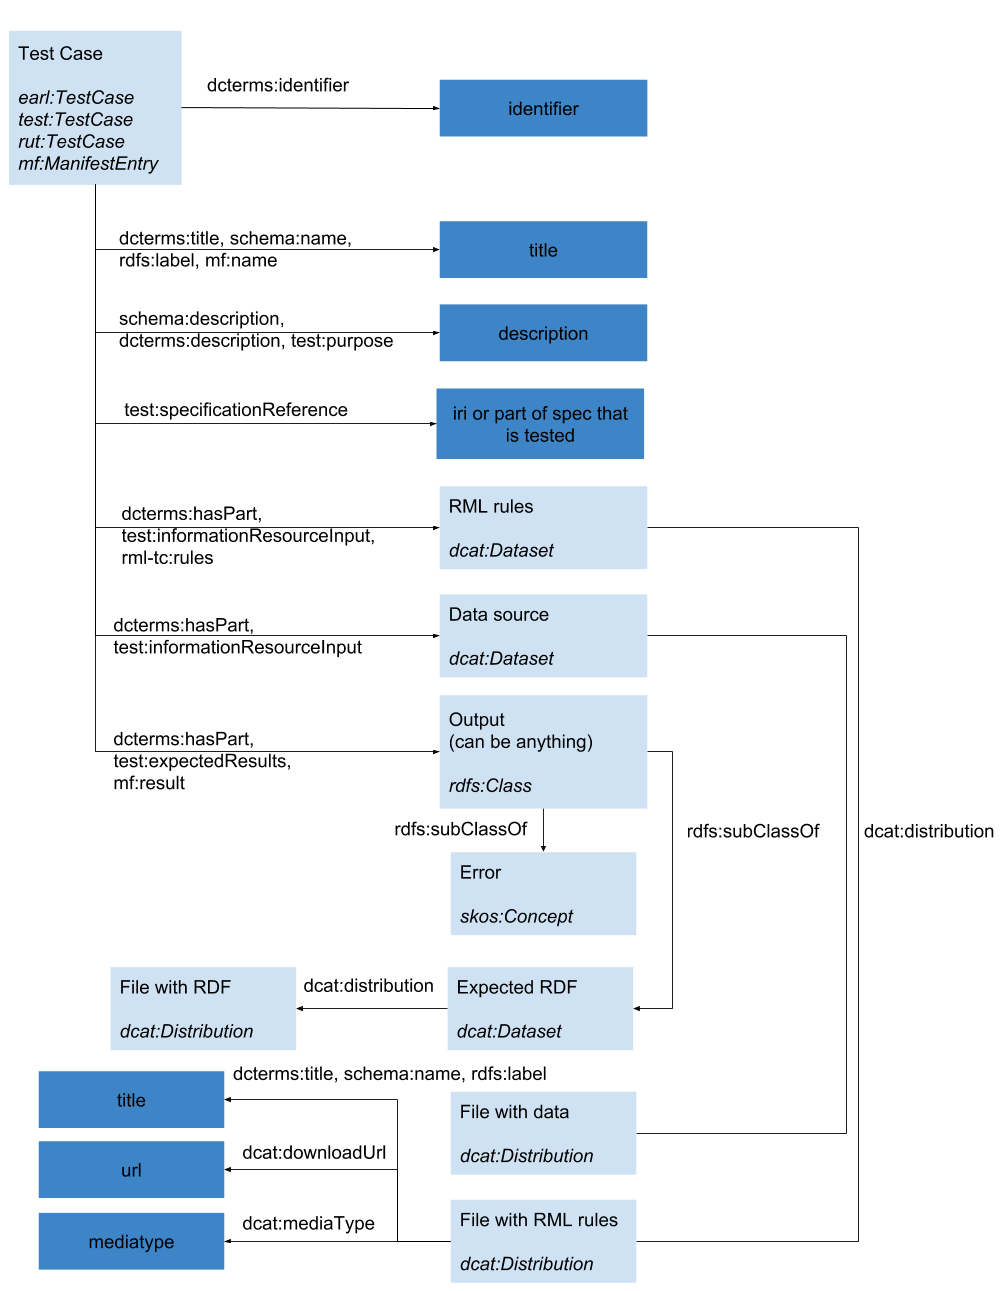
\includegraphics[width=0.9\textwidth]{figures/rml_test_case_model.png}
\caption{Data model of the RML test cases}
\label{fig:datamodel}
\end{figure}

In this section, we propose test cases to determine the conformance of RML processors to the RML specification. The proposed test cases are based on the R2RML test cases, but they take into account different heterogeneous data sources and the corresponding differences in RML. Our preliminary set of test cases includes (i)~adjusted R2RML test cases for relational databases (including MySQL\footnote{\url{https://www.mysql.com/}}, PostgreSQL\footnote{\url{https://www.postgresql.org/}}, and SQL Server\footnote{\url{https://www.microsoft.com/en-us/sql-server/}}) and (ii)~new test cases for files in the CSV, XML (with XPath as the reference formulation), and JSON format (with JSONPath as the reference formulation). The test cases are described at \url{http://rml.io/test-cases/} and the corresponding files are available at \url{https://github.com/rmlio/rml-test-cases}. In Section \ref{sec:datamodel}, we describe the data model that is used to represent the test cases. In Section \ref{sec:test-case-files}, we elaborate on the different files making up a test case. In Section \ref{sec:diff-r2rml-test-cases}, we discuss the differences between the R2RML and RML test cases.

\subsubsection{Data model}

We describe the test cases semantically to increase their reusability and sharability. To this end, we created a semantic data model\footnote{\url{http://rml.io/test-cases/\#datamodel}}, with as main entity the test case (see Figure \ref{fig:datamodel}). For each test case, the following details are described: unique identifier, title, description, relevant aspect of the RML specification, data sources (optional), expected knowledge graph or error, and RML rules.

To provide the corresponding semantic descriptions, the model uses mostly the Evaluation and Report Language (EARL) 1.0 Schema\footnote{\url{https://www.w3.org/TR/EARL10/}, with prefix \texttt{earl}}, the Test case manifest vocabulary\footnote{\url{http://www.w3.org/2001/sw/DataAccess/tests/test-manifest\#}, with prefix \texttt{mf}}, the Test Metadata vocabulary\footnote{\url{https://www.w3.org/2006/03/test-description\#}, with prefix \texttt{test}}, and the Data Catalog Vocabulary\footnote{\url{https://www.w3.org/TR/vocab-dcat/}, with prefix \texttt{dcat}}. A test case is annotated with the classes \verb|earl:TestCase|, \verb|test:TestCase|, and \verb|mf:ManifestEntry|. The identifier, title, description, and the specific aspect of the RML specification that is being tested are added as datatype properties. The files that are provided as input to the tools are linked to the test cases via \verb|test:informationResourceInput| and \verb|dcterms:hasPart|. The file with the RML rules is also linked via \verb|rml-tc:rules|\footnote{\url{http://rml.io/ns/test-cases}, with prefix \texttt{rml-tc}}. The objects of these properties are of the class \verb|dcat:Dataset|,which in turn link to a \verb|dcat:Distribution| that includes a link to a file. The expected output, whether that is a knowledge graph or an error, is linked via \verb|test:expectedResults|, \verb|mf:result|, and \verb|dcterms:hasPart|. In the case of a knowledge graph, the object of these properties is a \verb|dcat:Dataset|, linked to a \verb|dcat:Distribution|, to describe the file containing the graph. In the case of an error, we link to the expected error.

\subsubsection{Test case files}

Each test case consists of a set of files that contain the input data sources, the RML rules, and the expected RDF output. In practice, the files are organised as follows: all files for a single test case are contained in a single folder. There are three types of files for each test case:

\begin{itemize}
  \item 0 or more \textbf{data source files} for CSV (with extension .csv), XML (with extension .xml), and SON (with extension .json), or 
  1 file with SQL statements to create the necessary tables for relational databases (called \verb|resource.sql|);
  \item 1 \textbf{file with the RML rules} (in Turtle format, called \verb|mapping.ttl|); and
  \item 0 or 1 \textbf{file with the expected RDF} (in N-Quads format, called \verb|output.nq|).
\end{itemize}

Distinct test cases assess different behaviours of the processors. Certain test cases assess the behaviour of the tools when (i)~the required data sources are not available, and others when (ii)~an error occurs and no output is generated. In the former, no data sources files or SQL statements are provided. In the latter, no file with the expected RDF is provided. The test cases are independent of how the processors materialize the knowledge graph: a data dump, as done by the RMLMapper, or on the fly, as done by Ontario~\citep{endris2019ontario}.

\subsubsection{Differences with R2RML test cases}
For most R2RML test cases, we created an RML variant for CSV, XML, JSON, MySQL, PostgreSQL, and SQL Server, leading to 6 RML test cases per R2RML test case. For R2RML test cases that focus on specific features of SQL queries, we only created 3 RML test cases, i.e., for MySQL, PostgreSQL, and SQL Server.

For test cases with CSV, XML, and JSON files as data sources, we created the corresponding files with the data based on the tables of the relational databases. For CSV, we used the table created by the SQL statements of the R2RML test case and stored it as a CSV file. For XML, the name of the table was used for the root of the XML document and every row of the table was used to create an XML element. Within this element, elements were created for each column and their values are the values of the corresponding columns in the table. For JSON, we followed a similar approach as XML. The file contains a JSON object at the root with the name of the table as the only attribute. This attribute has as value an array, where each element of the array corresponds with a row in the table. For each row, attributes were created for each column and their values are the values of the corresponding columns in the table.

\paragraph{Data errors.}
2 of the R2RML test cases expect a data error to happen, e.g., when the subject IRI of an entity cannot be generated. In this case, an error is thrown and no knowledge graph is generated. With RML for entities where no subject IRI can be generated there is also no output generated, but, in contrast to R2RML, for the other entities the corresponding output is still generated. Therefore, for the corresponding RML test cases the processors can still throw an error, but the generation of the knowledge graph must not be halted.

\paragraph{Inverse expressions.}
3 of the R2RML test cases are designed to test the use of inverse expressions\footnote{\url{https://www.w3.org/TR/r2rml/\#inverse}}. However, inverse expressions are only used to optimize the knowledge graph generation and no differences are observed in the generated knowledge graph. Thus, whether inverse expressions are used by a processor or not cannot be verified by such test cases. Thus, we do not include them for RML.

\paragraph{SQL-specific features.}
18 of the R2RML test cases focus on specific features of SQL queries, e.g., a duplicate column name in a SELECT query. As there are no corresponding RML test cases for CSV files, XML files with XPath, and JSON files with JSONPath, we only provide 54 corresponding test cases for MySQL, PostgreSQL, and SQL Server.

\paragraph{Null values.}
1 of the R2RML test cases tests null values in the rows. However, a corresponding RML test case cannot be provided for the CSV and XML format, because both formats do not support null values.

\paragraph{Spaces in columns.}
1 of the R2RML test cases is designed to test the behaviour when dealing with spaces in the columns of the SQL tables. However, a corresponding RML test case cannot be provided for the XML format, because it does not allow spaces in names.
\\
\\
In total, we have 297 test cases: 39 for CSV, 38 for XML, 41 for JSON, and 180 for relational databases. Of these 297, 255 test cases expect an knowledge graph to be generated, while 36 expect an error that halts the generation.

\subsection{Conformance of RML Parsers}

In this section, we describe the executing of the test cases and their results for two RML processors: the RMLMapper and CARML. 
We detail on
(i) the method for running the test cases and obtaining the results, which are annotated semantically, and 
(ii) the implementation report similar as proposed for R2RML\footnote{\url{https://www.w3.org/TR/rdb2rdf-implementations/}}.  After this, we present the results of the RMLMapper and CARML. 

\subsubsection{Method}
We define a method to run the RML test cases over RML processors and generate the corresponding results. The main goal is to facilitate the testing process and provide a general solution for running the test cases over other RML processors that can be developed in the future. The method consists of two main steps: (i) assessing if a processor passes every test case and (ii) annotating the obtained results as RDF using the EARL Schema through a set of YARRRML rules~\citep{Heyvaert2018Declarative}.

We implemented a Java-based tool for checking the conformance of the test cases over different RML processors. At this moment, it is able to evaluate the test cases for JSON, CSV and XML formats. We relied on the test framework of each processor to execute the RDB test cases. If a new processor wants to be added to test its conformance, the framework only needs to have access to the corresponding output of each test-case. Then it checks, using the same method for all processors, if the output is the same as the correct one, if an error that is expected has really thrown, etc. The code is available online\footnote{\url{https://github.com/RMLio/rml-implementation-report}} together with a Web page showing the results of all tested tools\footnote{\url{http://rml.io/implementation-report}}. It generates as output two CSV files with the results and the metadata needed to generate the corresponding RDF.

%For obtaining the RDF from the results 
The results are semantically annotated, as the test cases, using the EARL Schema. Each test case evaluated by a tool is annotated as an \texttt{earl:Assertion} with the properties: \texttt{earl:subject} with the URI of the tool, \texttt{earl:assertedBy} with the identifier of who performed the evaluation, \texttt{earl:test} with the URI of the test and \texttt{earl:result} with the result of the test-case. 

Three types of results are possible: ``passed'', ``failed'', and ``inapplicable''. \textbf{Passed} (\texttt{earl:passed}) is used either when the actual output matches the expected output when no error is expected, or when the tool throws an error when an error is expected. \textbf{Failed} (\texttt{earl:failed}) is used either when the actual output does not match the expected output if no error is expected, the processor returns an error trying to execute a test or the tool does not throw error if an error is expected. \textbf{Inapplicable} (\texttt{earl:inapplicable}) is used when the tool clearly states that specific features used in a test case are not supported. 
%Together with this value, 
The results also provide its type (\texttt{earl:TestResult}) and its mode (\texttt{earl:automatic} for all these cases). 
We created a set of YARRRML rules to generate these annotations following the EARL Schema that, using the outputs of the test cases.
%generate the corresponding RDF.

\subsubsection{Results}
We perform the test-cases over two processors: RMLMapper and CARML. In Table \ref{tab:rmlmapper} we show the results for the RMLMapper processor. It passes all CSV, JSON and XML test cases, but fails in the same 5 test cases for the RDBs. The failures are related to the automatic datatyping of literal for RDBs specified by R2RML\footnote{\url{https://www.w3.org/TR/r2rml/\#dfn-natural-rdf-literal}}. RMLMapper expects to pass the failed test-cases in next versions of the processor. The effort prediction to pass these test-cases is not very much since the failures depend on the general processor, not on the used RDBMS. Once they have been solved for one RDBMS they will automatically pass over the rest.

In Table \ref{tab:carml} we show the results for the CARML processor. It partially passes the CSV, JSON and XML test cases, but it does not provide support for any of the RDBs test cases. The failures are related to the unsupported for multiple Subject Maps, multiple Predicate Maps, and Named Graphs. The developers of the tool declare that CARML will support these features in next versions of the processor. However, at the moment of writing, we do not have any information about if CARML will provide support for RDBs.

Finally, we can declare that testing a RML processor with the defined cases and analysing the obtained results offers a general view of the current status of it. These results also give useful information to the tool developers on knowing where they should put their effort to improve the conformance of the processor.

\begin{table}[]
\centering 
\caption[RML test-cases results for RMLMapper]{Results of the RMLMapper}
\label{tab:rmlmapper}
\renewcommand{\arraystretch}{1.5}
\begin{tabular}{c|c|c|c|c|c|c|c}

RMLMapper                 & \textbf{CSV} & \textbf{XML} & \textbf{JSON} & \textbf{MySQL} & \textbf{PostgreSQL} & \textbf{SQL Server} & \textbf{Total} \\ \hline
\textbf{passed}       & 39           & 41           & 38            & 55              & 55               & 55                   & 283             \\ \hline
\textbf{failed}       & 0           & 0           & 0            & 5              & 5                   & 5                   & 15             \\ \hline
\textbf{inapplicable} & 0            & 0             & 0             & 0             & 0                  & 0                  & 0            \\ 
\end{tabular}
\end{table}


\begin{table}[]
\centering
\caption{RML test-cases results for CARML}
\label{tab:carml}
\renewcommand{\arraystretch}{1.5}
\begin{tabular}{c|c|c|c|c|c|c|c}

CARML                 & \textbf{CSV} & \textbf{XML} & \textbf{JSON} & \textbf{MySQL} & \textbf{PostgreSQL} & \textbf{SQL Server} & \textbf{Total} \\ \hline
\textbf{passed}       & 29           & 28           & 28            & 0              & 0                   & 0                   & 85             \\ \hline
\textbf{failed}       & 10           & 10           & 13            & 0              & 0                   & 0                   & 33             \\ \hline
\textbf{inapplicable} & 0            & 0             & 0             & 60             & 60                  & 60                  & 180            \\ 
\end{tabular}
\end{table}

\section{Parameters that Affect the Construction of a Knowledge Graph}
\label{chapter5:sec-param}
In this section, we study the process of knowledge graph construction and analyze various variables and configurations that can impact on the performance of materialization techniques. The relevant parameters studied in this work include selectivity of the joins between mapping rules, types of relations, and percentage of duplicates. We also present diverse examples that evidence the heterogeneous behavior that each engine may exhibit whenever small changes are conducted to the variables and the configurations of a testbed.  

We devise a set of parameters involved in a knowledge graph construction process and we empirically show how they can impact on the behavior of two existing engines: RMLMapper\footnote{\url{https://github.com/RMLio/rmlmapper-java}} and SDM-RDFizer\footnote{\url{https://github.com/SDM-TIB/SDM-RDFizer}}; these engines are mostly fully compliant with the RML specification according to our results in the Section \ref{chapter5:sec-rml}. We develop a synthetic data generator for the generation of (semi)-structured data and RML mapping rules, that consider the identified set of parameters. The results of our empirical study provide evidence of the importance of the proposed set of variables and configurations during the evaluation of these tools. The testbeds used to conduct this evaluation are available
online\footnote{\url{https://github.com/SDM-TIB/KGC-Param-Eval}}.

Our main contribution includes the definition of various dimensions and set of variables to be considered during the creation of testbeds or to be measured while the evaluation of knowledge graph construction tools. Another contribution represents the empirical evaluation of the effects that the variables and configurations have on the tasks of knowledge graph construction. Furthermore, the results of the experimental study contribute to the understanding of the pros and cons of the studied engines, and the directions that need to be followed in order to devise tools able to scale up to real-world scenarios.  

\subsection{Motivation Example}

We motivate our work by analyzing different scenarios where the performance of RMLMapper and SDM-RDFizer may be affected by changing the configuration of the testbeds utilized for empirically evaluating these engines. We aim at remarking the importance of taking into account different parameters during the definition of a testbed. We first describe a scenario where na\"ive parameters (size and format) leads to wrong decisions during the comparing of SDM-RDFizer and RMLMapper. The testbeds include a data source with one thousand rows, different number of predicate-object (POM) in RML triple maps, and diverse configurations of selectivity of triple map joins.

%\begin{figure}[t!]
%	\centering
%	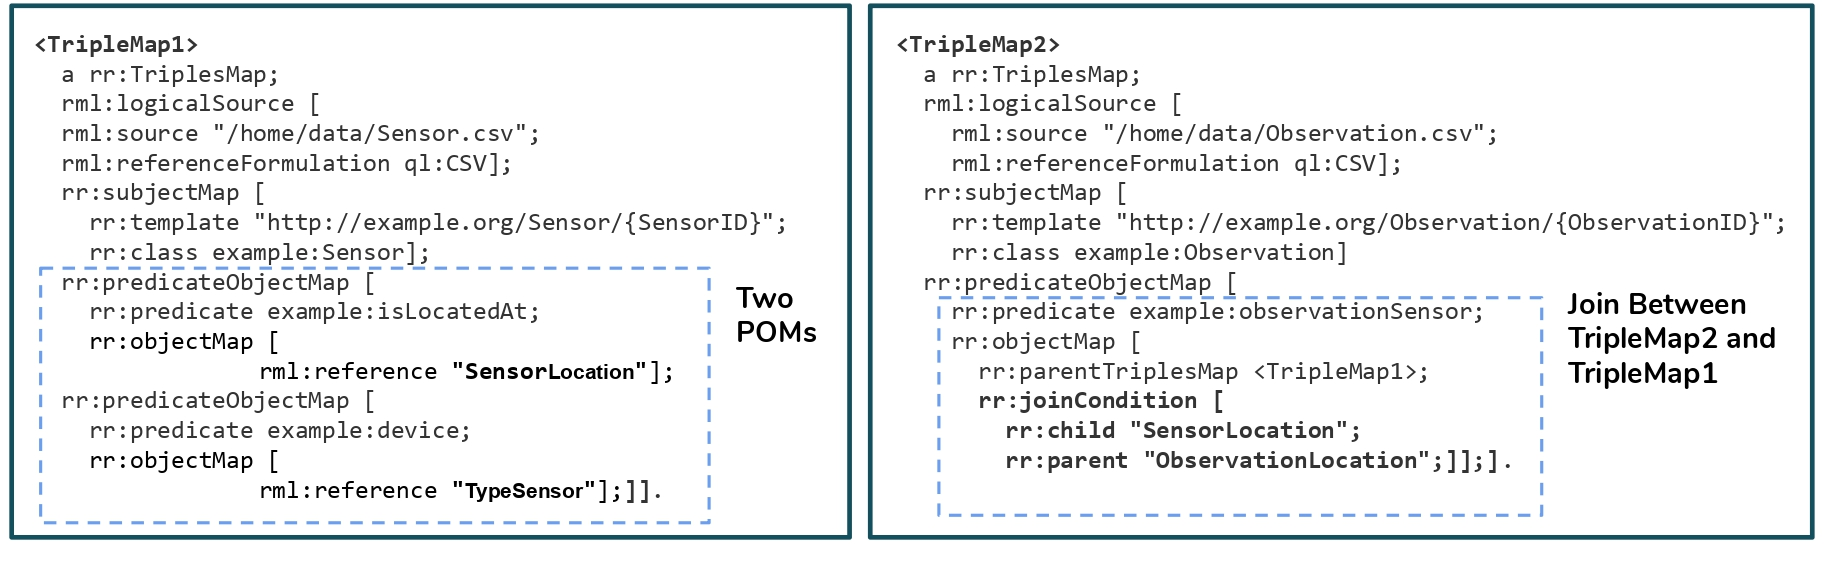
\includegraphics[width=\columnwidth]{figures/TripleMap.jpg}
%	\caption[RML Mapping example]{{\bf Motivating Example.} RML triple maps to transform two CSV files into RDF. TripleMap1 is composed of two predicate-object, i.e., Two POM. TripleMap2 has a join to TripleMap1; Observation.csv (outer relation) is joined to  Sensor.csv (inner relation) and the result, SensorID, is used as an object value.}
%	\label{fig:mappingRule}
%\end{figure}

%RML expresses mappings to transform sources represented in (semi)-structured format, e.g. CSV or XML, into RDF. Each mapping rule in RML, named RML triple map, is represented in RDF and consists of the following parts \citep{dimou2014rml}:
%\begin{itemize}
%    \item A \emph{Logical Source} that refers to a data source from where data is collected.
%    \item A \emph{Subject Map} that defines the subject of the generated RDF triples. 
%    \item \emph{Predicate-Object Maps} (POM) that expresses the predicate and the object the RDF triple to be generated; a triple map can comprise several POMs.
%\item
%A \emph{Referencing Object Map}, that indicates the reference or join condition to another triple map; the subject URL is the referenced triple map corresponds to the result of the evaluation of the join. 
%\end{itemize}
%\autoref{fig:mappingRule} illustrates two RML triple maps. \texttt{TripleMap1} is composed of two predicate-object maps, i.e. it is a Two POM mapping rule. \texttt{TripleMap2} has a referencing object map that joins the records of file Observation.csv with the records of the file Sensor.csv on the attributes \texttt{SensorLocation} and \texttt{ObservationLocation}. The result of executing the join between the two RML triple maps is the identifier of the sensor that collected the observation; this value is used as the object value of the predicate \texttt{observationSensor}.
%\subsubsection{Impact of Number of Predicates and Objects in Mapping Rules}
In this example, we execute a testbed where three different configurations of an RML mapping rule: Two-POM, Five-POM, and Ten-POM, i.e. they correspond to three mapping rules with two, five, and ten Predicate-Object Maps, respectively. 
Both engines exhibit a similar behavior while the number of predicate-object maps varies from two to five POMs, as shown in Table~\ref{tab:trivial}. However, when more complex mapping rules with more POMs are considered, the behavior of the SDM-RDFizer and RMLMapper is not impacted equally. Moreover, the results suggest that RMLMapper execution time increases with the number of POMs, while the SDM-RDFizer seems to be slightly affected. 
\begin{table}[ht!]
\centering
\caption[Impact of number of POMs on KGC engines]{\textbf{Impact of Number of Predicate-Object Maps.} Various predicate object maps (POM) specified in the mapping rules. The behavior of the two engines is similar when the mapping rules are simple (less than 5 POM) but it is different when more complex mappings are running (10 POM); time in seconds.
}
\label{tab:trivial}
\begin{tabular}{|l|c|c|}
\hline
\multicolumn{1}{|c|}{\multirow{2}{*}{\textbf{Engine}}} & \textbf{\begin{tabular}[c]{@{}c@{}}Execution \\ time (secs.)\end{tabular}} & \multicolumn{1}{l|}{\textbf{Number of results}} \\ \cline{2-3} 
\multicolumn{1}{|c|}{} & \multicolumn{2}{c|}{\textbf{Two POM}} \\ \hline
\multicolumn{1}{|c|}{\textbf{RMLMapper}} & 0.92  & 2,000 \\ \hline
\multicolumn{1}{|c|}{\textbf{SDM-RDFizer}} & 1.72 & 2,000 \\ \hline
\multicolumn{1}{|c|}{\textbf{}} & \multicolumn{2}{c|}{\textbf{Five POM}} \\ \hline
\textbf{RMLMapper} & 1.84 & 5,000 \\ \hline
\textbf{SDM-RDFizer} & 1.85 & 5,000 \\ \hline
 & \multicolumn{2}{c|}{\textbf{Ten POM}} \\ \hline
\textbf{RMLMapper} & 3.36 & 10,000 \\ \hline
\textbf{SDM-RDFizer} & 1.98 & 10,000 \\ \hline
\end{tabular}
\end{table}
%\subsubsection{Impact of Join Selectivity}
We now consider another parameter, the join selectivity, i.e. the cardinality of matching values from outer to the inner table (relation), in a referencing object map between two RML mapping rules. The join selectivity varies from 
\textbf{High Selectivity}, \textbf{Medium Selectivity}, and \textbf{Low Selectivity}, and Table~\ref{tab:joinSelectivity} reports on the results of RMLMapper and  SDM-RDFizer. First, it can be observed that the RMLMapper execution time increases by around $8$ seconds, while the SDM-RDFizer behavior is not equally affected by the selectivity of the join condition. As can be seen in Table~\ref{tab:joinSelectivity}, the SDM-RDFizer execution time (in seconds) increases from high to medium selectivity by $0.04$ (from $2.16$ to $2.20$), then decreases from medium to low selectivity by $0.01$ (from $2.20$ to $2.19$).
On the other hand, the RMLMapper execution time increases by $1.83$ (from $38.6$ to $40.43$), and $5.63$ (from $40.43$ to $46.06$) seconds from high to medium, and medium to low selectivity, respectively. As in the previous example, both engines are not equally affected by the complexity of the testbed. 

\begin{table}[ht!]
\centering
\caption[Impact of join selectivity on KGC engines]{\textbf{Impact of Join Selectivity.} Impact of the join selectivity variable over the engines with high, medium and low percentage of selectivity. While RMLMapper engine behavior increases in terms of execution time when the selectivity decreases, the SDM-RDFizer behavior is maintained, i.e. this variable affects to the first engine but it does not impact equality to the second one.}
\label{tab:joinSelectivity}
\begin{tabular}{|l|c|c|}
\hline
\multicolumn{1}{|c|}{\multirow{2}{*}{\textbf{Engine}}} & \textbf{\begin{tabular}[c]{@{}c@{}}Execution \\ time (secs.)\end{tabular}} & \multicolumn{1}{l|}{\textbf{Number of results}} \\ \cline{2-3} 
\multicolumn{1}{|c|}{} & \multicolumn{2}{c|}{\textbf{High Selectivity}} \\ \hline
\multicolumn{1}{|c|}{\textbf{RMLMapper}} & 38.6 & 2,100 \\ \hline
\multicolumn{1}{|c|}{\textbf{SDM-RDFizer}} & 2.16 & 2,100 \\ \hline
\multicolumn{1}{|c|}{\textbf{}} & \multicolumn{2}{c|}{\textbf{Medium Selectivity}} \\ \hline
\textbf{RMLMapper} & 40.43 & 23,000 \\ \hline
\textbf{SDM-RDFizer} & 2.20 & 23,000 \\ \hline
 & \multicolumn{2}{c|}{\textbf{Low Selectivity}} \\ \hline
\textbf{RMLMapper} & 46.06 & 30,000 \\ \hline
\textbf{SDM-RDFizer} & 2.19 & 30,000 \\ \hline
\end{tabular}
\end{table}

The uncorrelated behavior of studied engines shows clearly the need to considering diverse variables and configurations during the definition of testbeds, and thus, uncovering characteristics of these engines. In this work, we analyze the parameters that might affect a knowledge graph construction process and evaluate some of the most problematic ones (e.g. partitioning, relation type) to remark the importance of setting them during testbed design.  
 
\subsection{Relevant Parameters for Testbed Design}

{\small
\ctable[
	cap     = Variables and configurations that impact on KGC engines,
	caption =  \textbf{Variables and Configurations}. Set of variables and configurations that impact on the behavior of the tools for knowledge graph construction. Independent variables are divided into five groups and the impact on the observed variables is depicted., topcap,
	label   = {table:variables},
	maxwidth= 1.0\textwidth,
	pos = hb!,
]
%{c l c | c | c}
{X X c | c }
{
}{
\FL
% 
& &\multicolumn{2}{c}{\textbf{Observed Variables}}\NN
%\cmidrule(){3-5}
%   
\multicolumn{2}{c}{\multirow{2}{*}{ {\bf Independent Variables}}}  \\
%\multicolumn{2}{c}{ Observed Variables} &  Hidden Variables\\
\cmidrule(){3-4}
&	   & Execution Time & Completeness \ML
\multirow{10}{*}{\textbf{Mapping}}
        & mapping order				& \checkmark & \\
		& \# triplesMap 					& \checkmark & \checkmark  \\
		& \# predicateObjectMaps				& \checkmark & \checkmark \\ 
		& \# predicates				& \checkmark &\checkmark \\ 
		& \# objects				& \checkmark & \checkmark\\ 
		& \# joins				& \checkmark & \checkmark \\ 
		& \# named graphs				& \checkmark & \checkmark \\ 
		& join selectivity				& \checkmark & \checkmark \\  
		& relation type				& \checkmark & \checkmark \\ 
		& object TermMap type 			& \checkmark &        \ML
\multirow{5}{*}{\textbf{Data}}
        &  dataset size & \checkmark &                     		 \\
		&  data frequency distribution			& \checkmark &     \\
		&  type of partitioning		&   \checkmark                   & \checkmark  \\
		% &  \# sources		&   \checkmark                   &   \\
		&  data format 		& \checkmark & \checkmark  \ML
\multirow{3}{*}{\textbf{Platform}}
		&  cache on/off 				&      \checkmark              &   \\
		&  RAM available 				&         \checkmark            &    \\
		&  \# processors				&         \checkmark            &    
		\ML		
\multirow{3}{*}{\textbf{Source}}
		& distribution data transfer 					& \checkmark & \checkmark  \\
		& initial delay 					& \checkmark &   \\
		& access limitation     		      & \checkmark & \checkmark  
		\ML	
		%&  Sponge parameter	&    		      & \checkmark & \checkmark 
%
\multirow{3}{*}{\textbf{Output}}
		&  Serialization 				&      \checkmark              & \checkmark   \\
		&  Duplicates 				&         \checkmark            & \checkmark   \\
		&  Generation type				&         \checkmark            & \checkmark  
		\ML	
}
}

In this section, we perform a study of the parameters that have impact on the knowledge graph construction engines. First, we identify the generic groups of parameters involved and the effect they produce in this process. Second, we provide a list of specific variables that influence the construction of knowledge graphs and determine the relationships among them. Finally, we describe each parameter in detail given the reasons why it might affect the performance of the engines. Together with these descriptions, we provide use cases over a set of parameters to illustrate the importance of involving them in a testbed definition.

As in every empirical study, we consider two groups of variables: independent and observed. The independent variables are those features that need to be specified in a benchmark to ensure that the performed evaluation is reproducible. These variables are grouped in five dimensions: mapping, data, platform, source, and output.
On the other hand, observed variables correspond to those characteristics that are measured during the evaluation of the testbed and that may be influenced by independent variables. The observed variables are as follows:
\begin{itemize}
    \item \textit{Execution time:} The variable is in turn comprised of: \textit{i) Time for the first triple} (elapsed time between the engine starts and the first triple), \textit{ii) total execution time} required to produce all the triples of the knowledge graph.
    \item \textit{Completeness:} Number of returned triples in relation to all the RDF triples that should be created according to the data and input mappings.
\end{itemize}
The relations among independent and observed variables are presented in Table \ref{table:variables}. These variables are described in detail in the next section. 


\subsubsection{Mapping Dimension}
This dimension involves the variables that characterise the mappings in terms of their structure and evaluation. Regarding the structure, there are various aspects to be considered: mapping order, the complexity of the mapping in terms of number of predicates, objects, and the join type and selectivity.

\noindent \textbf{Mapping Order.} Although the mappings are usually defined using an RDF serialisation, where the order is not relevant, the features of each \texttt{rr:tripleMap} (e.g. joins) can affect the execution plan generated by each tool, having, thus, a potential negative impact on the total execution time.


\begin{table}[ht!]
\centering
\caption[Impact of relation types on KGC engines]{\textbf{Impact of Relation types.} Various relation types in a join specified in the mapping rules. N corresponds to 15 values in the case of 1-N and N-1 relations, N and M has 10 values in the last case. RMLMapper execution time is not affected by 1-N and N-1 relation types while it is affected by  N-M relations. SDM-RDFizer performs better in N-1 than 1-N but the time increases in N-M.}
\label{tab:relationType}
\begin{tabular}{|l|c|c|}
\hline
\multicolumn{1}{|c|}{\multirow{2}{*}{\textbf{Engine}}} & \textbf{\begin{tabular}[c]{@{}c@{}}Execution \\ time (secs.)\end{tabular}} & \multicolumn{1}{l|}{\textbf{Number of results}} \\ \cline{2-3} 
\multicolumn{1}{|c|}{} & \multicolumn{2}{c|}{\textbf{1-1}} \\ \hline
\multicolumn{1}{|c|}{\textbf{RMLMapper}} & 42.86 & 25,000 \\ \hline
\multicolumn{1}{|c|}{\textbf{SDM-RDFizer}} & 2.19 & 25,000 \\ \hline
\multicolumn{1}{|c|}{\textbf{}} & \multicolumn{2}{c|}{\textbf{1-N}} \\ \hline
\textbf{RMLMapper} & 43.34 & 22,490 \\ \hline
\textbf{SDM-RDFizer} & 2.19 & 22,490 \\ \hline
\textbf{} & \multicolumn{2}{c|}{\textbf{N-1}} \\ \hline
\textbf{RMLMapper} & 43.26 & 22,490 \\ \hline
\textbf{SDM-RDFizer} & 2.15 & 22,490 \\ \hline
 & \multicolumn{2}{c|}{\textbf{N-M}} \\ \hline
\textbf{RMLMapper} & 78.64 & 25,200 \\ \hline
\textbf{SDM-RDFizer} & 2.33 & 25,200 \\ \hline
\end{tabular}

\end{table}

\noindent \textbf{Mapping complexity.} The number of properties defined in a rule mapping, e.g. number of predicates, objects, or named graphs may affect the observed variables because the number of triples to be generated, is related to what is specified in the mappings. Additionally, the \texttt{rr:termtype} of the \texttt{rr:objectMap} can affect the total execution time because the cost of generating a constant or a template is not the same. Finally, the join selectivity and types of relation have also impact on the performance of an engine. In Table \ref{tab:relationType}, we illustrate how the relation type affects the total execution time of the studied engines. In this case, the behavior of the RMLMapper only occurs when the relation type is N-M. However, the SDM-RDFizer behavior is impacted during the evaluation of 1-N and N-M joins. Additionally, during the join evaluation, there are many cases when duplicates are generated, then the engines have to eliminate them. Table \ref{tab:duplicates} reports on how the generation of the duplicates --during the join condition evaluation-- affects the total execution time. RMLMapper decreases its performance while the percentage of duplicates increases. However,  SDM-RDFizer implements optimised data structured that allow for efficiently eliminating duplicates, and seems not to be equally affected by the complexity of these configurations, e.g. number of duplicates. 

\begin{table}[!tb]
\centering
\caption[Impact of duplicates on KGC engines]{\textbf{Impact of duplicates generation during join evaluation.} Various configurations of duplicates generated during the evaluation of a join between two triple maps. While the complexity of the configuration increases (more percentage of duplicates), the RMLmapper decreases its performance. Surprisingly, the SDM-RDFizer seems not to be affected by the complexity of the testbeds, and improves its performance even when the complexity of testbeds increases.}
\label{tab:duplicates}
\begin{tabular}{|l|c|c|}
\hline
\multicolumn{1}{|c|}{\multirow{2}{*}{\textbf{Engine}}} & \textbf{\begin{tabular}[c]{@{}c@{}}Execution \\ time (secs.)\end{tabular}} & \multicolumn{1}{l|}{\textbf{Number of results}} \\ \cline{2-3} 
\multicolumn{1}{|c|}{} & \multicolumn{2}{c|}{\textbf{Low percentage of duplicates}} \\ \hline
\textbf{RMLMapper} & 37.94 & 20,027 \\ \hline
\textbf{SDM-RDFizer} & 2.01 & 20,027 \\ \hline
\multicolumn{1}{|c|}{\textbf{}} & \multicolumn{2}{c|}{\textbf{Medium percentage of duplicates}} \\ \hline
\textbf{RMLMapper} & 39.201 & 20,105 \\ \hline
\textbf{SDM-RDFizer} & 1.87 & 20,105 \\ \hline
\textbf{} & \multicolumn{2}{c|}{\textbf{High percentage of duplicates}} \\ \hline
\textbf{RMLMapper} & 40.81 & 20,263 \\ \hline
\textbf{SDM-RDFizer} & 1.89 & 20,263 \\ \hline
\end{tabular}
\end{table}

\subsubsection{Data Dimension}
We describe the independent variables related with the original data that are required for the generation of a knowledge graph. Each dataset can be defined in terms of \textbf{size} and \textbf{total number of sources}. The first characteristic impacts on the number of triples that will be generated, affecting, thus, the total execution time. Additionally, the total number of sources that have to be processed to generate a knowledge graph may also affect the total execution time.

\noindent \textbf{Partitioning} and \textbf{distribution} are important variables considered in the construction of a knowledge graph. Partitioning refers to the way that a dataset is fragmented, and distribution is the format (e.g. CSV, JSON) of each partition. A dataset can be presented in only one format or in multiples formats, and this variable affects not only the total execution time but also the completeness of the results. A dataset may be fragmented into disjointed partitions; the partition may be horizontal, vertical or a combination of both. Horizontal partitioning fragments the dataset, so that, they represent different instances of the same resource (equal \textit{TripleMaps} with different sources). Vertical partitioning produces fragments that contain at least one property of the same resources (\textit{TriplesMaps} with \textit{JoinCondition}). The horizontal partitioning may affect the completeness of a knowledge graph while the vertical partitioning has an influence on the execution time. Table \ref{tab:partitioning} compares the behavior of the RMLMapper and SDM-RDFizer with different configurations. The two engines increase their execution time when the horizontal partitioning is compared with and without including replication. However, RMLMapper decreases its execution time when the vertical partitions with and without replication are compared, while SDM-RDFizer execution time increases.  Thus, even SDM-RDFizer is tailored towards efficient duplicate elimination, data partitioning-- with and without replication -- seems to affect the SDM-RDFizer performance. \newline

% Please add the following required packages to your document preamble:
% \usepackage{multirow}
\begin{table}[!tb]
\centering
\caption[Impact of partitioning on KGC engines]{\textbf{Impact of Partitioning}: Various configurations of vertical and horizontal partitioning with and without duplicates. The two engines perform similar with the two cases of the horizontal partitioning but they have different behaviors in vertical partitioning.}
\label{tab:partitioning}
\begin{tabular}{|l|c|c|}
\hline
\multicolumn{1}{|c|}{\multirow{2}{*}{\textbf{Engine}}} & \textbf{\begin{tabular}[c]{@{}c@{}}Execution \\ time (secs.)\end{tabular}} & \textbf{Number of results} \\ \cline{2-3} 
\multicolumn{1}{|c|}{} & \multicolumn{2}{c|}{\textbf{Horizontal Partitioning without Replication}} \\ \hline
\textbf{RMLMapper} & 1,904.31 & 310,000 \\ \hline
\textbf{SDM-RDFizer} & 4.84 & 310,000 \\ \hline
\multicolumn{1}{|c|}{\textbf{}} & \multicolumn{2}{c|}{\textbf{Vertical Partitioning without Replication}} \\ \hline
\textbf{RMLMapper} & 2,067.77 & 310,000 \\ \hline
\textbf{SDM-RDFizer} & 4.73 & 310,000 \\ \hline
\textbf{} & \multicolumn{2}{c|}{\textbf{Horizontal Partitioning with Replication}} \\ \hline
\textbf{RMLMapper} & 2,276.98 & 310,000 \\ \hline
\textbf{SDM-RDFizer} & 5.86 & 310,000 \\ \hline
\textbf{} & \multicolumn{2}{c|}{\textbf{Vertical Partitioning with Replication}} \\ \hline
\textbf{RMLMapper} & 2,024.66 & 310,000 \\ \hline
\textbf{SDM-RDFizer} & 4.98 & 310,000 \\ \hline
\end{tabular}
\end{table}

\subsubsection{Platform Dimension}
The platform dimension comprises variables related with the hardware used to create a knowledge graph. We include a set of variables related with the system cache, the available RAM memory for running the tool, and the number of processors of the machine. The \textbf{cache} and the \textbf{available RAM memory} may affect the total time execution.  We recommend that other parameters, like the versions of operating system and processor, should be specified in the evaluation setup. To conclude, during testbed design, the platform and hardware specification requires attention and  needs to be defined in detail.

\subsubsection{Source Dimension}
In this dimension, we consider different variables related with the original sources defined in the mapping rules. The \textbf{distribution data transfer}, which corresponds to the transfer time of a file by a Web service--in case the data is not in a local machine-- will definitely influence the total execution time. Additionally, the \textbf{initial delay} of each engine to configure the corresponding wrappers for each data format and the \textbf{limit access} for example, a database, also strikes out the execution time and the completeness of the results.

\subsubsection{Output Dimension}
In this dimension, we consider the variables related with the output of the generation process. The \textbf{serialization} impacts on the total execution time; the effect will depend on the size of the output and the number of times the processor has to access the disk to store the output. \textbf{Generation type} represents how an engine constructs a knowledge graph. The generation can be continuous, e.g. the SDM-RDFizer stores each RDF triple in a file once it is generated. Contrary, the generation can be in-memory, e.g. RMLMapper stores the output when the knowledge graph is created completely. Finally, the engines usually can have a flag for removing \textbf{duplicates}; this operation has to be specified in the setup because it strikes out the completeness and also the total execution time. The efficiency of the engines components that eliminate duplicates, can be captured by observing the variables of this dimension.   

As can be observed in the results reported in this section, the behavior of the studied engines is not equally affected by the different independent variables. Thus, benchmarks need to include all these variables in order to provide a holistic overview of the performance of the studied engines, and ensure general and reproducible evaluations. 


\subsection{Evaluation of affected parameters in KGC}
The goal of our experiment is to assess the impact of the discussed variables and configurations during the evaluation of existing knowledge graph construction tools. We aim at answering the following research questions: \textbf{RQ1}:What is the effect of mixing different variables in one testbed?; \textbf{RQ2}: What is the impact of considering configurations of different complexity of the same variable in one testbed?; \textbf{RQ3}: Do the different variables and configurations influence in the behavior of existing knowledge graph construction tools? To answer these research questions, we set up the following experimental studies:

\noindent \textbf{Datasets.}
For this evaluation, we generated three different datasets with 1,000 (1K), 10,000 (10K), and 50,000 (50K) rows, and various number of columns based on the tested parameters; ~\autoref{tab:datasets} shows the properties of the datasets generated for \texttt{Relation Type}, \texttt{Join Duplicates}, and \texttt{Join Selectivity} evaluations. 
For the \textit{Dataset Size (N{\"a}ive)} parameter, we generated the same number of rows as in~\autoref{tab:datasets}, but with $30$ columns.
\begin{table}[!tb]
    \centering
    \caption[Testbeds for Analyzing the Impact over KGC engines]{\textbf{Datasets.} Properties of Datasets used in the Empirical Evaluations.}
    \label{tab:datasets}
    \begin{tabular}{|c|c|c|c|}
    \hline
     Dataset & \#rows & \#columns & \#tables \\ \hline
     1K & 1,000 & 2 & 2 \\ \hline 
     10K & 10,000 & 2 & 2 \\ \hline 
     50K & 50,000 & 2 & 2 \\ \hline 
     \end{tabular}
\end{table}
%
During the experiments, we only considered the CSV file format to represent the generated tables.

\begin{figure}[!tb]
    \centering
    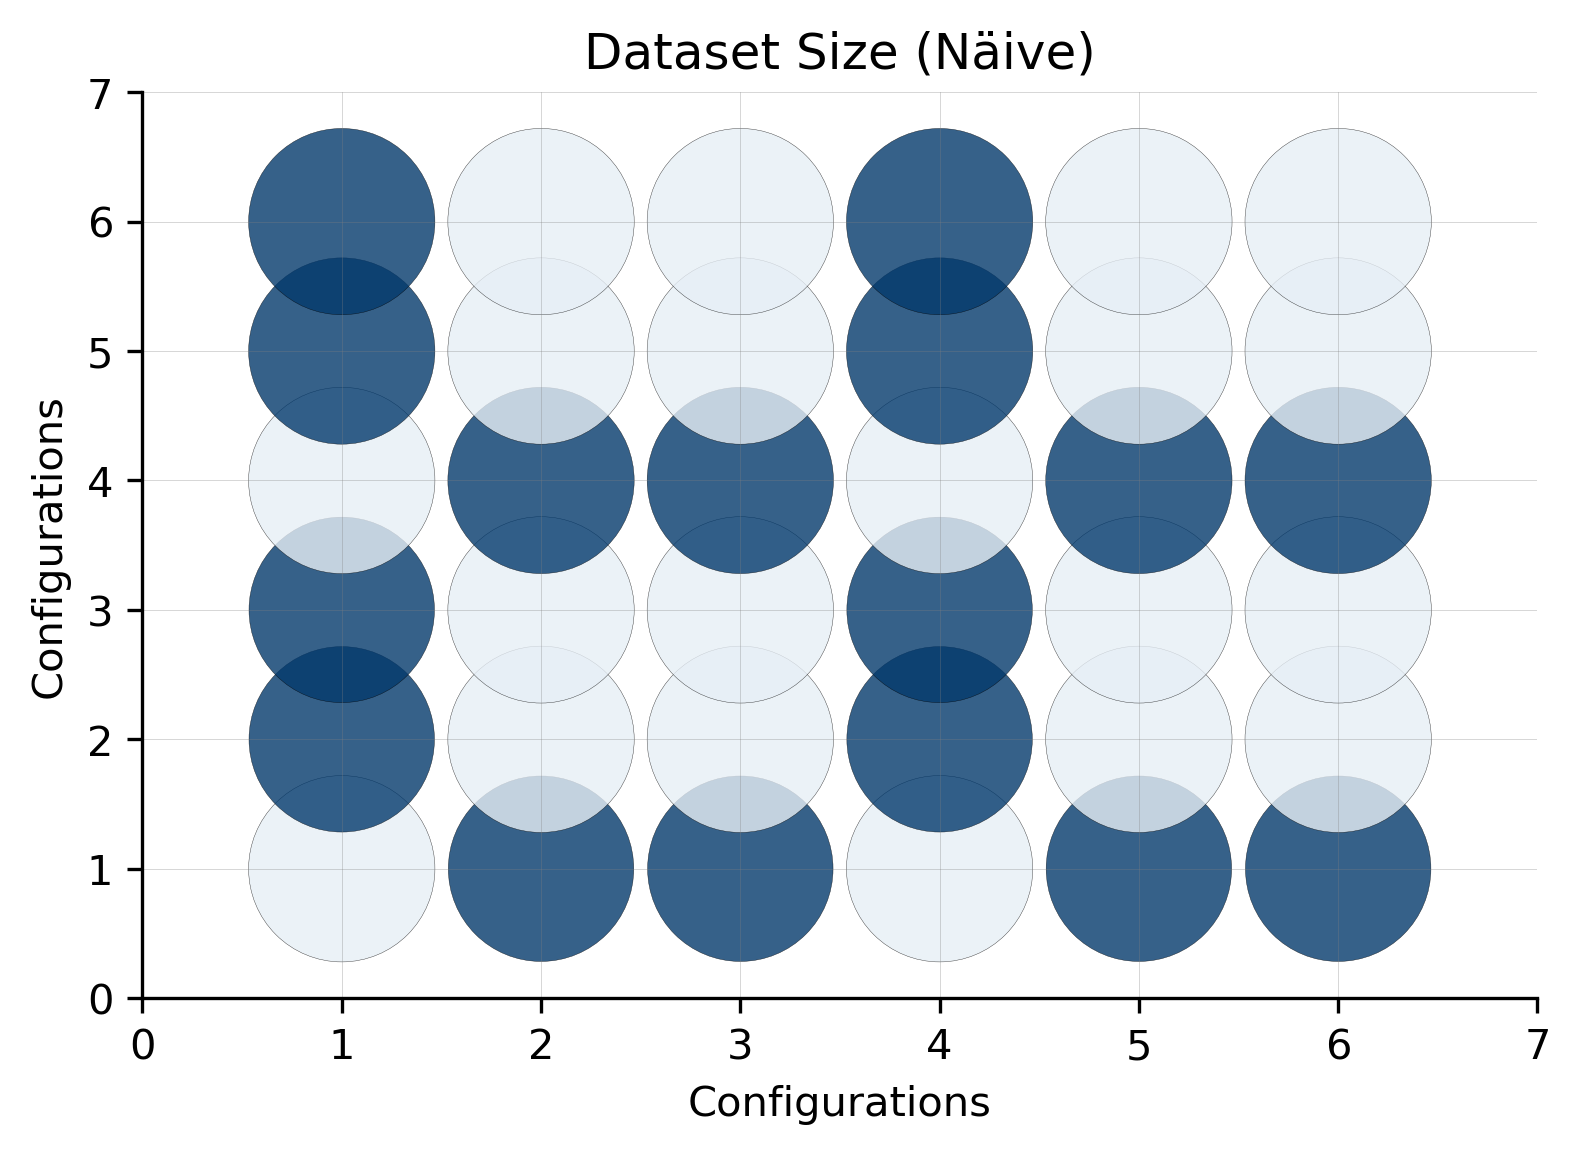
\includegraphics[width=0.8\columnwidth]{figures/naive_allk_bubble.png}
    \caption[Knowledge Graph Construction Tools on Different Dataset Sizes (Na{\"i}ve)]{\textbf{Comparison of Knowledge Graph Construction Tools on Different Dataset Sizes (Na{\"i}ve).} The first three configurations, i.e. 1, 2, and 3 in x-axis and y-axis, correspond to SDM-RDFizer on datasets 1K, 10K, and 50K, respectively. The last three configurations, i.e. 4, 5, and 6 on x-axis and y-axis, correspond to RMLMapper 1K, 10K, and 50K, respectively. Grey bubbles correspond to correlation value of $1.0$; blue bubbles show a positive correlation. The number of blue bubbles suggests that both systems exhibit similar behavior.}
    \label{fig:naive_bubble}
\end{figure}

\noindent \textbf{Configurations.}
We consider different configurations for the above-discussed variables in each dimension. 
%
\texttt{Dataset Size Configurations:} 1) SDM-RDFizer 1K; 2) SDM-RDFizer 10K; 3) SDM-RDFizer 50K; 4) RMLMapper 1K; 5) RML\-Mapper 10K; and 6) RMLMapper 50K. In each configuration of this parameter, we only use one data file.
%
\texttt{Relation Type configurations:} 1) SDM-RDFizer 1-N; 2) SDM-RDFizer N-1; 3) SDM-RDFizer N-M; 4) SDM-RDFizer Combinations (all relation types); 5) RMLMapper 1-N; 6) RMLMapper N-1; 7) RMLMapper N-M; and 8) RMLMapper Combinations (all relation types). For relation cardinality, we evaluated $N=\{1, 5, 10, 15\}$ and $M=\{1, 3, 5, 10\}$. In addition, we set the percentage of rows that involve in those relation types to $25\%$, i.e. $25\%$ of the overall rows from outer table have a matching join value to inner table, and $50\%$, respectively.
%
\texttt{Join Duplicate configurations:}  1) SDM-RDFizer Low, 2) SDM-RDFizer High, 3) RMLMapper Low, 4) RMLMapper High. \texttt{Low} Join Duplicates refer to datasets with low percentage of duplicates, i.e. from $5\%$ to $20\%$ of data generated could have duplicates due to the join conditions, similarly 
\texttt{High} Join Duplicates refer to higher percentage of duplicates, i.e. from $30\%$ to $50\%$ of data generated could be duplicated. 
%
\texttt{Join Selectivity Configurations:} 1) SDM-RDFizer High; 2) SDM-RDFizer Low; 3) RMLMapper High; and 4) RMLMapper Low. In this case, the join selectivity \texttt{High} represents how many time the join condition matches the values in the inner join file from 5\% to 20\% of the overall rows, while \texttt{Low} means that the join condition matches range from 60\% to 100\% of the overall number of rows. As previously shown, we hypothesise that these configurations allow us to uncover patterns in the behavior of these engines that could not be observed if only na{\"i}ve variables were studied. 

\noindent \textbf{Metrics}
We report on the following metrics or observed variables: 
\textit{Execution Time}: Elapsed time between execution of an engine and the delivery of the results.
\textit{Number of Results}: Number of triples generated by the KGC engine.

\noindent \textbf{Implementations.} 
The SDM-RDFizer and the testbeds are implemented in Python 3.6; the SDM-RDFizer is publicly available\footnote{\url{https://github.com/SDM-TIB/SDM-RDFizer}}. Furthermore, Jupiter Notebooks are available to generate the data and plot the results. Additionally, we have created a Docker image to run the testbeds and reproduce the experimental results\footnote{\url{https://github.com/SDM-TIB/KGC-Param-Eval}}. The experiments were run in an Intel(R) Xeon(R) equipped with a CPU E5-2603 v3 @ 1.60GHz 20 cores, 100G memory with Ubuntu 16.04LTS.


\begin{figure}[!tb]
    \centering
    \subfloat[Dataset 1K]{
      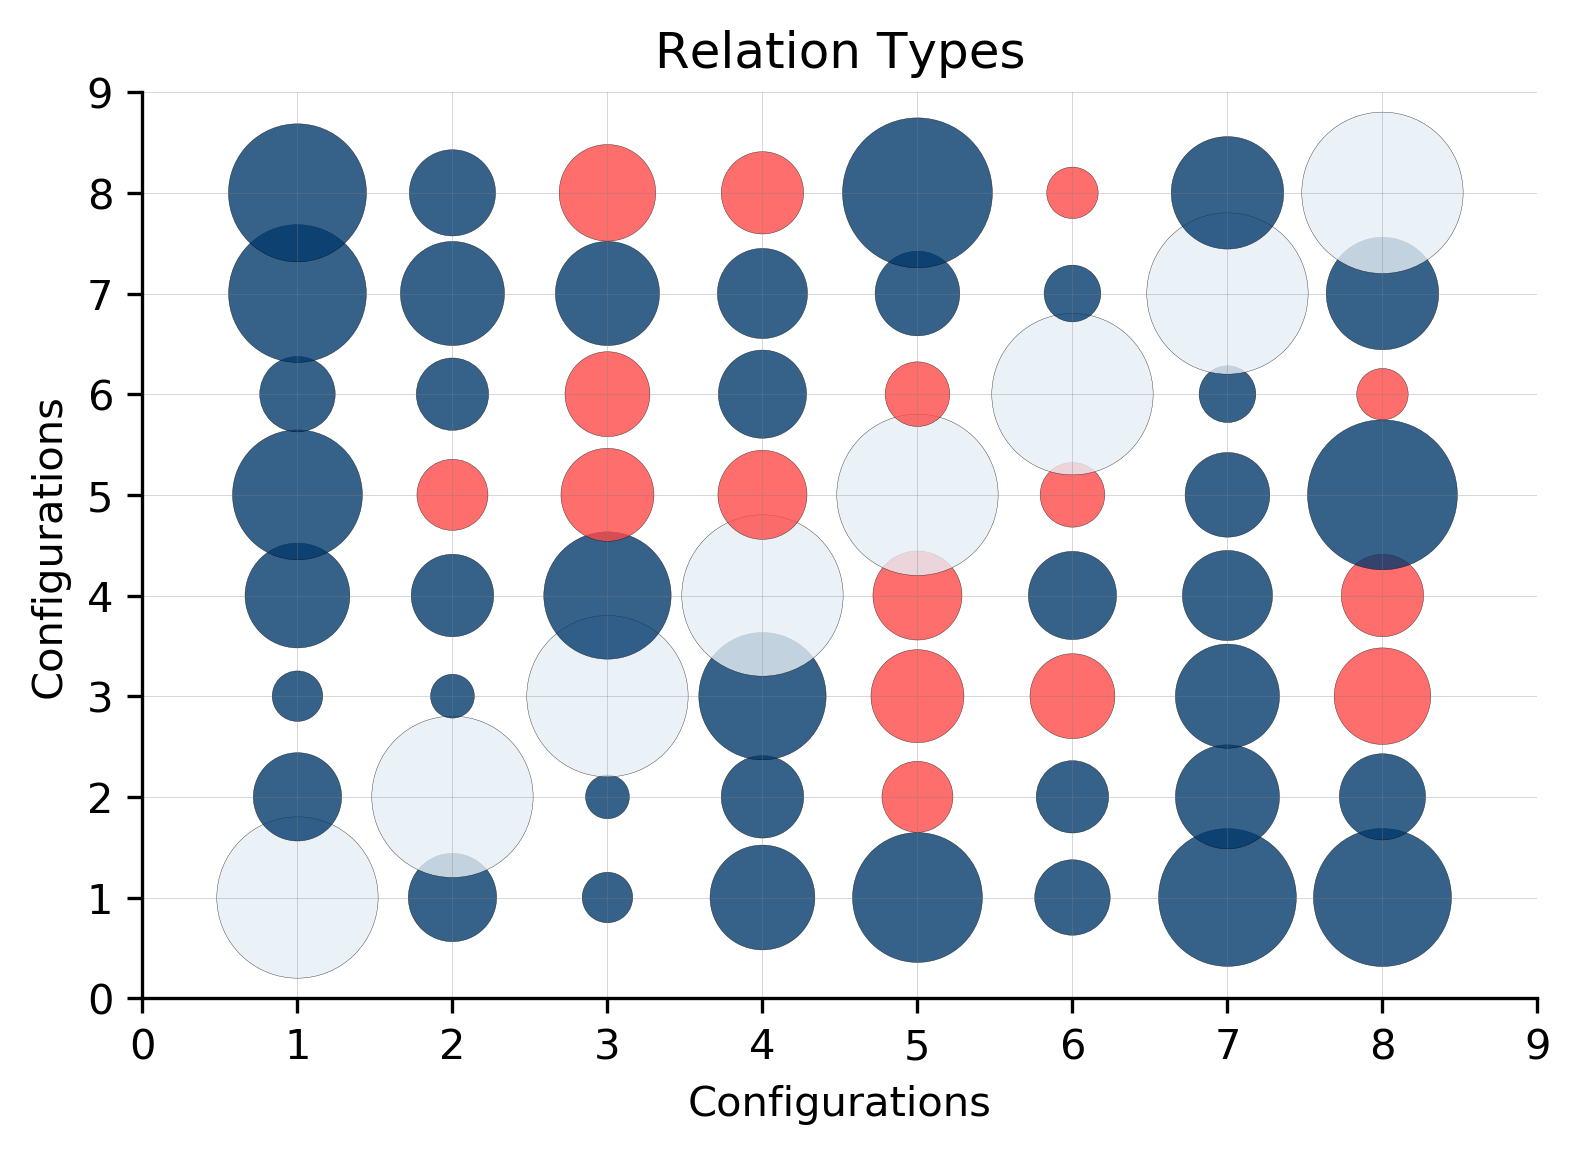
\includegraphics[width=0.48\columnwidth]{figures/relation_type_01k_bubble.png}
      \label{fig:rt_1k}
    }
    \subfloat[Dataset 10K]{
      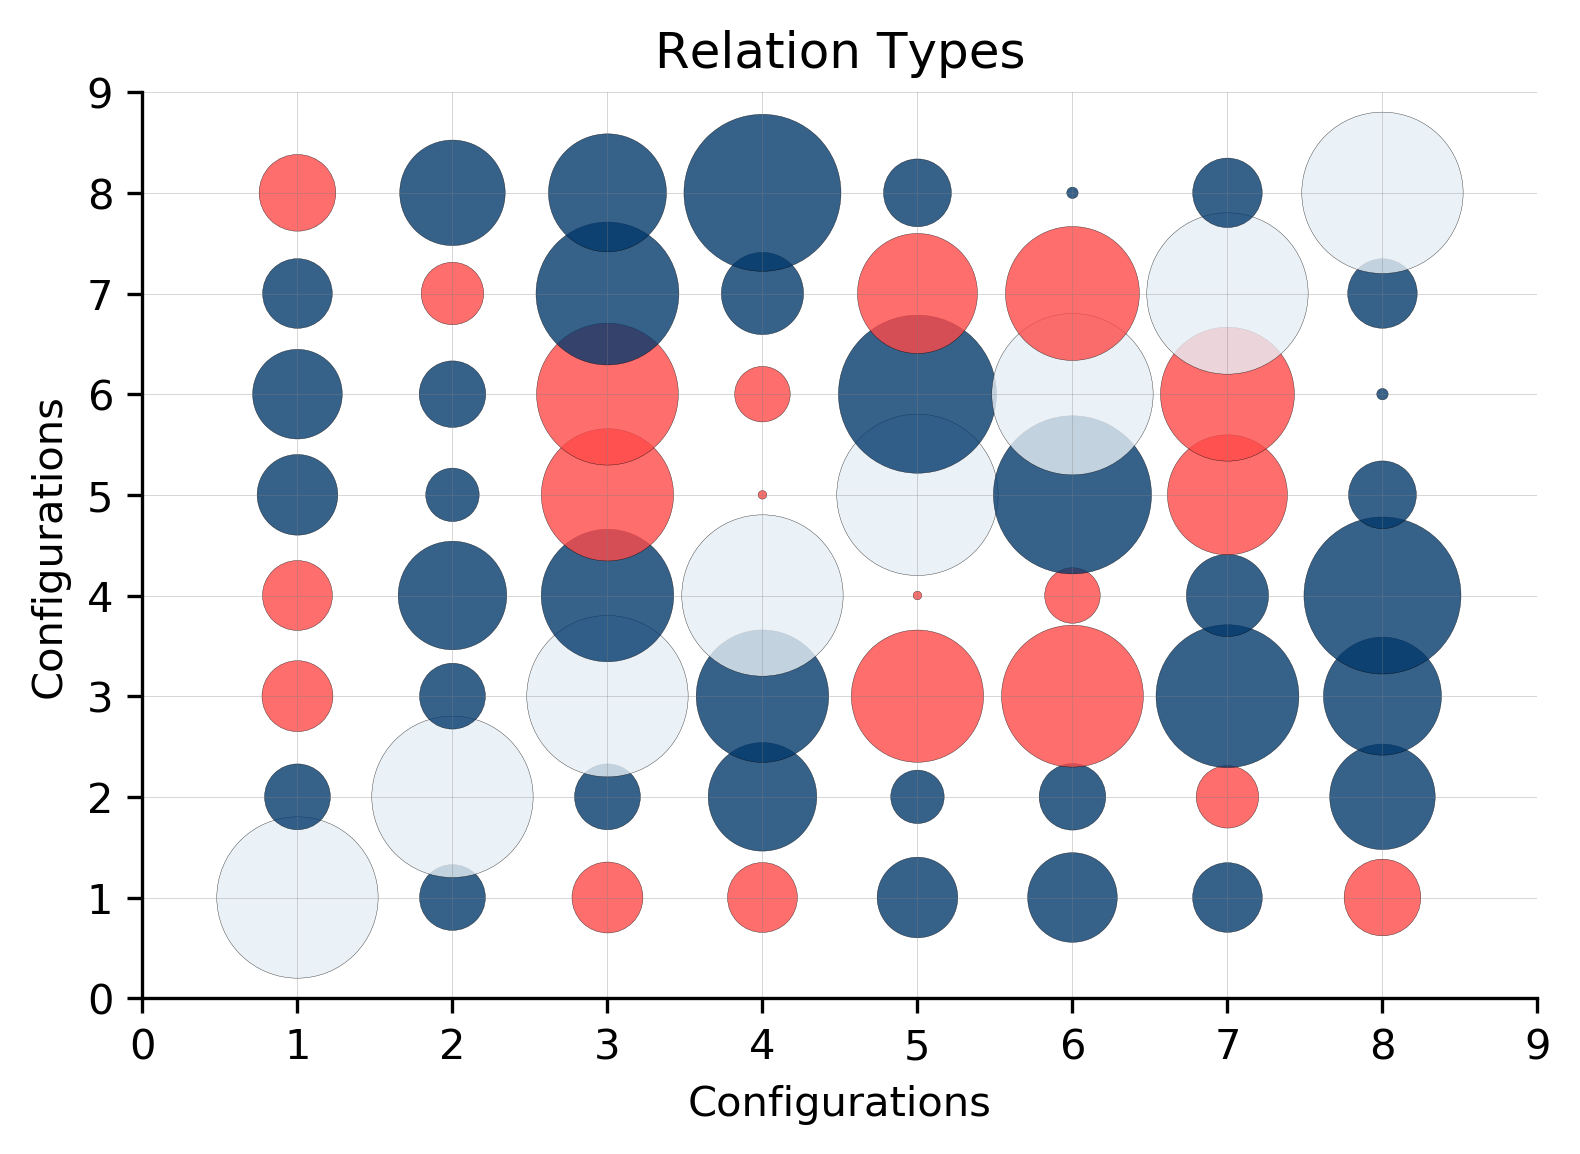
\includegraphics[width=0.48\columnwidth]{figures/relation_type_10k_bubble.png}
      \label{fig:rt_10k}
    }
    \qquad
    \subfloat[Dataset 50K]{
      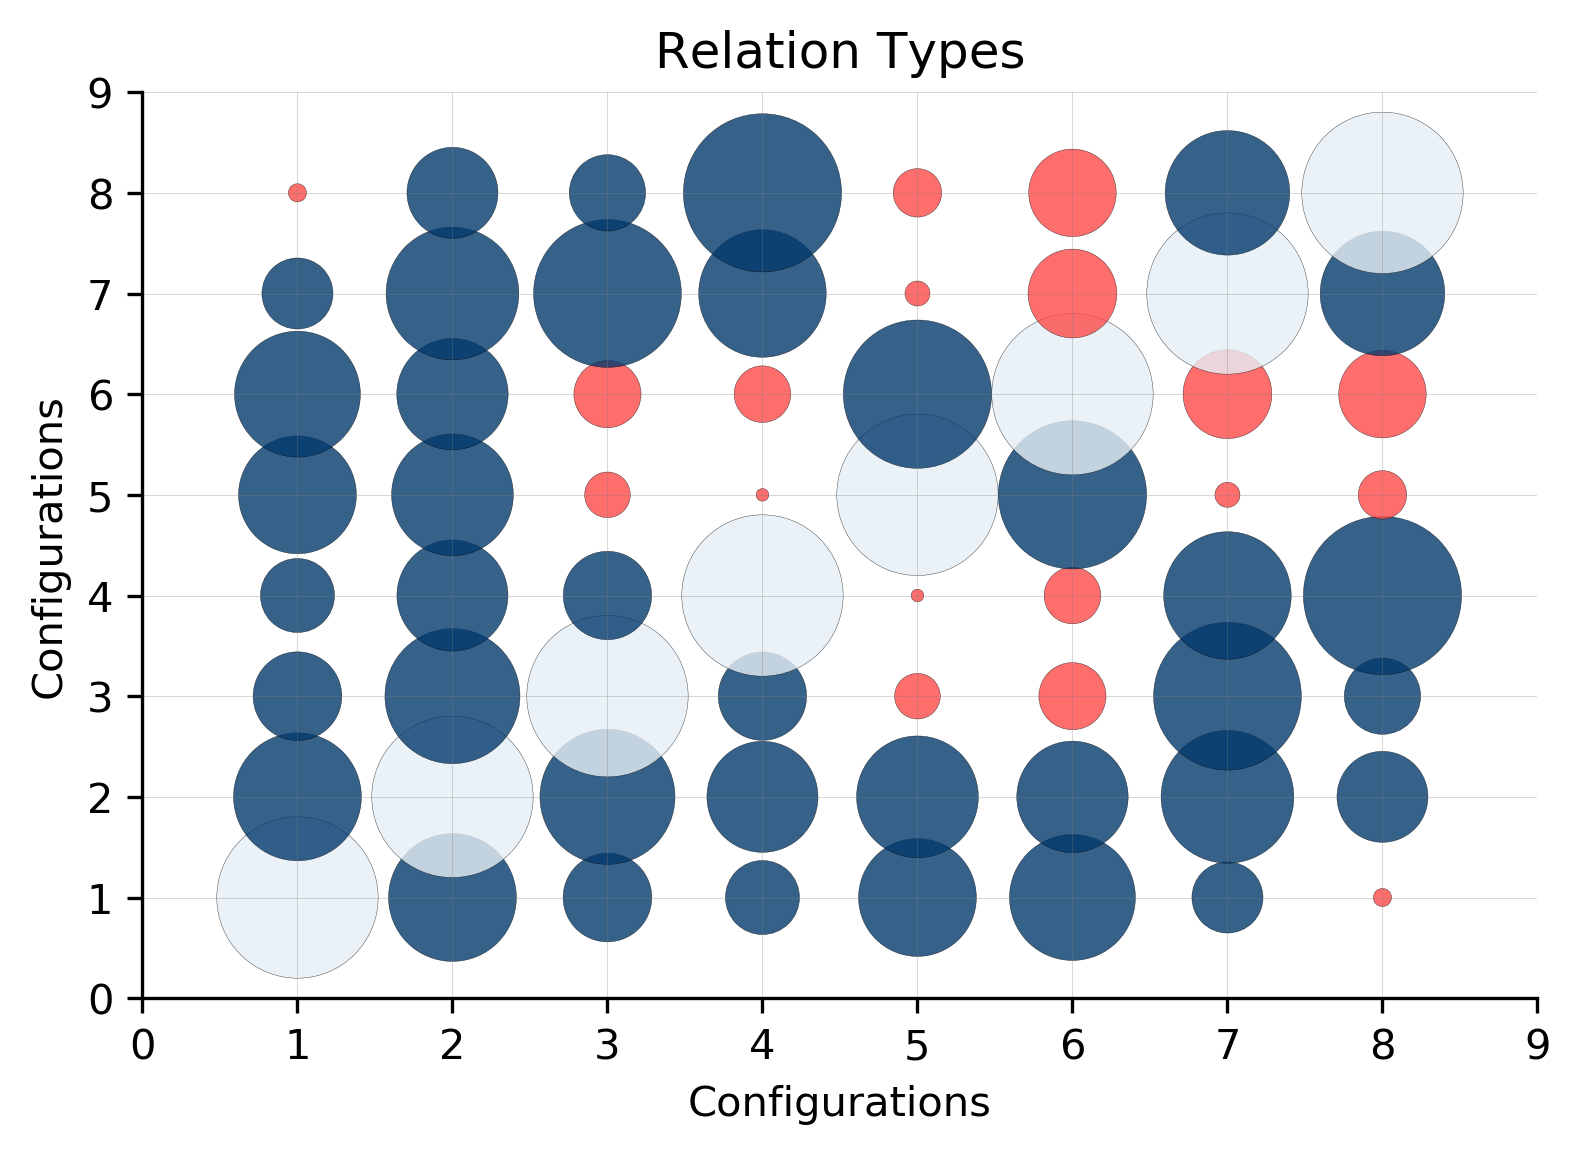
\includegraphics[width=0.48\columnwidth]{figures/relation_type_50k_bubble.png}
      \label{fig:rt_50k}
    }
    \subfloat[Combination of 1K, 10K, and 50K]{
      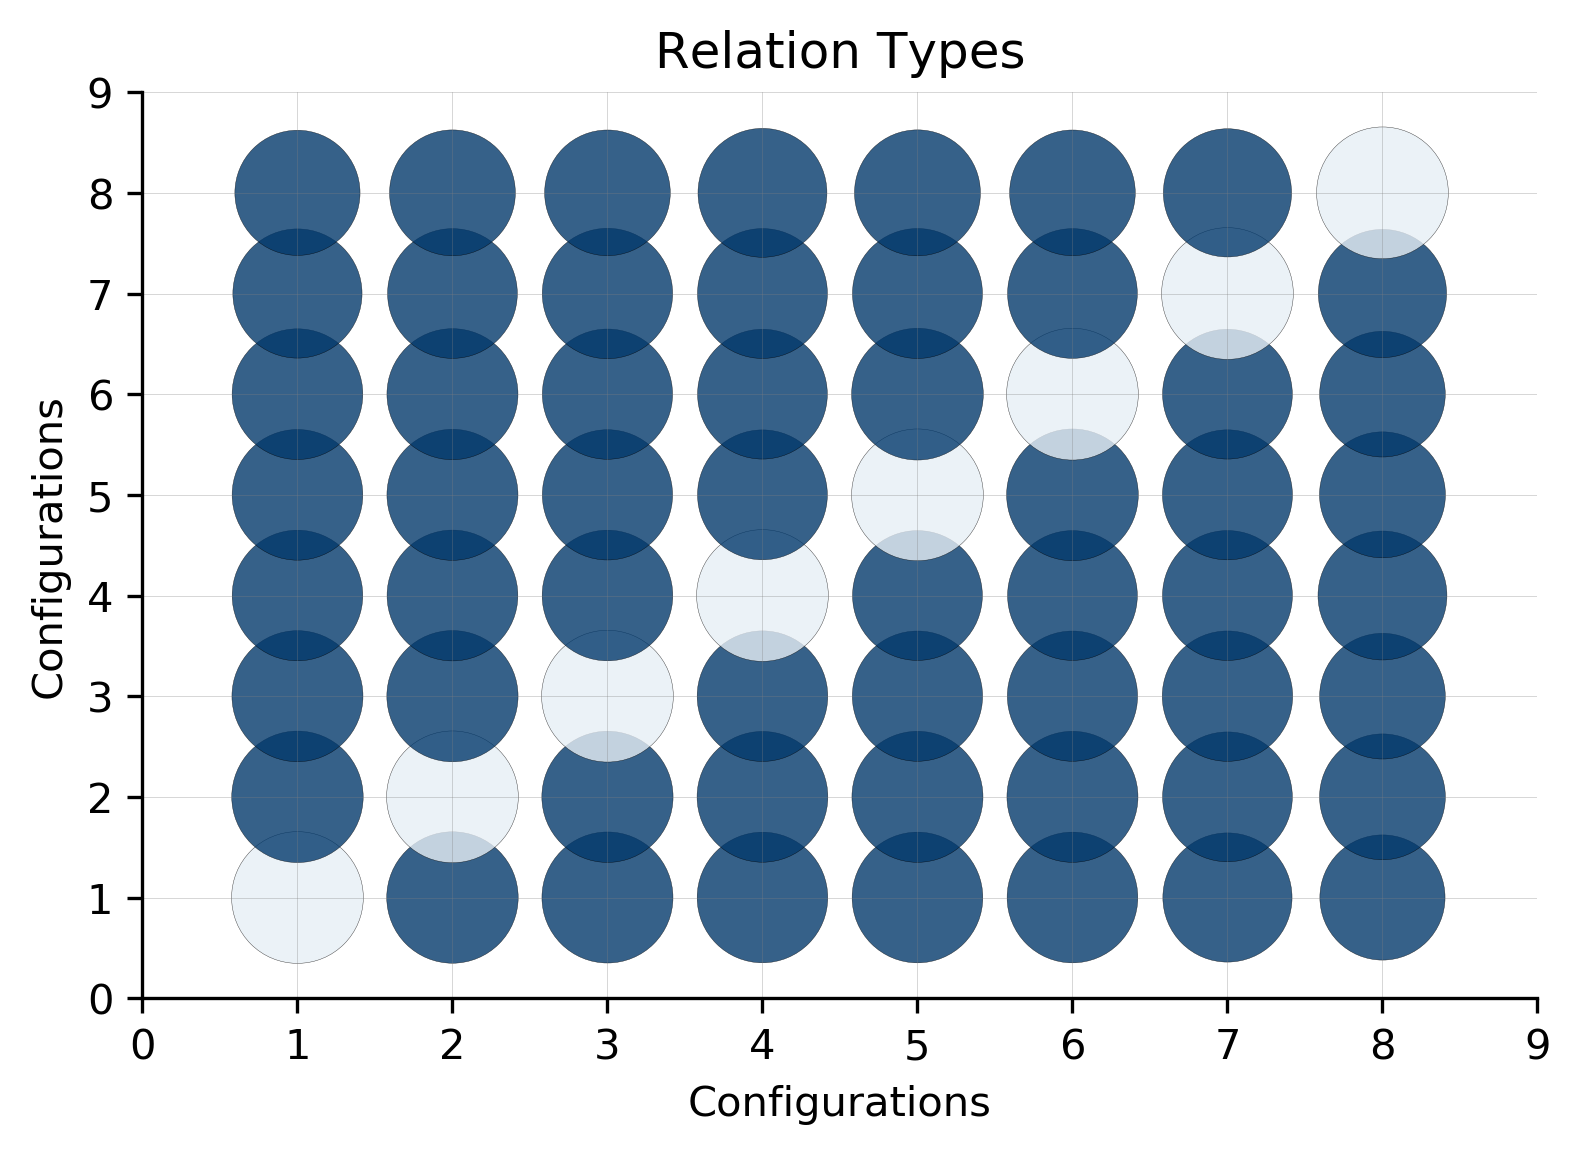
\includegraphics[width=0.48\columnwidth]{figures/relation_type_allk_bubble.png}
      \label{fig:rt_all}
    }
    \caption[Knowledge Graph Construction Tools on Different Types of Relations]{\textbf{Comparison of Knowledge Graph Construction Tools on Different Types of Relations.} The first four (4) configurations, i.e. 1-4 in both x-axis and y-axis, represent results of SDM-RDFizer on \textit{1-N}, \textit{N-1}, \textit{N-M}, and combination of all relations types, respectively. The later configurations, 5-8 both in x-axis and y-axis, shows results of RMLMapper on \textit{1-N}, \textit{N-1}, \textit{N-M}, and combination of all relations types, respectively. Grey bubbles correspond to correlation value of $1.0$; blue bubbles show a positive correlation while red bubbles show a negative correlation. The plots reveal that both type of relations and size of the dataset need to be taken into account to uncover patterns in the behavior of the engines. 
    }
    \label{fig:relation_type_bubble}
\end{figure}


\noindent \textbf{Testbeds.}
Results of each configurations are ordered from lower to higher complexity and compared using the Pearson's correlation. 
A high positive value of correlation between two configurations indicates that the corresponding engines had a similar behavior, i.e. the trends of execution time of the tools are similar; they are represented with blue bubbles in our plots. When a configuration is compared to itself, the Pearson's correlation reaches the highest value ($1.0$), represented with grey bubbles in our plots. 
On the other hand, a negative value indicates that there is an inverse correlation between the engines, i.e. they exhibit an opposite behavior; they are represented with red bubbles.


\subsubsection*{Discussion of the Observed Results}
We observe that the behavior of the engines can be affected when multiple variables are involved in a testbed (e.g. size and relation type) or when different levels of complexity of a variables (e.g. low, high join selectivity). We discuss the obtained results during our evaluation over the different configurations and parameters involved in each experiment:   

\noindent \textbf{Dataset Size (Na{\"i}ve):}
Figure~\ref{fig:naive_bubble} depicts the comparison of engines when the dataset size is considered. When \texttt{configuration 1} is compared to itself, the Pearson's correlation value is $1.0$; additionally, it is high and positive when it is compared to \texttt{configurations 2, 3, 5, and 6} (large blue bubbles). 
Using this parameter, the correlation analysis suggests that both engines behave similarly in all configurations. Moreover, this indicates that only considering the data size is not enough to uncovered the properties of the studied engines.


\begin{figure}[!tb]
    \centering
    \subfloat[Dataset 1K]{
      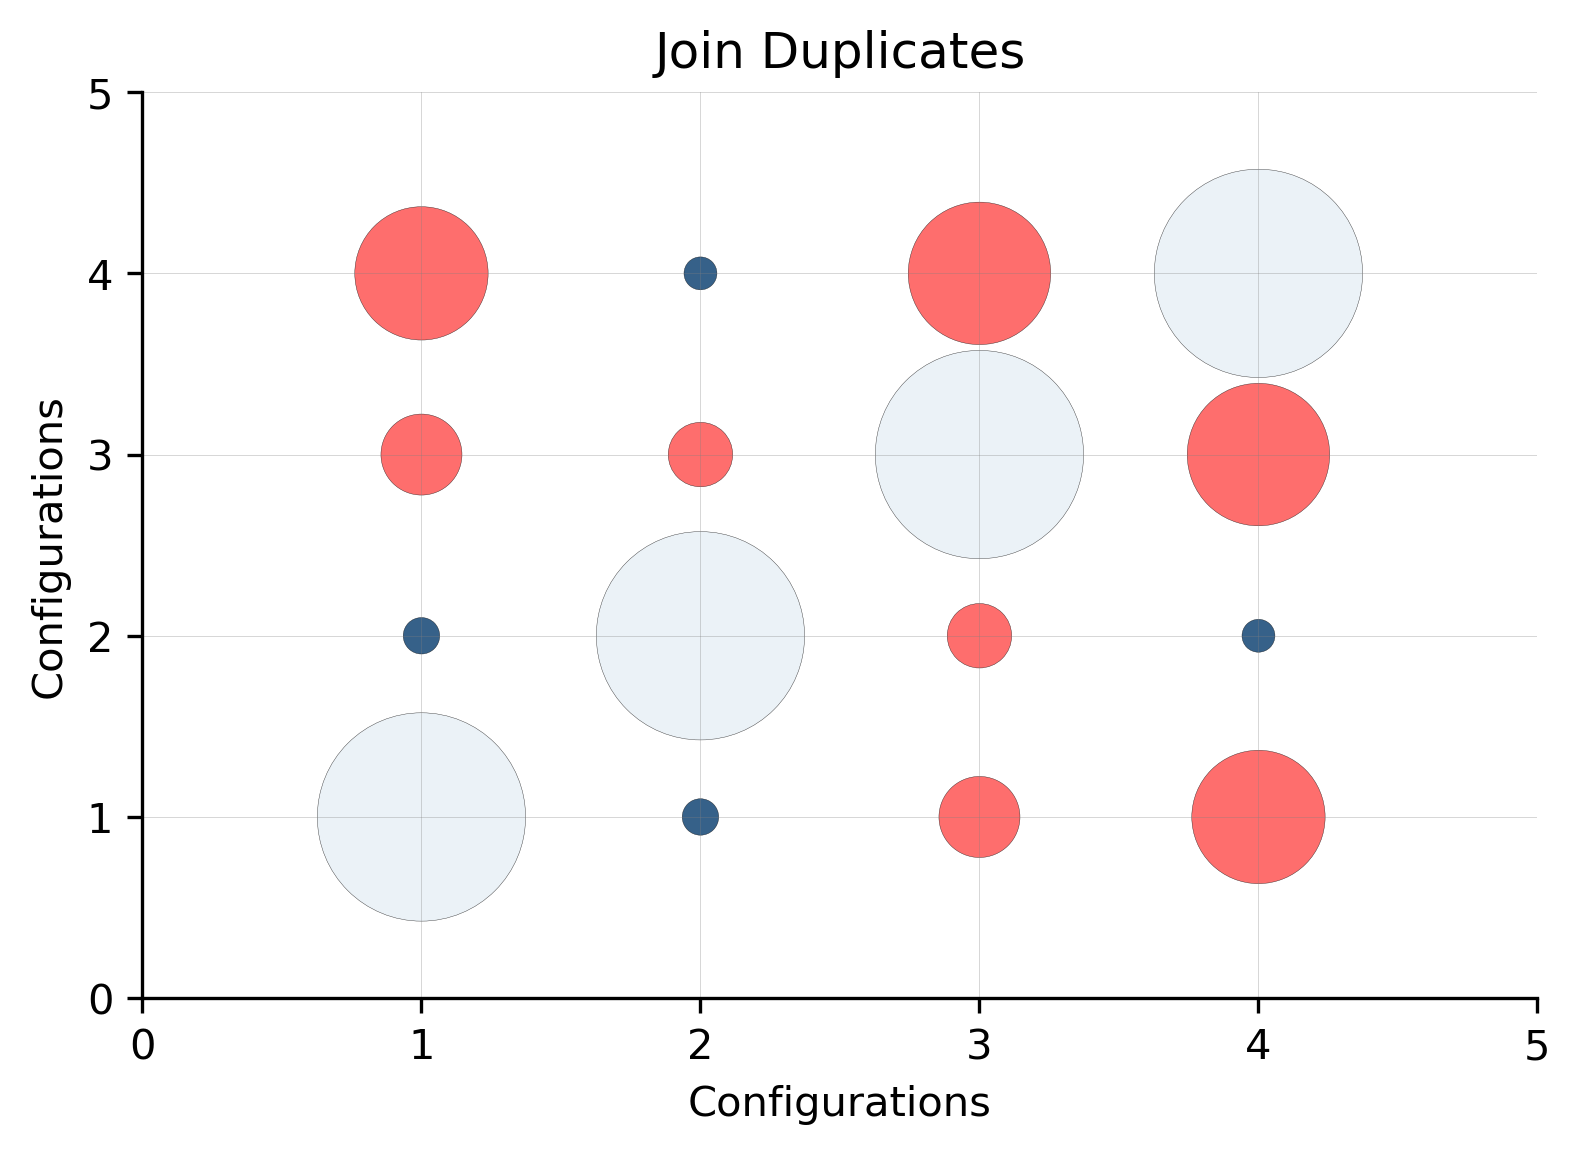
\includegraphics[width=0.48\columnwidth]{figures/duplicate_joins_01k_bubble.png}
      \label{fig:naive1}
    }
    \subfloat[Dataset 10K]{
      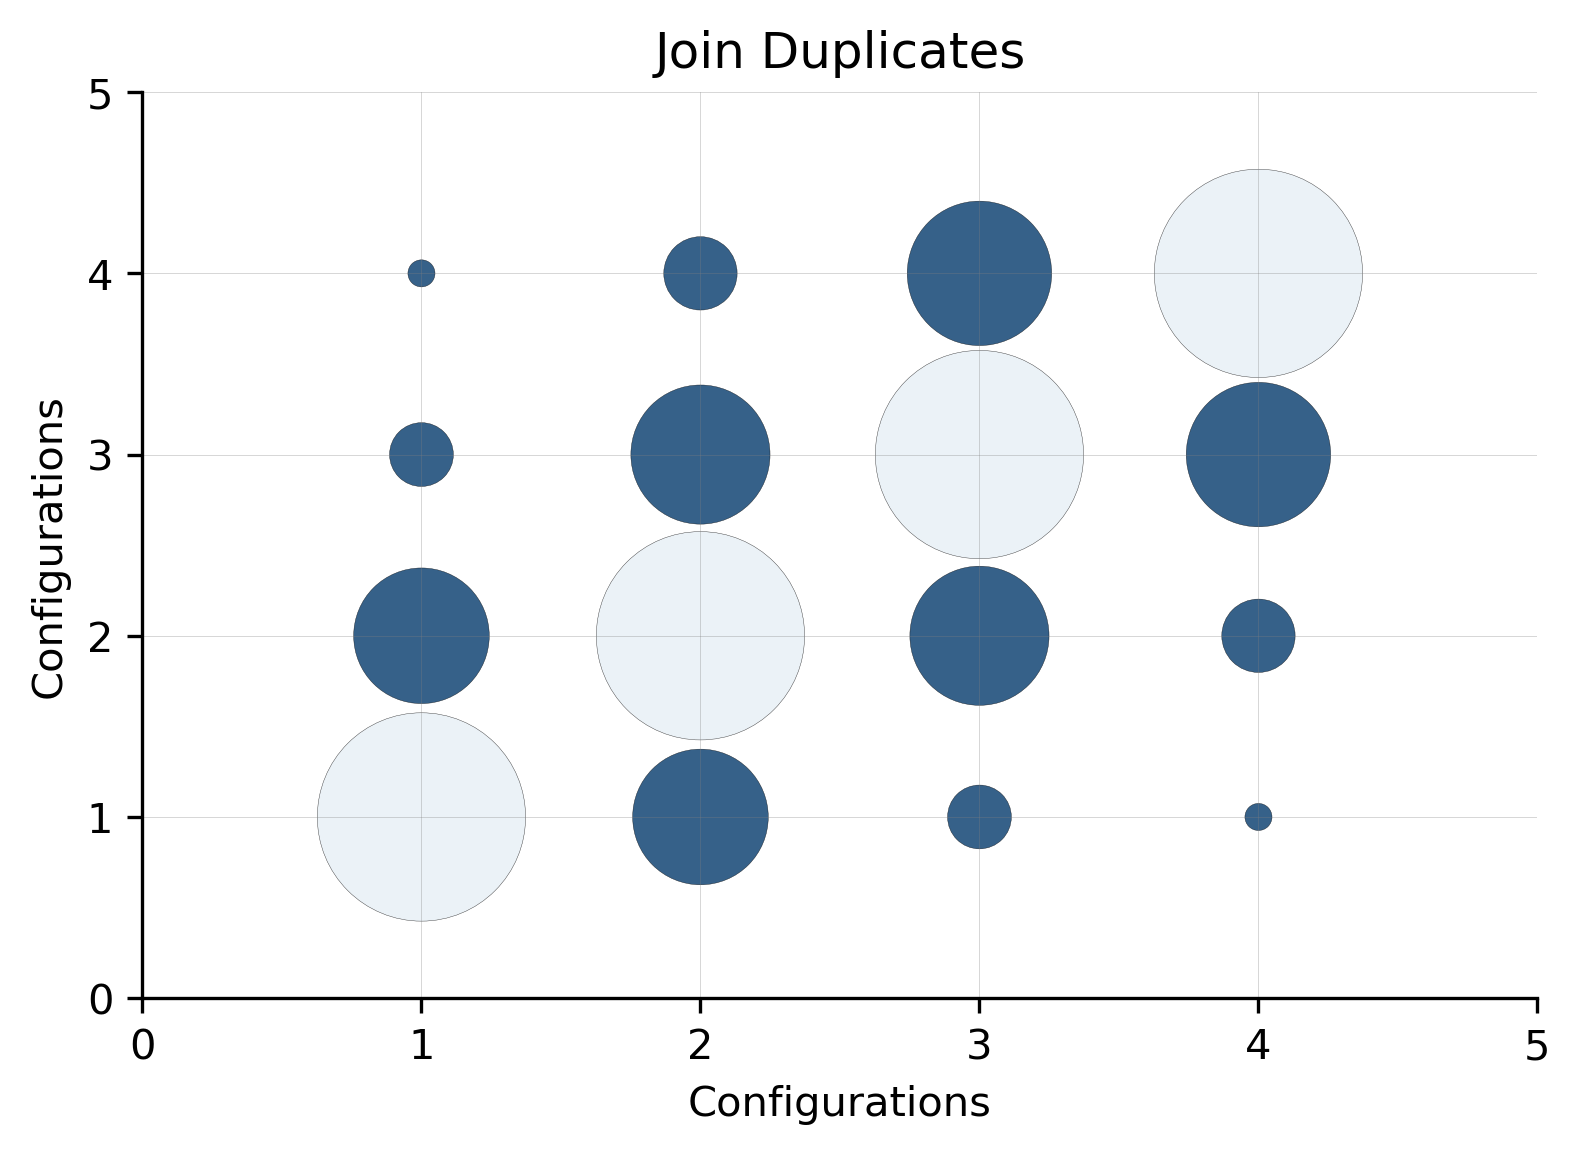
\includegraphics[width=0.48\columnwidth]{figures/duplicate_joins_10k_bubble.png}
      \label{fig:js0}
    }
    \qquad
    \subfloat[Dataset 50K]{
      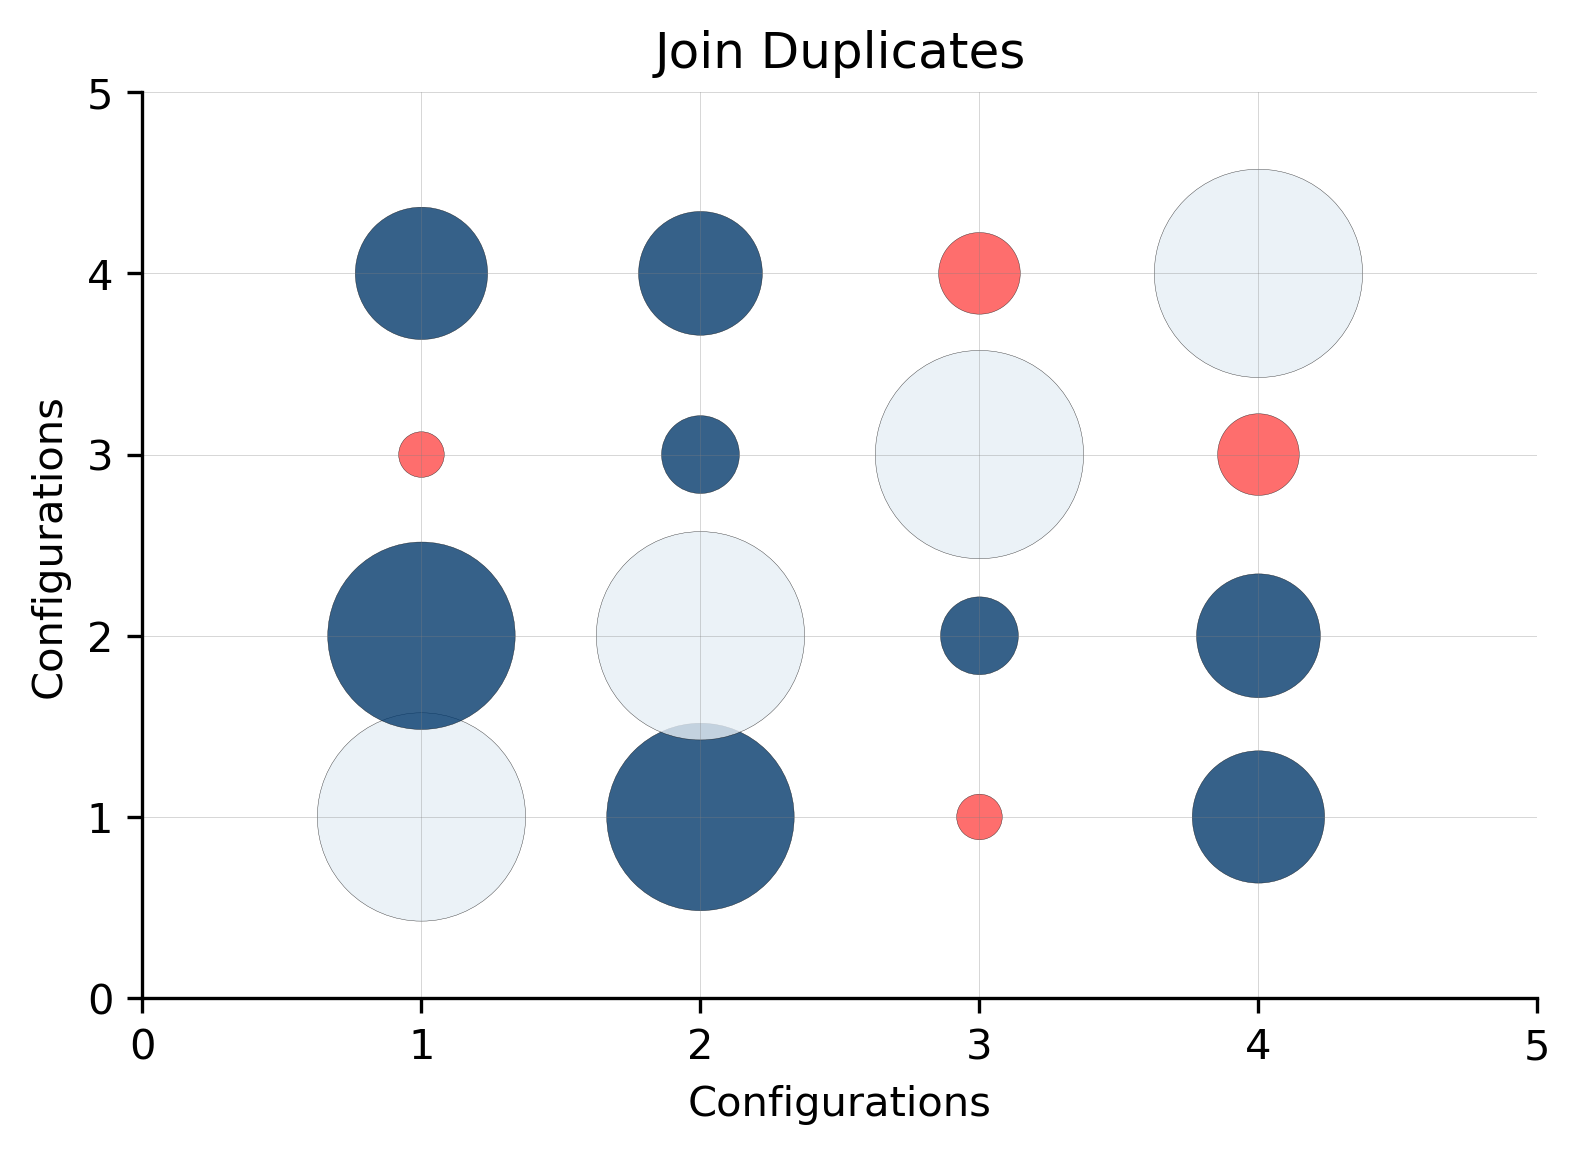
\includegraphics[width=0.48\columnwidth]{figures/duplicate_joins_50k_bubble.png}
      \label{fig:naive2}
    }
    \subfloat[Combination of 1K, 10K, and 50K]{
      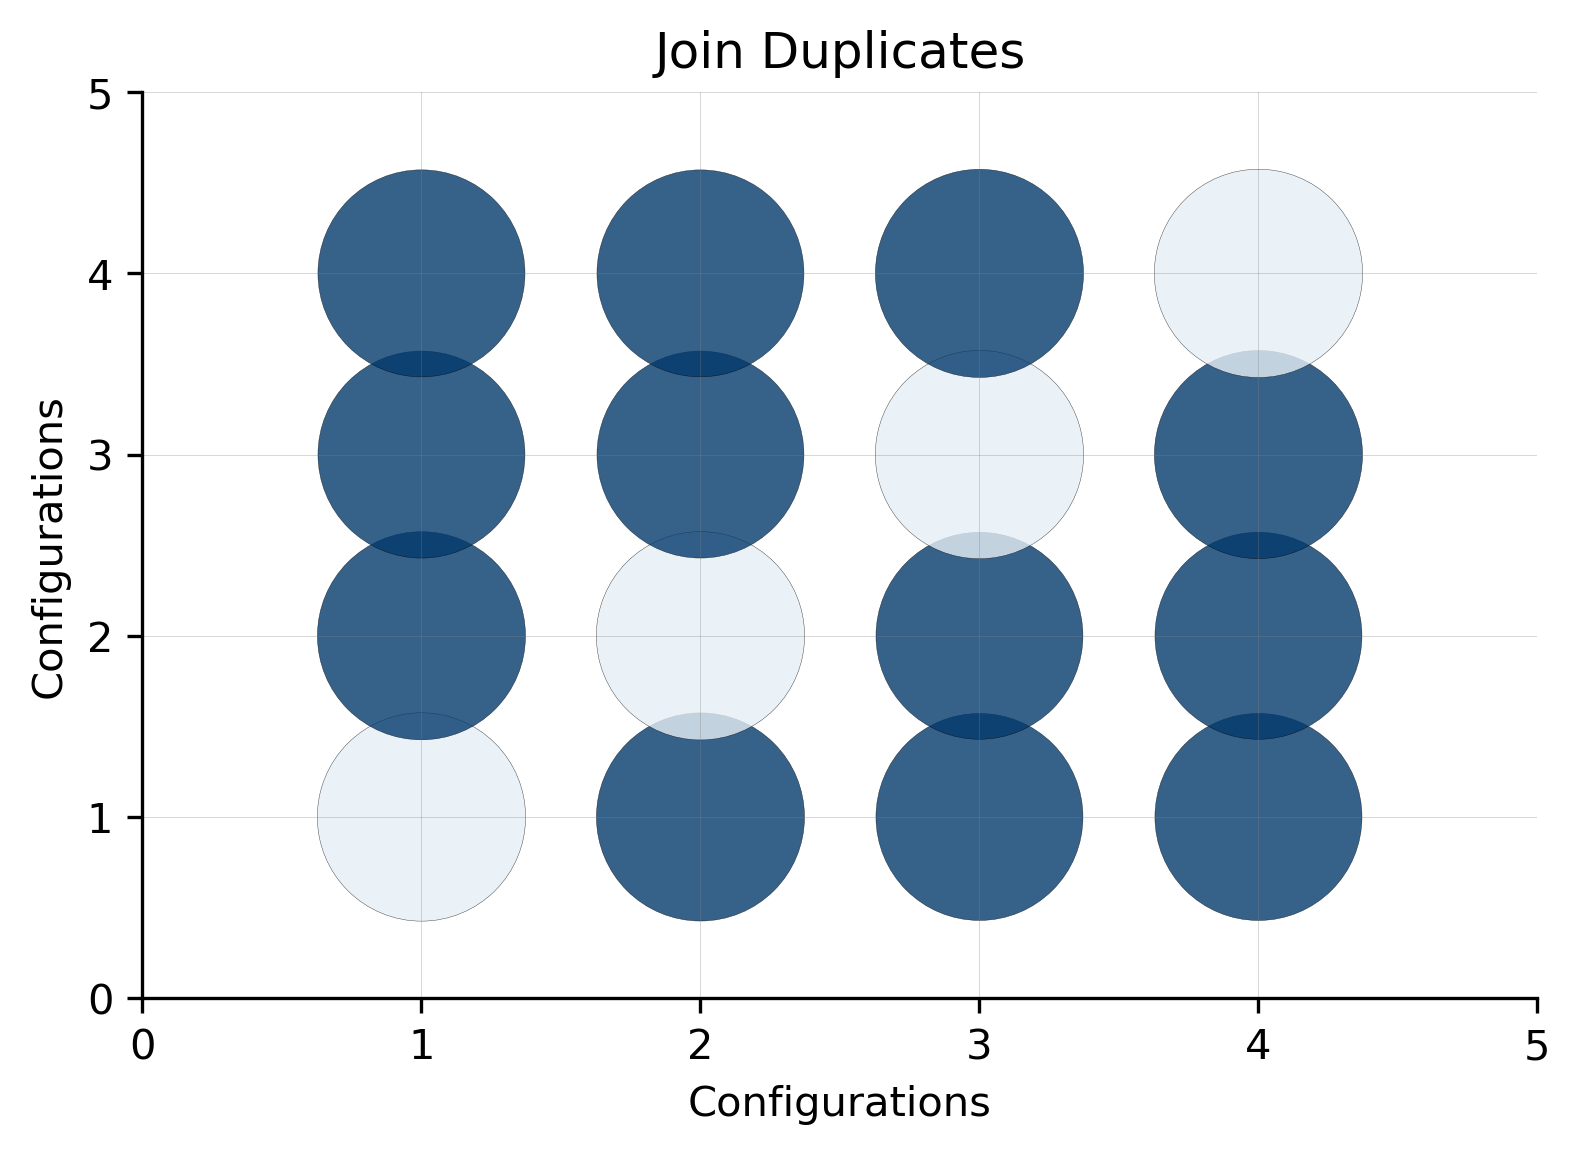
\includegraphics[width=0.48\columnwidth]{figures/duplicate_joins_allk_bubble.png}
      \label{fig:js1}
    }
    \caption[Knowledge Graph Construction Tools on Duplicates during Join]{\textbf{Comparison of Knowledge Graph Construction Tools on Duplicates during Join.} The first two (2) configurations, i.e., 1-2 on x-axis and y-axis, represent results of SDM-RDFizer on datasets with \textit{low} (5\%-20\% of data) number of duplicates and \textit{high} (30\%-50\% of data) number of duplicates generated during joins, respectively. The last two configurations, i.e., 3-4 on x-axis and y-axis, represent results of RMLMapper on datasets with \textit{low} number of duplicates and \textit{high} number of duplicates generated during joins, respectively. Grey bubbles correspond to correlation value of $1.0$; blue bubbles show a positive correlation while red bubbles show a negative correlation. Results evidence that both join duplicates and dataset size are needed for characterising an engine performance.}
    \label{fig:duplicates_bubble}
\end{figure}


\begin{figure}[!tb]
    \centering
    \subfloat[Dataset 1K]{
      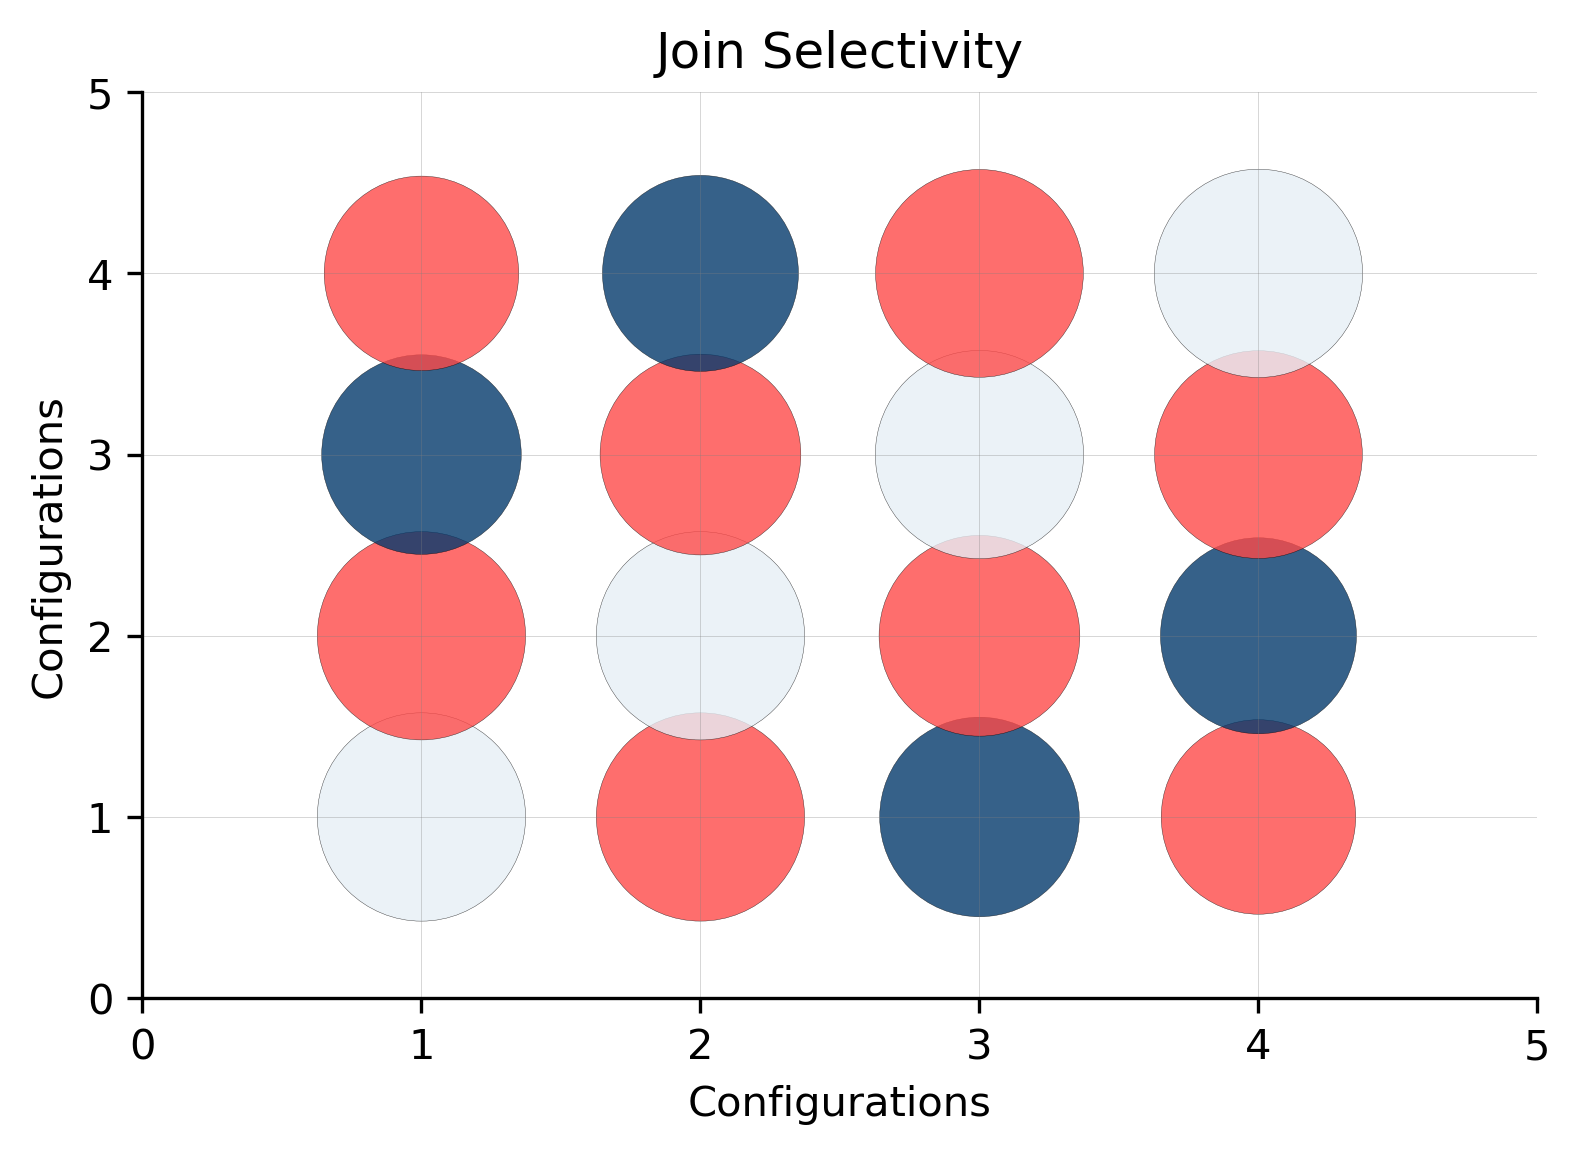
\includegraphics[width=0.48\columnwidth]{figures/join_selectivity_01k_bubble.png}
      \label{fig:naive3}
    }
    \subfloat[Dataset 10K]{
      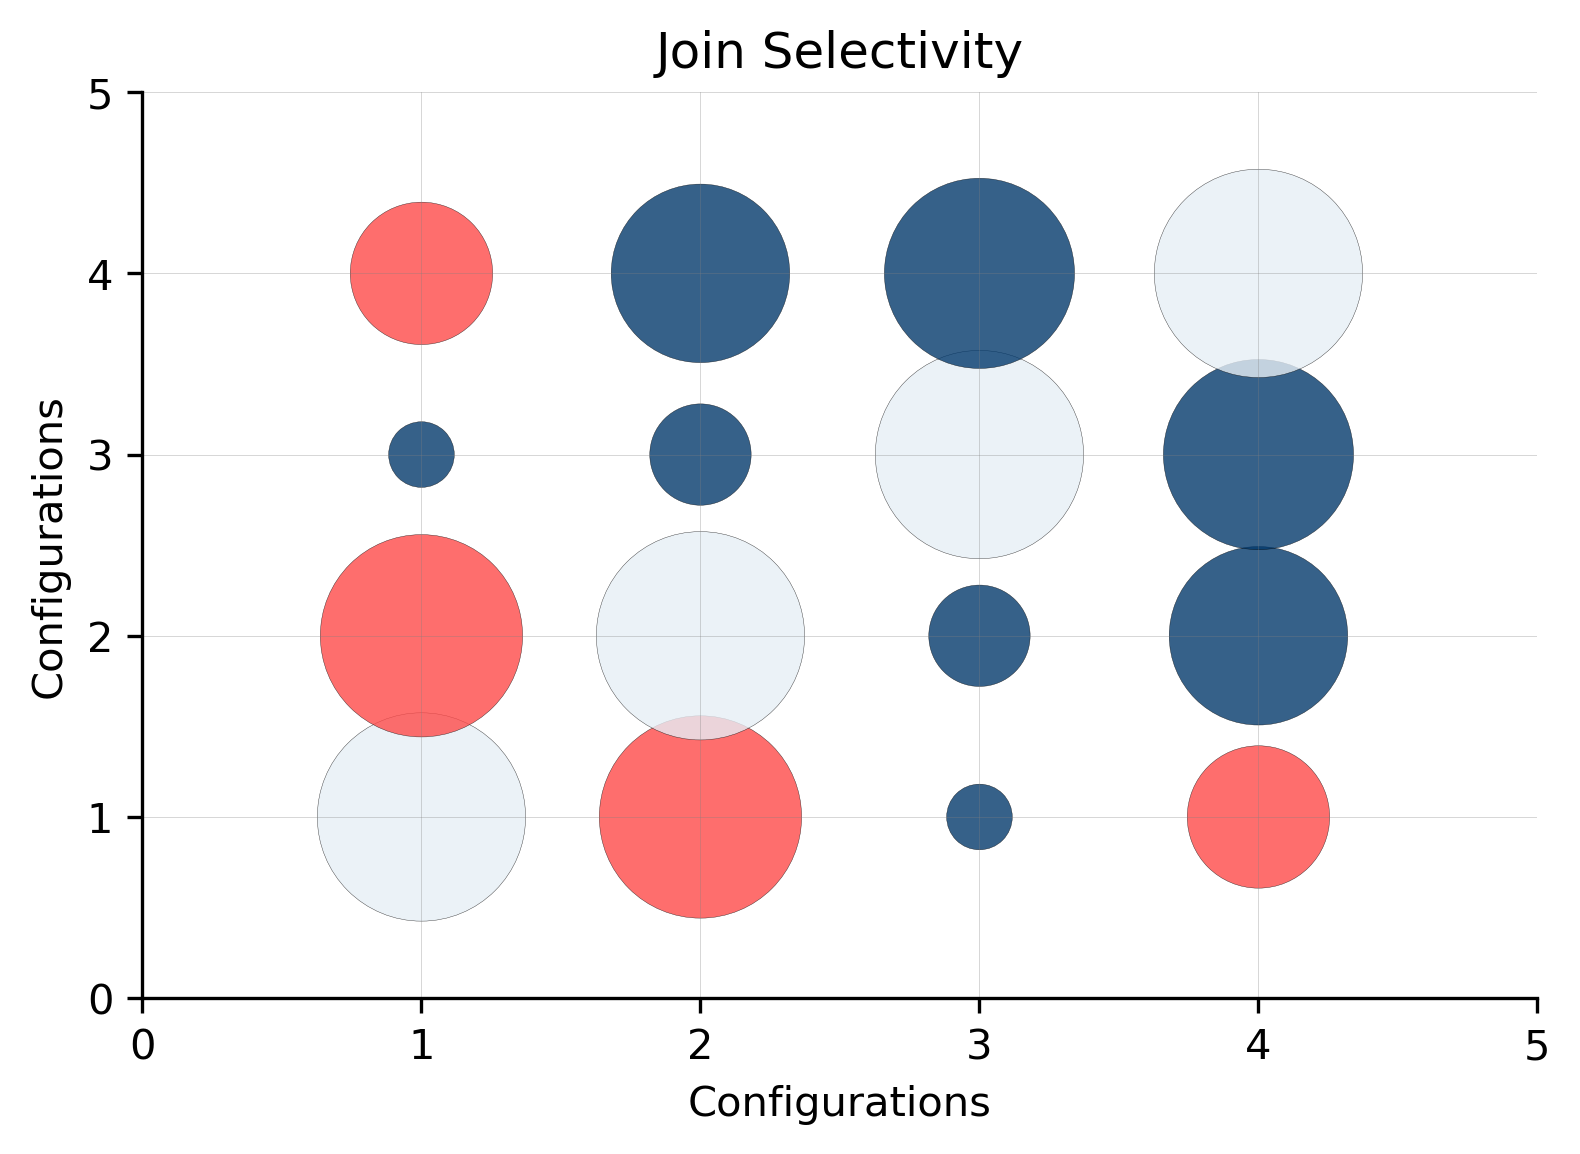
\includegraphics[width=0.48\columnwidth]{figures/join_selectivity_10k_bubble.png}
      \label{fig:js3}
    }
    \qquad
    \subfloat[Dataset 50K]{
      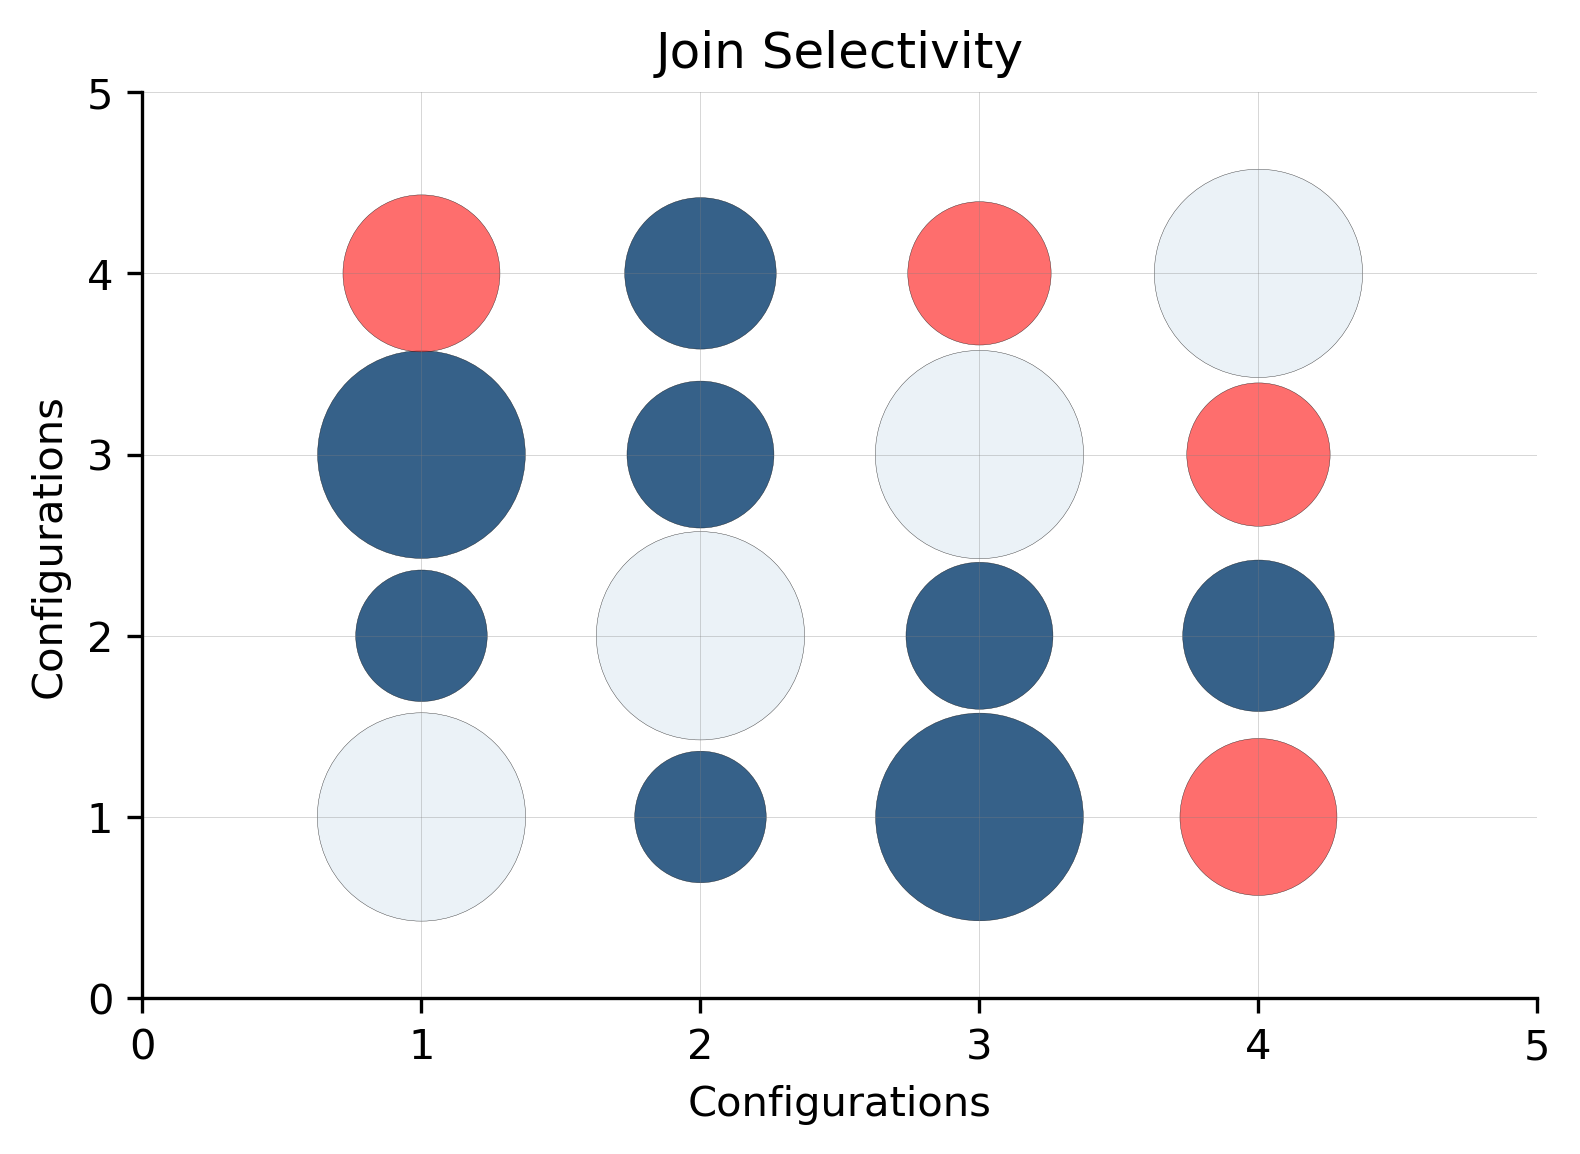
\includegraphics[width=0.48\columnwidth]{figures/join_selectivity_50k_bubble.png}
      \label{fig:naive4}
    }
    \subfloat[Combination of 1K, 10K, and 50K]{
      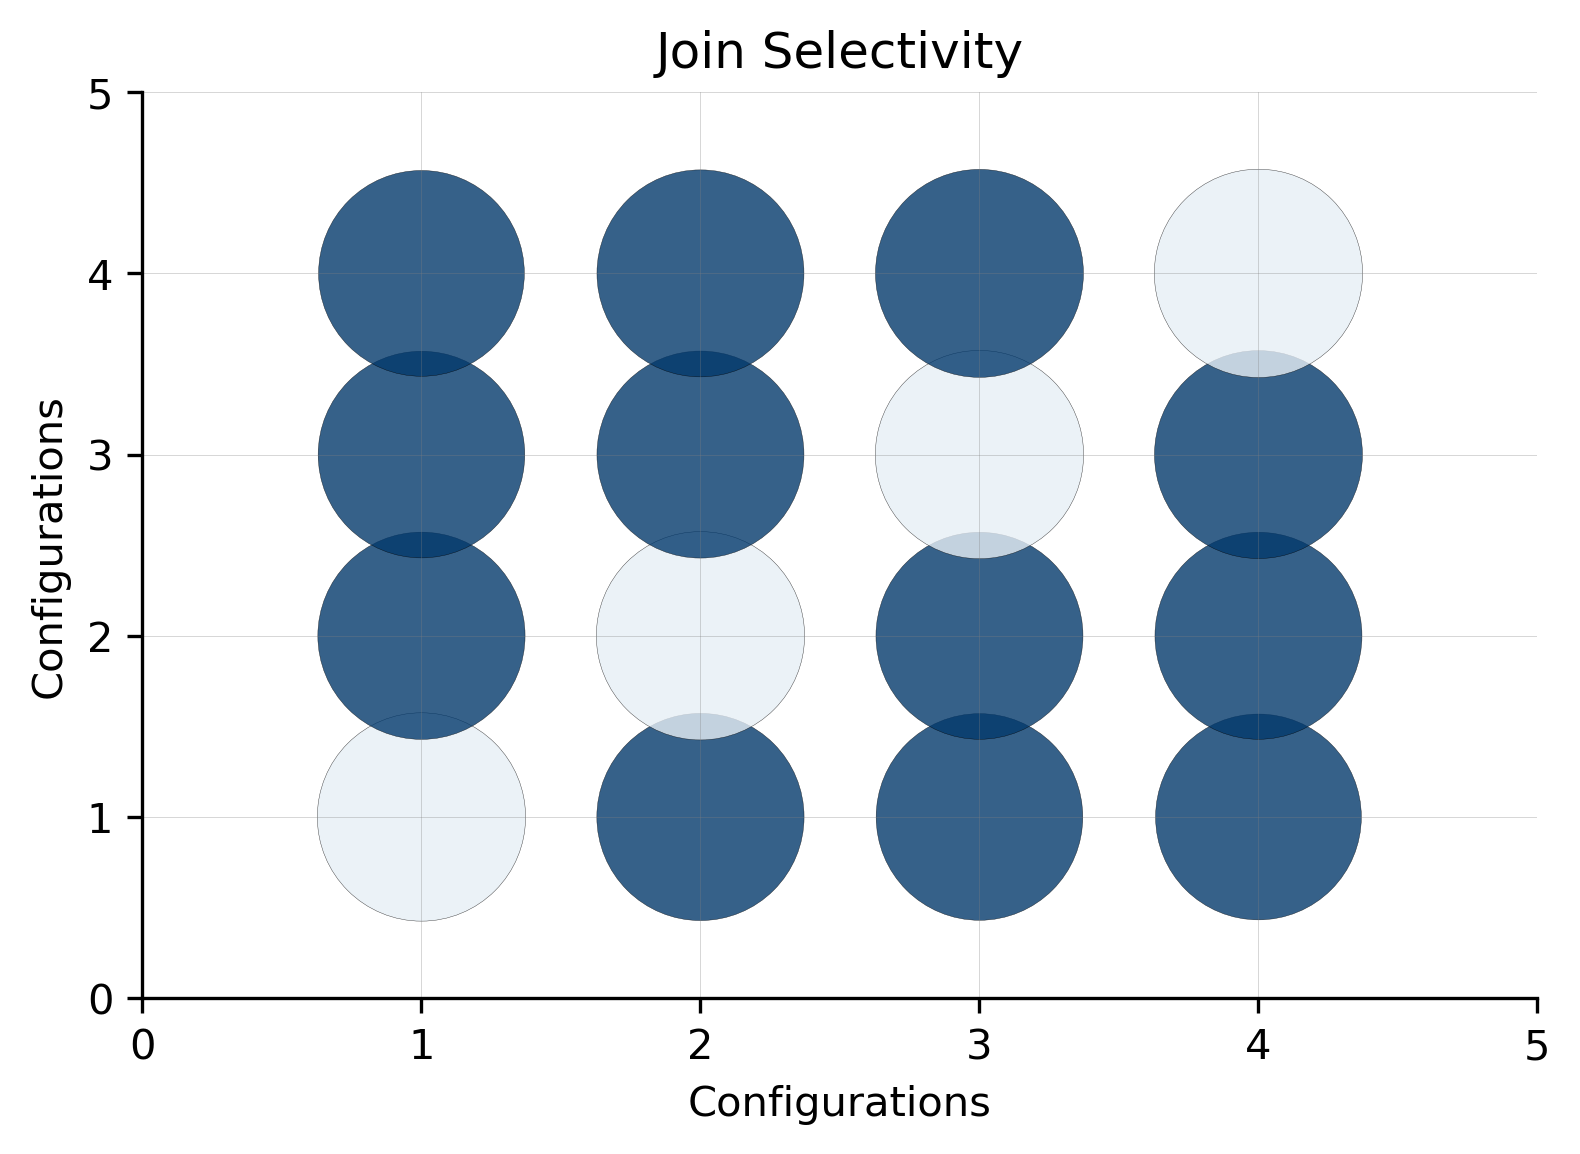
\includegraphics[width=0.48\columnwidth]{figures/join_selectivity_allk_bubble.png}
      \label{fig:js4}
    }
    \caption[Knowledge Graph Tools on Join Selectivity]{\textbf{Comparison of Knowledge Graph Tools on Join Selectivity.} The first two configurations, i.e., 1-2 on x- and y-axis represent SDM-RDFizer on joins with \textit{high} selectivity (5\%-20\% of data) and joins with \textit{low} selectivity (60\%-100\% of data), respectively.  Configurations 3 and 4 represent RMLMapper on joins with \textit{high} selectivity (5\%-20\% of data) and joins with \textit{low} selectivity (60\%-100\% of data), respectively. Grey bubbles correspond to correlation value of $1.0$; blue bubbles show a positive correlation while red bubbles show a negative correlation. Dataset size and join selectivity affect both engines differently.}
    \label{fig:joinselectivity_bubble}
\end{figure}



\noindent \textbf{Relation Types:}
Figure~\ref{fig:relation_type_bubble} reports on the correlation of different configurations for various join relation types. We can observe in Figures \ref{fig:rt_1k}, \ref{fig:rt_10k}, and \ref{fig:rt_50k} several red bubbles, indicating a negative correlation in the behavior of the compared configurations and engines. Contrary, Figure \ref{fig:rt_all} does not depict any red bubble, suggesting thus, that the two engines in all the configurations exhibit the same behavior. These results clearly illustrate the need of considering different configurations and parameters in order to avoid drawing wrong conclusions about the main characteristics of existing tools. 


\noindent \textbf{Join Duplicates:}
Figure~\ref{fig:duplicates_bubble} depicts the correlation between different configurations when different setting of duplicates are produced during the execution of joins between triple maps. As can be observed, Figures \ref{fig:naive1}, and \ref{fig:naive2} include several red bubbles that indicate an opposite behavior of the engines. Contrary, Figures \ref{fig:js0}, and \ref{fig:js1} suggest that both engines behave similarly. 


\noindent \textbf{Join Selectivity:}
Figure~\ref{fig:joinselectivity_bubble} shows the correlation between different configurations for the selectivity of join conditions. Similarly, these testbeds reveal contradicting patterns in the behaviors of the studied engines. On one hand, Figures \ref{fig:naive3}, \ref{fig:js3}, and \ref{fig:naive4} are composed of several red bubbles and indicate that these engines perform differently whenever the selectivity of the join condition is changed. Surprisingly,  when the size of these datasets are also taken into account in the testbed (Figure \ref{fig:js4}), these patterns are hidden, and the results of the evaluation suggest that both engines perform similarly whenever the selectivity of the join condition is changed. 

The results reported in this experimental study provide clear evidence of the importance of the variables and configurations that composed the methodology devised in this work. Actually, in the four studied cases, they reveal important patterns that could not be observed whenever other parameters were studied simultaneously. Based on these observations, we can conclude that these variables and configurations should be included in the benchmarks in order to ensure that the characteristics of knowledge graph construction engines are uncovered. Thus, these observations allow us to answer our three research questions: \textbf{RQ1}, \textbf{RQ2}, and \textbf{RQ3}. We encourage developers and users of knowledge graph construction tools to bear in mind them during benchmarking in order to draw clear conclusions about the performance of their tools.


\subsection{Conclusions}
In this section, we performed an in-depth analysis of the variables and configurations that impact on the behavior of two engines. The observation that existing engines exhibit heterogeneous behaviors whenever small changes in the testbeds are conducted, motivated the need of conducting this study involving a set of parameters that can reveal patterns in the behavior of the studied engines. Additionally, the lack of testbeds encouraged us to acquit the definition of variables and configurations that enable for the characterization of the pitfalls of existing engines and for identifying the list of challenges and research directions in the state of the art. 
With the proposed analysis and the results of the experimental study, we contribute with an empirical configuration that can be reused for the evaluation of other knowledge graph construction tools and mapping languages (e.g., SPARQL-Generate, TARQL, or R2RML). Furthermore, our set of variables and configurations can be utilized as a guideline during testing and benchmarking. One of the main lessons learned during the definition and evaluation of our approach, is that none of the evaluated engines behaves consistently whenever the complexity of the testbeds increases. Our ambition is that the reported results inspire the community to define general testbeds that facilitate the understanding of the state of the art and the development of novel tools for the construction of knowledge graphs at large scale.  In the future, we plan to define testbeds and conduct a more detailed analysis of other engines and mapping languages. Moreover, we envision to motivate the community to conduct a joint effort in the definition of benchmarks that enable for fair evaluations of knowledge graph construction tools with replicable and generalizable results. 


\section{GTFS-Madrid-Bench: Evaluation of Virtual Knowledge Graph Access}

%Over the last few years, a growing number of datasets have been made available in various open data portals. For example, the European Data Portal\footnote{https://www.europeandataportal.eu/catalogue-statistics/CurrentState} aggregates, at the time of writing, approximately 500K datasets from EU countries in a diversity of domains. In this context, RDF has been proposed as a standard format for data interchange on the Web, and RDF Schema and OWL ontologies have begun to appear so as to provide shared models in some domains. However, the amount of non-RDF data (e.g., CSV, JSON, XML) that is published in these open data portals continues to dominate the scene (see Table \ref{tab:odp}) and interoperability issues hinder their (re)use and consumption. 

%Data integration is not a new problem but it is exacerbated by the availability of such open data on the Web, that is, it was already identified and addressed several decades ago with an emphasis on data in relational databases. Different techniques and tools have been used to address this problem. In our work, we focus on those based on ontologies. In Ontology Based Data Access (OBDA)~\citep{poggi2008linking} data consumers issue queries over a dataset according to a common unified view (an ontology). The information needed to reformulate the queries is usually available in the form of declarative mappings. In Ontology Based Data Integration (OBDI)~\citep{poggi2008linking}, these techniques are expanded to address heterogeneous datasets, whose data needs to be integrated to provide answers to these queries. In both ontology-based approaches, two different alternatives exist to enable data access: (1) those where data are materialised taking into account the mappings and the ontologies (for example, data is transformed into RDF and loaded into a triple store, so that it can be queried using SPARQL), and (2) those where the transformation is done on the queries, which can then be evaluated on the original data sources. This last alternative is the one considered for our work because it removes the need for materialisation, something especially useful for very dynamic data sources~\citep{corcho2019towards}. We refer to it as ``virtualized knowledge graph access''.

%To facilitate data exploitation in this context, application developers need to understand the strengths and weaknesses of existing data integration tools. Additionally, tool developers may want to know if their engines cover the requirements of real use-case scenarios. In both cases the challenge is to develop a benchmark that covers the requirements of ``virtualized knowledge graph access''  and that is extensible and sustainable over time. In general, it is  necessary to have an overview of state of the art engines that are tailored to different source formats, accepting as input mappings that are represented in a variety of declarative languages.

%Several benchmarks already exist in the state of the art of OBDA~\citep{bizer2009berlin,lanti2015npd}, as well as in SPARQL query federation~\citep{schmidt2011fedbench,hasnain2017biofed,montoya2012benchmarking}. The OBDA BSBM benchmark~\citep{bizer2009berlin} is focused on comparing the performance of SPARQL-to-SQL query translation versus the performance of native RDF Stores, and only considers OBDA engines that access relational data stores. The NPD benchmark~\citep{lanti2015npd} specifically analyzes OBDA requirements related to datasets, query sets, mapping rules and query languages. In the area of federated SPARQL engines, existing benchmarks~\citep{schmidt2011fedbench,hasnain2017biofed,montoya2012benchmarking} are tailored to the context of SPARQL endpoint federation in an homogeneous format. As a result, none of these benchmarks address the requirement of virtualized access of multiple datasets available in heterogeneous formats. Additionally, OBDI engines have been evaluated in an ad-hoc manner ~\citep{endris2019ontario,mami2019querying} and to the best of our knowledge, no benchmarks have been developed to evaluate OBDI proposals in a systematic manner. 

We have identified several challenges for the development of a benchmark for virtual knowledge graph access that can be grouped into data, queries and mappings dimensions. The data challenges refer to having multiple data sources in an assortment of formats based on real-world data, and that can scale to large sizes. The challenges referred to queries point to SPARQL queries where different sources can be identified, where relations among sources (according to the specific data model) are exploited, and where necessary features of SPARQL are included to represent real-life use cases. Finally, the main mappings challenge is to include the relevant parameters that affect in the generation of the virtual knowledge graph~\citep{chaves2019what} and give support to a set of declarative mapping languages.

To address these challenges, in this section, we describe a ``virtual knowledge graph access'' benchmark, GTFS-Madrid-Bench, that serves several purposes: (i) to evaluate and compare the performance of a mix of KGC engines that access several (homogeneous) sources in the same format, but where the mapping language used by each engine is specific to the data format considered; (ii) to evaluate virtual KGC engines over heterogeneous data sources; and (iii) to evaluate the strengths and weaknesses of both approaches. The general case of GTFS-Madrid-Bench is the comparison of the performance of KGC engines. The proposed GTFS-Madrid-Bench is composed of the following elements:

%\begin{table}
%\centering
%\caption[Caption]{Most commonly used formats (and percentage over the total number of datasets) to publish data in mature EU open data portals\footnotemark}
%\label{tab:odp}
%\resizebox{0.48\textwidth}{!}{
%\begin{tabular}{c|c|c|c}
%\hline
%\textbf{Data Portal} & \textbf{1st Format}  & \textbf{2nd Format} & \textbf{3rd Format} \\ %\hline
%Spain                & CSV (50\%)  & XLS (35\%)  & JSON (33\%)          \\ 
%Norway               & CSV (77\%)    & GEOJSON (17\%)         & JSON (14\%)            \\ 
%Italy               & CSV (76\%)  & JSON (35\%)          & XML (25\%)           \\ 
%Croatia              & XLS (63\%)    & CSV (40\%)   & HTML (33\%)           \\ 
%Luxembourg              & ZIP (25\%)    & CSV (24\%)   & PDF (18\%)           \\ 
%Ireland              & JSON (49\%)    & CSV (39\%)   & TXT (22\%)           \\\hline
%\end{tabular}
%}
%\end{table}
%\footnotetext{Statistics obtained in January 2019 (note that one dataset can be made available in multiple formats)}

\begin{itemize}
    \item Several collections of sources in different formats (e.g. CSV, JSON, SQL, XML), which derive from the GTFS\footnote{The General Transit Feed Specification (GTFS) is a de-facto standard developed by Google for the description of public transport planning, routes and fares, among others. In recent years its popularity has increased thanks to its simplicity and the fact that it has not only been adopted by Google Maps, but also by other route planning systems such as Open Trip Planner or navitia.io.: \url{https://developers.google.com/transit/gtfs/}} feed from the metro of the city of Madrid. These collections are scaled up so as to allow scalability testing.
    \item A set of mappings represented in the family of declarative languages that address different source formats (RML, R2RML, xR2RML, ontop OBDA mappings) that map the GTFS-based data sources into the Linked GTFS ontology\footnote{\url{https://github.com/OpenTransport/linked-gtfs}}.
    \item A set of 18 SPARQL queries of varied complexity.
    \item A set of well-established measurements~\citep{mora2013towards,lanti2015npd} that can be taken during the different phases of the KGC workflow~\citep{lanti2015npd,acosta2011anapsid}, such as query rewriting, query translation, query execution and query aggregation time.
\end{itemize}
GTFS-Madrid-Bench offers a fair environment for the comparison of different KGC engines, regardless of the mapping language that they have implemented, as long as the new mappings follow the same restrictions and specifications defined in the benchmark. Thus, newly released tools may be evaluated with the benchmark. Additionally, although we have generated our datasets from the GTFS feed of the city of Madrid metro system, any other city's GTFS feed may be used as data in the benchmark. 

We provide a data generator to scale up the original data in terms of size, and distribute the datasets over different formats (e.g. JSON, XML, CSV, RDB). We demonstrate the use of GTFS-Madrid-Bench with five open source engines: Morph-RDB\footnote{\url{https://github.com/oeg-upm/morph-rdb}}, Ontop\footnote{\url{https://github.com/ontop/ontop}}, Ontario\footnote{\url{https://github.com/SDM-TIB/Ontario}}, Morph-CSV\footnote{\url{https://github.com/oeg-upm/morph-csv}} and Morph-xR2RML\footnote{\url{https://github.com/frmichel/morph-xr2rml}}. 

In summary, the main contributions of this work are:
\begin{enumerate}
    \item C1: The proposal of a comprehensive and representative benchmark that includes a set of data sources, queries and mappings that allow evaluating and comparing multiple KGC engines for virtual knowledge graph access.
    \item C2: The extension of existing OBDA benchmark requirements to take into account (i) metrics that are commonly used in federated query processing benchmarks; and (ii) steps defined in new KGC engines~\citep{corcho2019towards}.
    \item C3: A data generation process where single and mixed data formats are scaled-up based on the features of the original data model, integrating state of the art data generator proposals for benchmark OBDA engines~\citep{lantivig}.
    \item C4: Evaluation of the proposed benchmark over five different engines, discussion of the obtained results and identification of the current limitations in the state of the art and future lines of work. 
\end{enumerate}


\subsection{Preliminaries}

In this section, we introduce the main concepts and definitions that are later used to explain our work. Besides this, well-known concepts from the literature such as SPARQL queries and result sets~\citep{w3c2013sparql}, or ontologies~\citep{mcguinness2004owl} will be used throughout this work.

\paragraph{\textbf{Sources \& Dataset:}} we define a source as a tuple $\gamma=(\varphi,$ $\Sigma ,$ $f)$ where $\varphi$ is the data of any entity from our domain, $\Sigma$ is the model of the data, e.g. the columns of a CSV or the schema of a database table for SQL, and $f$ is a specific data format such as CSV, JSON, XML, or SQL, among others.% Remove this to go back to previous version
~ We define a dataset as a set of \textit{Sources}, i.e., $\mathcal{D}=\{\gamma_1,\gamma_2, ..., \gamma_n\}$. 

\textit{Example 1.} We define the following dataset $\mathcal{D}_{1}=\{(Rou\-tes,$ $\Sigma_1,$ $SQL),$ ($Stops,$ $\Sigma_2,$ $JSON)\}$ that involves the data of the metro routes (13 instances) and metro stops (1262 instances) in SQL and JSON formats, respectively. Both sources rely on different schemata $\Sigma_1$ and $\Sigma_2$, the first specifies the columns of a table and the second the keys of a JSON.

\paragraph{\textbf{Dataset Generator:}} we define a dataset generator as a function $\delta$ that takes as input a tuple ($\mathcal{D}$, $s$) where  $\mathcal{D}$ is a dataset and $s$ is a non-negative number that specifies a scale factor. The output of $\delta$ is a dataset $\mathcal{D'}$ containing enlarged versions, according to $s$, of the data ($\varphi$) within the sources of $\mathcal{D}$.

\textit{Example 2.} Assuming $\mathcal{D}_{1}$ from \textit{Example 1} and a scale factor $s$ of 2.5, a dataset generator may produce the following $\mathcal{D'}=\{(Rou\-tes{-}2.5,$ $\Sigma_1,$ $SQL),$ ($Stops{-}2.5,$ $\Sigma_2,$ $JSON)\}$. Notice that the schematas and the formats are the same, but the data of $Rou\-tes\-2.5$ and $Stops\-2.5$ has been scaled up from their versions in $\mathcal{D}_{1}$, containing 189 and 3536 instances respectively.

\paragraph{\textbf{Mapping:}} a mapping $m$ is a set of rules that specify the relationship between an ontology and the model of one or more sources. A mapping rule relates the elements within the schema of a source with elements from an ontology, including constants. In other words, a mapping rule $r$ contains the correspondences between an element $e$ within a schema of a source $\Sigma$ and an element $e_*$ of an ontology $\Sigma_*$. The ontology is known as unified view since it is the output of translating heterogeneous sources into the same model, i.e., the ontology.

\textit{Example 3.} Given the LinkedGTFS ontology and a CSV file with the columns ``id'' and ``route'', a mapping may state that each row generates a subject that includes the value of the column ``id', the predicate \textit{foaf:name} and its object with the corresponding value in the column ``route''.

\paragraph{\textbf{Experiment configuration:}} we define an experiment configuration $c$ as $(\mathcal{D}, q, M)$ where $\mathcal{D}$ is a dataset, $q$ is an SPARQL query and $M$ is a set of mappings.

\textit{Example 4.} We can specify the following experiment configuration $(\mathcal{D}_{1}, q1, \{shapes, trips\})$, where $\mathcal{D}_{1}$ is the data\-set specified in \textit{Example 1}, $q_1$ is the SPARQL query reported in Table~\ref{tab:queries}, 
and $M$ is the set of mappings $\{shapes, trips\}$  reported in Table~\ref{tab:mappings}.

\paragraph{\textbf{Processor:}} Given an experiment configuration $c$ and an ontology $\Sigma_*$, a processor represents a software component that encodes the function $\phi$ that takes as input a pair  $(c,\Sigma_*)$ and outputs a SPARQL result set $R$ ~\citep{w3c2013sparql}. 

Internally, the processor translates the SPARQL query $q$ into one or more queries expressed in different languages, depending on the formats within the dataset of $c$, using the mappings $M$. Then, the processor distributes and evaluates the queries and gathers the results. As a result, a unified result set is provided as output. This task is known as \textbf{Virtual Knowledge Graph Access}. We distinguish two kinds of processors: OBDA and OBDI. The former ones are able to handle only experiment configurations where all the data sources have the same data format. The latter ones are able to handle any experiment configuration.



\subsection{Benchmark Proposal}

% Introduction
%The General Transit Feed Specification (GTFS) is a \textit{de-facto standard} developed by Google for the description of public transport schedules, routes, fares, etc. Recently, it has become popular due to its simplicity, and due to the fact that it has been adopted not only by Google Maps, but also by other route planning systems such as \textit{Open Trip Planner}, or \textit{Navita.io}. The specification defines the headers of 13 types of CSV files and a set of rules. Each file, as well as their headers, can be mandatory or optional and they have relations among them.
\begin{table}[]
\caption{Virtual Knowledge Graph Access Benchmark Requirements}
\label{tab:req}
%\setlength{\tabcolsep}{1em}
\resizebox{0.70\textwidth}{!}{
\begin{tabular}{c|l}
\hline
\textbf{Variable} & \multicolumn{1}{c}{\textbf{Requirement}} \\ \hline
Ontology & \begin{tabular}[c]{@{}l@{}}The \textbf{ontology} should include classes with \\ data and  object properties \end{tabular} \\ \hline
Dataset & \begin{tabular}[c]{@{}l@{}}The \textbf{virtual instance} should maintain the constraints \\ defined in the original dataset\end{tabular} \\ \hline
Dataset & The \textbf{virtual instance} should be based on real world data \\ \hline
Dataset & \begin{tabular}[c]{@{}l@{}}The \textbf{virtual instance} should be distributed\\  in different data formats\end{tabular} \\ \hline
Mappings & \begin{tabular}[c]{@{}l@{}}The \textbf{mappings} should be able to indicate\\the format of the source\end{tabular} \\ \hline
Mappings & \begin{tabular}[c]{@{}l@{}}The \textbf{mappings} should be expressed\\using well known mapping languages\end{tabular} \\ \hline
Queries & The \textbf{query set} should be based on actual user queries \\ \hline
Queries & \begin{tabular}[c]{@{}l@{}}The \textbf{query set} should be complex enough with \\ relations among same but also different data sources\end{tabular} \\ \hline
Metrics & \begin{tabular}[c]{@{}l@{}}The \textbf{metrics} should provide relevant general information \\ but also specific measures for each defined phase\end{tabular} \\ \hline
\end{tabular}}

\end{table}


The GTFS-Madrid Benchmark consists of an ontology, an initial dataset of the metro system of Madrid following the GTFS model, a set of mappings in several specifications, a set of queries according to the ontology that cover relevant features of the SPARQL query language, a data generator based on a state of the art proposal~\citep{lantivig}, and a set of relevant metrics. In the following sections we describe in detail the resources of our virtual knowledge graph access benchmark. They are aligned with an extension of the requirements detailed in~\citep{lanti2015npd} (focused on benchmarks for OBDA) that we tailor to our context (Table \ref{tab:req}). All the resources described in this section are available online\footnote{\url{https://github.com/oeg-upm/gtfs-bench}}.

\subsubsection{The Linked GTFS Ontology} 
GTFS is a \textit{de-facto standard} developed by Google for the description of public transport schedules, routes, fares, etc. The specification defines the headers of 13 types of CSV files and a set of rules. Each file, as well as their headers, can be mandatory or optional and they have relations among them.

The Linked GTFS vocabulary\footnote{\url{https://github.com/OpenTransport/linked-gtfs}} can be seen as an ontology that represents the entities, properties and relationships described in the GTFS specification. The GTFS-Madrid-Bench mappings have been aligned to a subset of this vocabulary as the subway feed provides only the mandatory CSV files from the GTFS specification. Its conceptual model is shown in Figure \ref{fig:gtfsOntology} and a description of its classes is given in Table \ref{tab:GTFSClasses}. The ontology usually defines one class for each of the sources in the GTFS specification with the corresponding data and object properties, but there are some additions. The {\tt gtfs:Service} class represents information of the dates when a service (represented in GTFS in the files calendar and calendar\_dates) is available for one or more routes, the ontology also adds the {\tt gtfs:ServiceRule} class together with its two subclasses ({\tt gtfs:CalendarRule} and {\tt gtfs:CalendarDateRule})  to represent the service rules specified  in the calendar and calendar\_dates files. Finally, the class defined as \\{\tt gtfs:WheelchairBoardingStatus} and its three possible values (instances) have also been added to represent the corresponding field definitions in stops and trips. 

\begin{table}[t]
\caption{LinkedGTFS classes and their descriptions}
\label{tab:GTFSClasses}
%\setlength{\tabcolsep}{1em}
\resizebox{0.48\textwidth}{!}{
\begin{tabular}{c|l}
\hline
\textbf{Class} & \multicolumn{1}{c}{\textbf{Description}} \\ \hline
Agency & \begin{tabular}[c]{@{}l@{}} Agency that operates a certain transport mode
\end{tabular} \\ \hline
Stop & \begin{tabular}[c]{@{}l@{}} Physical location where a vehicle stops or leaves. 
\end{tabular} \\ 
 & \begin{tabular}[c]{@{}l@{}}  Multiple routes may use the same stop.
\end{tabular} \\ 
 & \begin{tabular}[c]{@{}l@{}} A stop may be wheelchair accessible.
\end{tabular} \\ \hline
Route & \begin{tabular}[c]{@{}l@{}} Collection of one or more trips.
\end{tabular} \\ 
 & \begin{tabular}[c]{@{}l@{}} Usually two trips in each direction.
\end{tabular} \\ \hline
Trips & \begin{tabular}[c]{@{}l@{}} A trip in a certain direction passes by stops.
\end{tabular} \\ 
 & \begin{tabular}[c]{@{}l@{}} A trip is associated with a shape.
\end{tabular} \\ \hline
StopTimes & \begin{tabular}[c]{@{}l@{}} An ordered sequence of stops. 
\end{tabular} \\
 & \begin{tabular}[c]{@{}l@{}} Includes their arrival and departure times.
\end{tabular} \\ \hline
Service & \begin{tabular}[c]{@{}l@{}} Set of dates when a service is available.
\end{tabular} \\ 
 & \begin{tabular}[c]{@{}l@{}} A Service  follows a rule that may have exceptions.
 \end{tabular} \\ \hline
 ServiceRule & \begin{tabular}[c]{@{}l@{}} May be a calendar rule or a calendar date rule.
\end{tabular} \\ \hline
CalendarRule & \begin{tabular}[c]{@{}l@{}} For a certain period, weekdays where active.
\end{tabular} \\ \hline
CalendarDateRule & \begin{tabular}[c]{@{}l@{}} Date to add or delete a service.
\end{tabular} \\ \hline
Shape & \begin{tabular}[c]{@{}l@{}} A polygon associated to a trip.
\end{tabular} \\ \hline
Frequency& \begin{tabular}[c]{@{}l@{}} Frequency of a trip.
\end{tabular} \\ \hline
 WheelchairBoardingStatus & \begin{tabular}[c]{@{}l@{}} Indicates whether wheelchair boarding is possible.
\end{tabular} \\ 
 & \begin{tabular}[c]{@{}l@{}} Available for a trip or a stop.
\end{tabular} \\ \hline
\end{tabular}}
\end{table}

In general, all of the ontology classes have been populated except for {\tt gtfs:FareClass} and {\tt gtfs:FareRule} because the Madrid GTFS data does not contain information on these two entities. The {\tt gtfs:RouteType} class is not considered because the data covers only the Metro system.


\begin{figure}
    \centering
    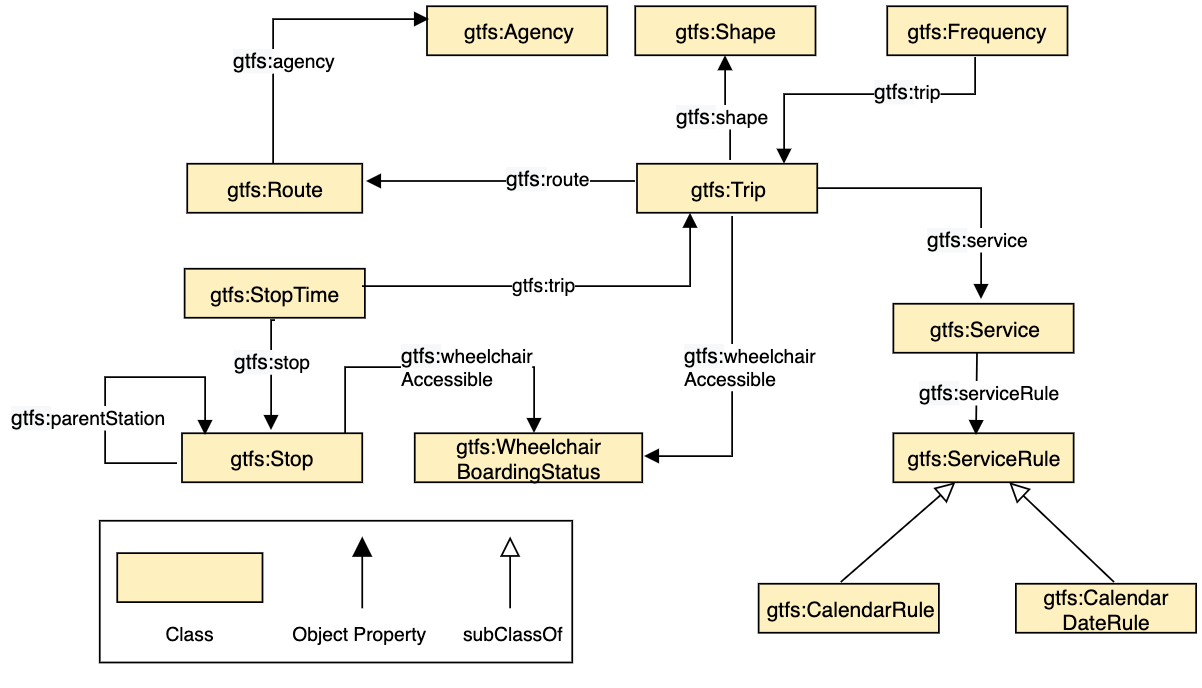
\includegraphics[width=0.8\linewidth]{figures/GTFSontology.png}
    \caption[The LinkedGTFS Ontology]{\textbf{LinkedGTFS Ontology.} Subset of the LinkedGTFS ontology used in the GTFS-Madrid-Bench for virtual knowledge graph access. There are eleven object property relations among the classes, and two subClassOf relations.}
    \label{fig:gtfsOntology}
\end{figure}

\subsubsection{Dataset Generation}

Dataset generation for a virtual knowledge graph access benchmark should be focused on the two main variables that allow testing the capabilities of the engines: (i) data size, and (ii) formats in which data can be expressed. In the context of data generation for OBDA, VIG~\citep{lantivig} proposes the use of R2RML mappings for an efficient scale up of the size of an instance of an RDB dataset. In this case, only one data format (SQL) is involved in the process. 

We use GTFS as the original data source for several reasons: First, GTFS has been the \textit{de-facto} standard for publishing transport data on the web, it also comes with a clear specification, making it easy to understand. Second, the GTFS model comprises several entities that are related through a variety of relationships. In addition it includes different data types such as strings, integers, and booleans. Finally, many cities have adopted the GTFS data model and have published their GTFS data online. Although in our benchmark we propose the use of the GTFS Madrid subway data, GTFS data from a different city could be used as the original data source.

The GTFS-Madrid-Bench proposes an extended workflow using VIG as the Dataset Generator engine for the generation of the datasets taking into account multiple data formats (see an example in Figure \ref{fig:generation}). We describe the detailed steps of the proposed data generation workflow together with examples following the definitions provided in Section \ref{sec:preliminars}:

\begin{enumerate}[label=\textbf{\arabic*})]
    \item \textbf{Data preparation.} The original data source, GTFS, is in CSV format. VIG requires an instance of an RDB and an R2RML mapping for scaling up the data source. We use Morph-CSV\footnote{\url{https://github.com/oeg-upm/morph-csv}}, which takes as inputs a set of spreadsheets in the form of CSV files, their corresponding annotations using CSVW~\citep{tennison2015model} and an RML mapping~\citep{dimou2014rml}. It automatically produces the corresponding schema of an RDB (identifying typical constraints such as datatypes, PK/FK, indexes and NULLs) and an R2RML mapping document, which are the inputs for VIG. 
    
    For the Madrid-GTFS-Bench, we use as input an open data dataset GTFS$_{mad}^{CSV}$ = (GTFS$_{mad}$, GTFS, CSV). GTFS$_{mad}$ is the set of data sources of the subway network of Madrid that has been provided by its transport authority according to the schema GTFS as described in its specification\footnote{\url{https://developers.google.com/transit/gtfs/}}. This dataset is composed of a set of CSV files containing data of Agency, Route, Shape, Frequency, Trip, StopTime, Stop, Calendar and CalendarRule. This input is fixed during all of the data generation process, which means that the generated datasets are defined by the same schema and all of the generated data is obtained from this initial dataset. We create the corresponding RML mapping rules and CSVW metadata annotations and, using the Morph-CSV engine, we generate the corresponding RDB instance GTFS-SQL-1=(GTFS$_{mad}^{SQL}$,1) dataset and the R2RML mapping rules.
    
    \item \textbf{Data creation.} VIG~\citep{lantivig} takes into account the ontology and the set of R2RML mappings to generate each dataset. This engine also receives as input a scale value $s$ that indicates that the size of each table of the database increases $s$ times. The output of VIG is a set of CSV files, one file for each table of the RDB. In this step the dataset GTFS-CSV-s=(GTFS$_{mad}^{CSV}$,s) is generated, where $s$ is the selected scale value.
    
    \item \textbf{Data distribution.} Finally, each dataset generated using VIG is distributed in several formats. We use open source tools to perform this step such as csv2json, from Python CSVKit\footnote{\url{https://csvkit.readthedocs.io/en/1.0.3/scripts/csvjson.html}} and di-csv2xml\footnote{\url{https://github.com/blue-yonder/di-csv2xml}}, depending on the data formats (JSON and XML). We divide the distribution into two categories in order to cover both OBDA and OBDI approaches: 
    
    In the first category, focused on providing support to OBDA techniques, the sources of each dataset are transformed into a single format (e.g., CSV files are transformed into JSON files). The datasets are transformed to the corresponding ones in JSON, XML, SQL and MongoDB obtaining the following datasets: GTFS-F-s$=$(GTFS$_{mad}^{F}$,s) where $s$ is the scale value and F $\in$ $\{$JSON, XML, SQL, MongoDB$\}$. 
    
    In the second category, focused on virtual KGC approaches, the sources of each dataset have to be transformed from the CSV files into multiple formats (e.g. CALENDAR is a JSON document, AGENCY is a XML file, etc.). To distribute the files and based on the GTFS model, the user may select the sources associated to each format and then the benchmark generates the dataset and the corresponding set of mapping rules. 
    
    Additionally, the benchmark provides by default two datasets taking into account the selected formats (JSON, CSV, XML, SQL and MongoDB) where the number of relations (joins) among sources in different formats is minimized or maximized. The formats of the sources in these datasets is also configurable during the generation data process, in order to allow users to analyze the impact of joins over formats with different features. For example, the join selectivity between shapes and trips is different than the join selectivity between routes and agencies, and depending on the formats of each source, the total query execution time of a processor may be impacted. We describe each dataset in more detail:
    \begin{itemize}
        \item Best Dataset: The number of joins among sources in different formats is minimised but ensuring that all of the formats are covered. The aim of this configuration is to study the behavior of the engines when they have to deal with different data sources but where most of the joins are done between sources in the same format. Hence they may delegate their treatment to the underlying data source manager (e.g. MySQL in RDB) and apply common optimisation techniques in query translation approaches~\citep{priyatna2014formalisation}. To meet this requirement and, having 5 possible formats for the data sources, the proposed groups for best dataset are: trips, shapes, calendar and calendar\_dates sources in one group, routes and agency in another, frequencies in the third group, stop and stop\_times in the fourth one and feed\_info in the last one. This composition generates the GTFS$_{mad}^{B}$ dataset. We show a possible example of a best dataset in Figure \ref{fig:best}. 
       
        \item Worst Dataset: The number of joins among sources in different formats is maximised and the five formats are covered. In this distribution, all the possible joins are among sources in different formats. This means that the virtual KGC engine may be enforced to perform the joins after the execution of the translated queries over the original data sources. In the same manner as the best dataset, the groups of sources are: shapes and stops in one group, trips and feed\_info in another, calendar and agency in the third group, routes and stop\_times in the fourth and calendar\_dates and frequencies in the last one. This composition generates the GTFS$_{mad}^{W}$ dataset. We show a possible example of the worst dataset in Figure \ref{fig:worst}. 
    \end{itemize}
   
\end{enumerate}
 

\begin{figure}[h]
    \centering
    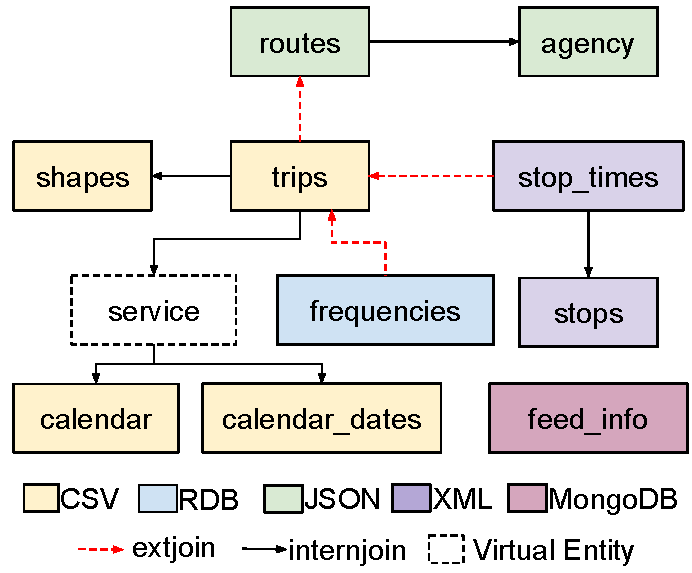
\includegraphics[width=0.85\linewidth]{figures/best-dist.pdf}
    \caption[Example of best dataset]{\textbf{Example of Best Dataset}. Best dataset distributes the formats over the data sources ensuring that at least there is one source per each format and the joins among different formats are minimised. \textit{extjoin} means that there is a relation between sources in different formats and \textit{internjoin} means that the joins are between sources in the same format.}
    \label{fig:best}
\end{figure}


\begin{figure}[h]
    \centering
    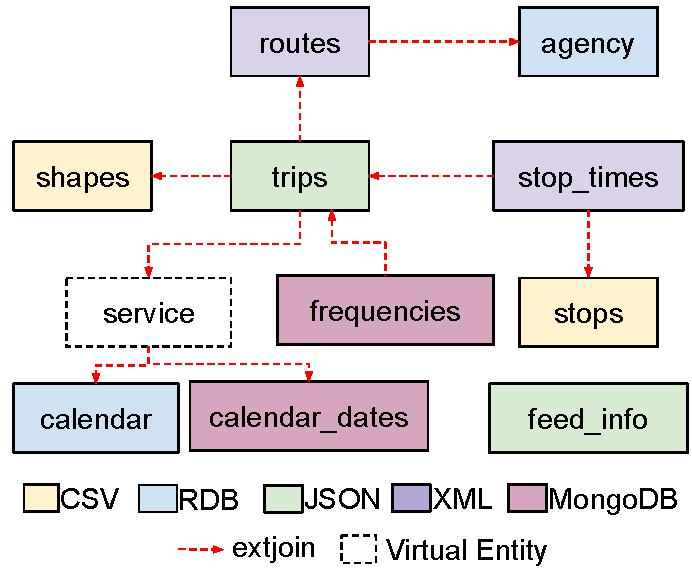
\includegraphics[width=0.85\linewidth]{figures/worst-dist.pdf}
    \caption[Example of worst dataset]{\textbf{Example of Worst Dataset}. Worst dataset distributes the formats over the data sources ensuring that at least there is one source per each format and the joins among different formats are maximised. \textit{extjoin} means that there is a relation between sources in different formats.}
    \label{fig:worst}
\end{figure}

\begin{figure}
    \centering
    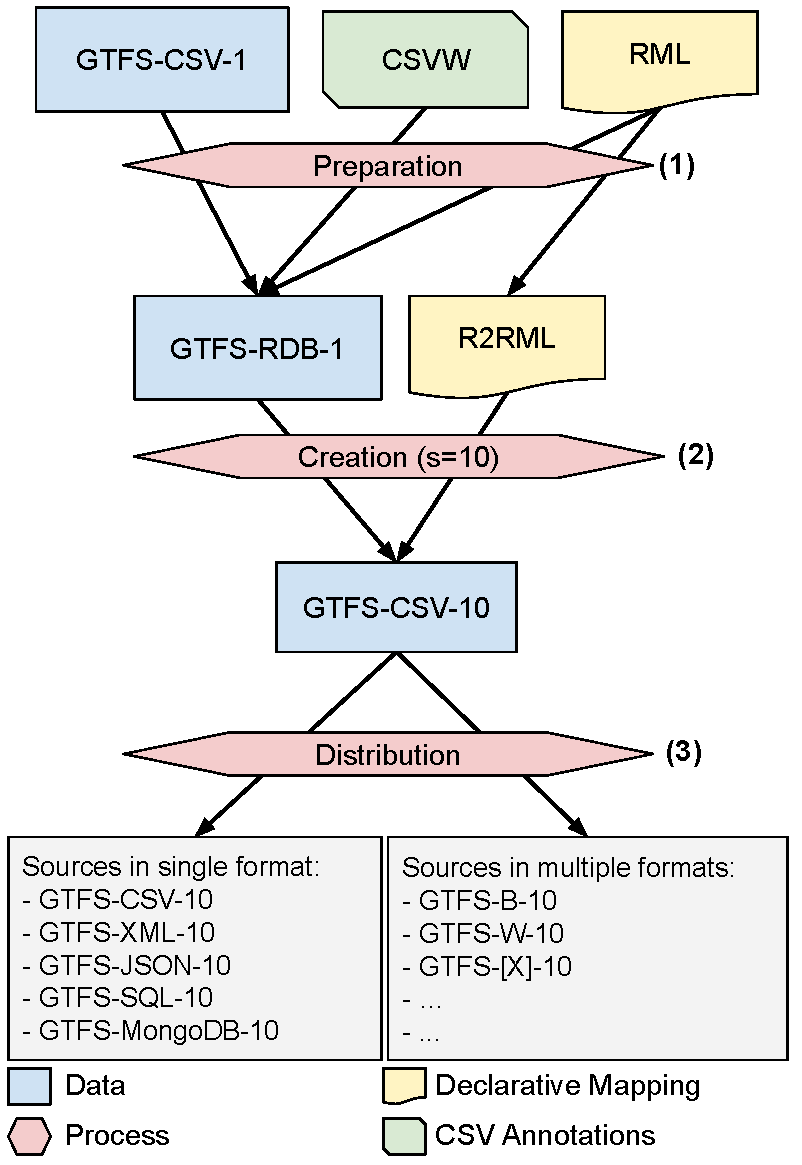
\includegraphics[width=0.7\linewidth]{figures/gprocess.pdf}
    \caption[Generation workflow for scale value 10]{\textbf{GTFS-Madrid-Bench Generation Workflow with scale value 10}. From the original 10 CSV files of Madrid Metro GTFS we use (i) Morph-CSV to generate the corresponding RDB instance and an R2RML mapping that are the required inputs for (ii) scaling up the data using VIG and (iii) distributing the generated CSV dataset to the different formats.}
    \label{fig:generation}
\end{figure}

We want to be able to compare the results obtained by processors with the results obtained by the materialized graph in RDF. For this purpose, we take the output of VIG (e.g., GTFS-CSV-5, GTFS-CSV-10) and we run a materialized KGC process using the SDM-RDFizer\footnote{\url{https://github.com/SDM-TIB/SDM-RDFizer}} engine, which generates the KG in RDF using RML mapping rules. We select this tool because it passed all the RML Test Cases~\citep{heyvaert2019conformance} for CSV files\footnote{\url{http://rml.io/implementation-report/}}, hence we assume that the generation is correct, and that it provides a set of techniques to optimize the generation of RDF at scale. 

\begin{table}[]
\centering
\caption[Mapping features of GTFS]{\textbf{Mapping features of GTFS.} Each TriplesMap of the GTFS mapping file and its corresponding features: the related source, number of Classes, PredicateObjectMaps, Predicates, Objects and RefObjectMaps (joins). }
\label{tab:mappings}
\resizebox{0.9\textwidth}{!}{%
\begin{tabular}{l|l|l|c|c|c|c}
\hline
\multicolumn{1}{c|}{\textbf{TriplesMap}} & \multicolumn{1}{c|} {\textbf{Source}} & {\textbf{Classes}} & \textbf{\#PredicateObjectMap} & \textbf{\#Predicates} & \textbf{\#Objects} & \textbf{\#RefObjectMap} \\ \hline
shapes          &  shapes              & gtfs:Shape                               & 4                     & 4            & 4         & 0      \\ \hline
trips           &  trips              & gtfs:Trip                               & 8                     & 8            & 5         & 4      \\ \hline
calendar\_rules         & calendar              & gtfs:CalendarRule                               & 9                     & 9            & 9         & 0      \\ \hline
calendar\_date\_rules   &  calendar\_dates            & gtfs:CalendarDateRule                               & 2                     & 2            & 2         & 0      \\ \hline
stops              &    stops         & gtfs:Stop                               & 12                    & 12           & 11        & 1      \\ \hline
stoptimes         & stop\_times           & gtfs:StopTime                               & 9                     & 9           & 7         & 2      \\ \hline
routes               &  routes         & gtfs:Route                               & 8                     & 8            & 7         & 1      \\ \hline
agency                & agency          & gtfs:Agency                               & 6                     & 6            & 6         & 0      \\ \hline
frequencies       &  frequencies              & gtfs:Frequency                               & 5                     & 5            & 4         & 1      \\ \hline
feed      &  feed\_info               & gtfs:Feed                               & 6                     & 6            & 6         & 0      \\ \hline
service1 &   calendar           & gtfs:Service                               & 1                     & 1            & 0         & 1      \\ \hline
service2 & calendar\_dates       & gtfs:Service                               & 1                     & 1            & 0         & 1      \\ \hline
\textbf{Total}      &  \multicolumn{1}{c|}{10}    & \multicolumn{1}{c|}{11}                           & 71                     & 71            & 60         & 11      \\ \hline
\end{tabular}%
}

\end{table}

\subsubsection{Mappings} 
Mappings play one of the most important roles in the benchmark since they are the main element used for the query translation process. In the state of the art there are multiple engines and tools that use different mapping languages. We select a set of the most relevant declarative mapping languages in the state of the art and we generate the corresponding mapping rules. In more detail, the GTFS-Madrid-Bench provides:
\begin{itemize}
    \item One R2RML mapping document for accessing SQL datasets.
    \item One xR2RML mapping document for accessing MongoDB datasets.
    \item Seven RML mapping documents\footnote{Provided in RML and YARRRML serializations} for accessing CSV, JSON, XML, SQL, MongoDB, Best and Worst datasets.
    \item One CSVW metadata file to provide annotations for the CSV datasets.
\end{itemize}
Conceptually, all the mappings represent the same relations among the concepts of the ontology and the concepts of the GTFS model, but each one has been developed according to a specification that handles the characteristics of each data format. The mappings are composed by a set of rules representing the relation of one element in the ontology with the corresponding schema element from a source. An overview of the rules within the mappings developed for this benchmark is shown in Table \ref{tab:mappings}. The rules of the mappings are very relevant since they contain many parameters that impact on the performance of the virtual knowledge graph access engines~\citep{chaves2019what}. 

More in detail, each source of the GTFS feed has one associated TriplesMap with a rule to associate the generated entities to the class defined in the ontology, and a set of rules for the object and data properties. Additionally, there is a (virtual) entity, Service, in the data model with no corresponding source, what implies the definition of a set of mapping rules to generate the instances of the corresponding class (\texttt{gtfs:Service}). Following the GTFS specification, the identifier of Service can be found either in calendar or calendar\_dates sources. This means that to be aligned with standard declarative mapping specifications (e.g. RML and R2RML only allow one source per TriplesMap), the mapping document needs to define two TriplesMap, one for calendar (service1) and another for calendar\_dates (service2). This also implies that the trips TriplesMap has one predicate (\texttt{gtfs:service}) with two associated refObjectMaps, where the parentTriplesMap are service1 and service2; this allows generating all \texttt{gtfs:Service} defined in the original data source. Because the instances of \texttt{gtfs:WheelchairBoardingStatus} class are only objects in \texttt{gtfs:Trips} and \texttt{gtfs:Stops} triples, they are generated using the template property in trips and stops TriplesMap. In summary, the mapping contains rules to generate instances of 12 classes, 71 PredicateObjectMaps and Predicates, 60 Objects and 11 RefObjectMaps, covering the main features defined in state-of-the-art mapping specifications for KGC. All of the GTFS mappings are detailed in Appendix \ref{sec:appendix2} using the YARRRML~\citep{Heyvaert2018Declarative} serialisation.

% Queries
\subsubsection{Queries}
Table \ref{tab:queries} presents all the variables considered for the 18 queries in our benchmark. We have developed queries that are based on the Linked GTFS ontology, and are aligned with user stories in Madrid's transport domain, together with different combinations of values for the variables. It should be mentioned that the queries cover all of the data sources that were generated by the Madrid's transport authority as GTFS data from the metro system. These include agencies, routes, stops, trips, frequencies, shapes, calendar, and calendar dates. Although in the benchmark we have defined mappings to translate queries into the underlying query language of the source, these are independent from the queries (we have used these mappings to generate the materialized knowledge graph in the data generation step).

We have defined two sets of 18 queries with identical templates but differences in the constants that appear in subjects or objects of bounded triple patterns: (1) Baseline queries with constants that belong to Madrid's GTFS Linked Data, and (2) VIG queries with constants that belong to the datasets generated by the tool; these queries are executed in the evaluation described in Section \ref{sec:evaluation}. 

\begin{sidewaystable*}[p]
\centering
\caption{GTFS-Madrid-Bench Queries}
\label{tab:queries}
\resizebox{1\textwidth}{!}{%
\begin{tabular}{c|l|c|c|c|c|c|c|c|c|c}
\hline
%Query & Description & \#Triple  & \#Sources & OPTIONAL & Aggregation & Other & FILTER & FILTER & Star-shaped groups  \\ 
Query & Description & \#Triple  & \#Sources & OPTIONAL & Aggregation & Other & \multicolumn{2}{ |c| }{FILTER} & \multicolumn{2}{ |c }{\#Star-shaped groups} \\   
 &  & Patterns  &  & &  & features  & equal to & relational  &  w/o constants & w/constants \\ \hline
q1 & All shapes & 4 & 1 &  &  &  &  &  & 1 & 0 \\ \hline
q2 & All stops where the latitude is larger than a & 5 & 1 & \checkmark &  &  &  & \checkmark & 0 & 1 \\ 
&  specific value &  &  &  &  &  &   &   &  & \\ \hline
q3 & Accessibility information of all stations & 5 & 1 & \checkmark &  &  & \checkmark &  & 0  & 1 \\ \hline
q4 & All agencies and their routes & 9 & 2 & \checkmark &  &  &  &  & 2 & 0 \\ \hline
q5 & Services that have been added after a specific date& 5 & 2 &  &  &  &  & \checkmark & 1 & 1 \\ \hline
%&  specific date  &  &  &  &  &  &   &   &  & \\ \hline
q6 & Number of routes covered by a specific agency & 3 & 2 &  & \checkmark &  & \checkmark &  &  0  & 2 \\ \hline
q7 &  All wheelchair-accessible stops in a specific route   & 15 & 4 & \checkmark &  & DISTINCT & \checkmark &  & 1 & 3 \\ \hline
q8 & Routes and their related trips, services, stops and stop times & 14 & 5 & \checkmark &  &  &  &  & 5 & 0 \\ \hline
q9 &  Trips and associated shapes where latitude  & 7 & 2 & \checkmark &  &  &  & \checkmark & 1 & 1 \\ 
 &  is larger than a specific value &  & &   &  &  &   &  &   &   \\ \hline
q10 &  Number of trips that have a duration   & 4 & 2 &  & \checkmark & DISTINCT &  & \checkmark & 1 & 1 \\ 
 &  over a number of minutes &  &  &  &  &  &   &   &  & \\ \hline
q11 & Trips that are available on a certain date  & 12 & 3 &   &  & NOT EXISTS &  & \checkmark & 3 & 2 \\ \hline
 %&  &  &  &   &  &  &  &  &  & \\ \hline
q12 & Number of stops that are wheelchair-accessible  & 10 & 4 &   & \checkmark & GROUP BY &  &  & 3 & 1 \\ 
 & grouped by route  &  &  &   &  &  &  &  &  & \\ \hline 
q13 & The accesses of all stations & 6 & 1 &  \checkmark &  &  &  &  & 0 & 1 \\ \hline
q14 & All stops times and their related routes and stops ordered by  & 8 & 3  & \checkmark &  & ORDER BY &  &  & 3 & 0 \\ 
  & their sequence, in a specific direction and service  &  &   & &  &  &  &  & & \\ \hline
q15 & For all properties, triples that contain  & 3 & 1 &    &  &  & \checkmark &  & 0 & 1 \\ 
 &  a specific  word in the object placeholder  &  &  &    &  &  &  &  & & \\ \hline
q16 & For all routes, all calendar changes in  & 8 & 3 &    &  &  &  & \checkmark & 2 & 1 \\ 
 &  a specific month &  &  &    &  &  &  &  & & \\ \hline
q17 & Trips with their start and end time  & 9 & 3 &   &  &  &  &  & 3 & 0 \\  
 & of the frequencies and associated routes    &  & &   &  &  &  &  & & \\  \hline
q18 & All routes that have trips on Sunday  & 8 & 5 &   &  & UNION &  &  & 4 & 1 \\ \hline 
\end{tabular}%
}
\end{sidewaystable*}


\subsubsection{Metrics}
In this section we define the metrics that are used to evaluate the performance of Virtual Knowledge Graph access engines. The metrics consider the workflow followed by Virtual Knowledge Graph systems, and for each of the steps identified in the workflow we introduce a set of metrics to be measured and reported.
\begin{table}[]
\caption[Metrics VS dimensions]{Relation between each relevant metric for the Madrid-GTFS-Bench and the dimensions that can impact over that metric. In the Dimension column, Q means query, M mappings and D data.}
\label{tab:dimsensions}
\begin{tabular}{l|c|c}
\hline
\multicolumn{1}{c|}{\textbf{Metric}} & \textbf{Type or Phase} & \textbf{Dimension}  \\ \hline
\multicolumn{3}{c}{General Metrics}                                                 \\ \hline
Total execution time                & General                & D, Q, M \\ \hline
\# answers                            & General                & D, Q, M \\ \hline
Initial delay                         & General                & D, Q, M \\ \hline
Dief@k                                & C. Behaviour           & D, Q, M \\ \hline
Dief@t                                & C. Behaviour           & D, Q, M \\ \hline
\multicolumn{3}{c}{Specific Metrics (Phases)}                                       \\ \hline
Loading time                          & Starting        & Q, M      \\ \hline
Mapping trans. time              & Starting         & M              \\ \hline
\# requests                           & Distribution      & Q              \\ \hline
Source selec. time                 & Distribution      & Q, M     \\ \hline
Query gen. time                 & Distribution      & Q               \\ \hline
Query rewrit. time                  & Rewriting     & Q                \\ \hline
Query trans. time                & Translation    & Q, M       \\ \hline
Query exec. time                  & Execution     & Q, D          \\ \hline
Query aggreg. time                & Finishing         & D                 \\ \hline
\end{tabular}
\end{table}

The workflow extends the OBDA phases identified by Mora and Corcho~\citep{mora2013towards}, and Lanti et al.~\citep{lanti2015npd}. In addition, it includes some of the steps that are defined by proposals that federate queries~\citep{schwarte2011fedx}. General metrics to be captured are \textbf{overall execution time}, \textbf{completeness of answers} and \textbf{initial delay}. Other metrics may be considered when the engine generates answers following a continuous behavior~\citep{sharaf2008algorithms}, such as \textbf{dief@k} or \textbf{dief@t} proposed in \citep{acosta2017diefficiency}. Additionally, for each phase of a workflow, a virtual knowledge graph construction engine may capture specific metrics that allow the identification of bottlenecks in the implementations. This relevant set of metrics for each phase are: (i) \textbf{loading time} during the starting phase when the ontology, mappings and query are loaded; (ii) \textbf{total number of requests} and \textbf{source selection time} during the source selection phase (the engine identifies the sources that can be used to answer the query); (iii) \textbf{query generation time} when the set of sub-queries to be evaluated over each data source is created, and the query plan is generated; (iv) \textbf{mapping translation time} when the engine requires to translate a provided mapping into another one in in a different language, maintaining a set of properties between them~\citep{corcho2019towards}; (v) \textbf{query rewriting time} when the generated sub-queries are rewritten to other queries, taking into account potential inferences from the ontology and information in the mapping~\citep{mora2014kyrie2}; (vi) \textbf{query translation time} when the engine, taking the mapping into account, translates each sub-query to another one in the query language supported by the underlying data sources such as SPARQL-to-SQL~\citep{chebotko2009semantics}; (vii) \textbf{query execution time} when the translated queries are evaluated against the underlying data sources and the results are translated to RDF or as SPARQL bindings using the rules provided in the mappings; and (viii) \textbf{query aggregation time} when the results obtained for each sub-query are aggregated, including the removal of duplicates and the linking of resources. Variables that have an impact on the metrics have been grouped into three dimensions: Query, Data, and Mappings. The relation between each  metric considered  and the dimensions that can impact over that metric is  shown in Table \ref{tab:dimsensions}.

\noindent\paragraph{\textbf{Query.}} The Query dimension variables refer to the structure of the queries, e.g. \#triple patterns, \#sources, and  \#star-shaped groups. A  Star-shaped group is a group of triple patterns that are ``joined" over the same subject or object variable~\citep{vidal2010efficient}. The most common case in real-world scenarios are subject star-shaped groups that represent properties that describe one source. The benchmark considers an increasing number of triple patterns, from 3 to 15, also the number of sources vary from 1 to 5. In particular we have several queries on 1 source with a varying number of triple patterns, and queries that have a large number of triple patterns combined with 4 and 5 sources. With respect to these two variables, our aim is to balance real-life use cases where several properties in the specification need to be combined and retrieved, and query complexity (worst case scenario is the ``Worst Dataset'' when the five sources are represented in the five available formats and the number of joins among sources is maximized).Furthermore, a large number of sources or triple patterns  combined with a large number of non-instantiated star-shaped groups should impact overall execution time and also specifically impact query generation, query rewriting, query translation, and query execution times. 

In general, queries in GTFS-Bench-Madrid combine those that contain single star-shaped groups ($q1$,$q2$, $q3$, $q15$) with those that contain chains of star-shaped groups, that is, where the object of a pattern in a group is the subject in the next group (with joins across different sources): $q4$, $q5$, $q6$, $q7$, $q9$, $q10$, $q11$, $q12$, $q16$, $q17$, $q18$. According to the ontology structure shown in Figure \ref{fig:gtfsOntology}, \texttt{gtfs:StopTime} relates to stops and trips and may lead to hybrid shapes such as $q8$ and $q14$. There is also the case of query $q13$, which refers one source and contains a self-join that relates an access to a station to its ``parent'' station.

Besides, as mentioned in~\citep{montoya2012benchmarking}, query plans generated by query evaluation systems during the subquery generation phase may be affected by the structural properties of a query. If the sources in the dataset are all represented in the same format, then query plans will be generated by the underlying engine (either an RDB engine or a NoSQL engine), and execution time will be affected by the number of joins within star-shaped groups and among these groups. When the sources of the dataset are not in the same format, the engine has to create the query plan. The performance will be affected by the plan proposed by the engine. Different combinations of these variables are considered in GTFS-Madrid-Bench queries: on the one hand we have a large number of triple patterns, sources and star-shaped groups in $q7$ and $q8$, and on the other hand queries like $q18$ combine a large number of sources and star-shaped groups with a medium-sized query (8 triple patterns).

Complexity of SPARQL queries is presented in~\citep{perez2009semantics}, considering the SPARQL fragment with only AND and FILTER operators. Complexity is linear on the product of the dataset size and the size of the query (\# triple patterns), and evaluation is NP-complete for queries constructed with AND, FILTER and UNION operators. Several queries in GTFS-Madrid-Bench have FILTER clauses and specifically, $q18$ contains a UNION of two triple patterns.

The evaluation problem becomes harder when the OPTIONAL operator is added~\citep{perez2009semantics}. Additionally, the work described in~\citep{xiao2018efficient} presents optimization techniques applied in an OBDA setting specifically for queries that have to deal with OPTIONAL triple patterns, claiming that the underlying database systems do not optimize adequately these class of queries. Similar problems may be expected for querying CSV, XML and JSON data sources. We have designed eight queries that use OPTIONAL graph patterns (according to the corresponding non-mandatory attributes in the specification). 

Constants in triple patterns together with FILTER with equality operators increase the selectivity of queries and are likely to reduce the cost of evaluating the query. According to~\citep{montoya2012benchmarking}, instantiated triple patterns have an important impact on the potential number of join intermediate results that may be generated throughout query execution. However, using a FILTER relational operator specially in the case of open ranges, e.g. a FILTER with a $>$ operator, may generate a large number of answers. We have considered several combinations of number of star-shaped groups with and without constants, $q8$ has no constants whereas in $q4$ both star-shaped groups in the query have bindings. An example of an intermediate case occurs in $q12$ with 1 out of 4 instantiated star-shaped groups. 

Three queries contain the aggregated COUNT function, and one of these queries contains additionally the GROUP BY modifier. Other queries use language features like DISTINCT and ORDER, what will impact on the query execution time metric because all of them require an ordering of the tuples/entries of the underlying sources. We cover the impact of these variables in $q7$ and $q10$ with DISTINCT, and $q12$ and $q14$ with GROUP BY and ORDER BY respectively. Finally, having unbounded predicates in a query ($q15$) increases its complexity because the search space during query evaluation may be large. 

The work in~\citep{angles2016negation} studies the impact of negation in the computational complexity of SPARQL queries, it distinguishes four types of negation: negation of filter constraints, negation as failure, negation by MINUS and negation by NOT EXISTS.  The use of NOT EXISTS introduces similar issues to sub-query evaluation because of the  presence of correlated variables and the use of a nested iteration method to evaluate queries that contain this type of negation. Hence $q11$ contains negation with NOT EXISTS.


\noindent\paragraph{\textbf{Mappings.}}
Features of mappings are relevant because they may impact  the performance of the engines. Previous work by~\citep{chaves2019what} evaluates different mapping variables that impact in the construction of a knowledge graph. Similarly, we consider that the following mapping variables influence overall query execution time and specifically query translation and query rewriting times. Regarding structure, we have considered the variables \#Classes, \#PredicateObjectMaps, \#Predicates, \#Objects, and \#RefObjectMap that are presented in Table \ref{tab:mappings}. Another variable is relation type, the mappings of the Madrid-GTFS-Bench include 1-1, 1-N, N-1 and N-M relation types. In general mappings for sources that represent N-M relationships (e.g. stop\_times) are more complex and thus time consuming for query execution. Additionally, the variable \texttt{rr:termtype} of the \texttt{rr:objectMap} may also have an effect because the cost of generating a constant, a reference or a template is not the same.

\noindent\paragraph{\textbf{Dataset.}}
Variables in this dimension include dataset size and the formats of its sources. As already mentioned in Section \ref{sec:datageneration}, datasets with different scale factors are generated in GTFS-Madrid-Bench. Size has an impact on the overall execution time, on the initial delay, and specifically on query execution time because of the larger number of intermediate results. It also influences query aggregation time because in the benchmark, queries against larger datasets generate a larger number of answers.

The format variable may take a single value for datasets in only one format (RDB, CSV, XML, MongoDB, JSON) or multiple formats (Best, Worst and Random). This variable has an impact on the overall execution time, specifically on the query translation and query execution times, as well as on the number of answers because  different formats have different access methods and different underlying query languages.

The work in~\citep{montoya2012benchmarking} presents partitioning and data distribution in this dimension. In GTFS-Bench-Madrid there are fixed values for these variables: the partitioning is vertical and datasets and databases are loaded in local machines.

\subsection{Sustainability and extensibility}
The Madrid-GTFS-Bench is supported by a set of robust resources in order to ensure its sustainability. The benchmark can be adapted to any other virtual knowledge graph access engine that uses other mapping rules languages, or to other non-declarative proposals. The developers or users only have to create the mapping documents according to that specification. Additionally, virtual knowledge graph access engines that work with other graph query languages (e.g. Morph-GraphQL~\citep{priyatna2019morph}) can take advantage of our proposed benchmark. 

A set of improvements for the data generation that we have identified are based on VIG, a robust and efficient engine for the generation of scalable datasets. Additionally, all the generated resources are available online \footnote{\url{https://github.com/oeg-upm/gtfs-bench/}} and their deployment (engines and databases) is done using docker images to ensure the reproducibility of the obtained results. Finally, because we define the dimensions of mappings and datasets taking into account the relevant parameters in the process of constructing knowledge graphs~\citep{chaves2019what}, this benchmark can be also used to test the materialization KGC engines such as RMLMapper~\footnote{\url{https://github.com/RMLio/rmlmapper-java}}, RocketRML~\footnote{\url{https://github.com/semantifyit/RocketRML/}} or SDM-RDFizer~\footnote{\url{https://github.com/SDM-TIB/SDM-RDFizer}} since, at this moment, there is no proposal to evaluate the performance and completeness of these engines in an objective manner.

The possibility to extend this benchmark is also one of the main points that differentiates this proposal to previous ones. First, there are multiple benefits obtained from relying on an open data model from the transport domain, such as linking this data with other data from the city and also having other GTFS transport systems feeds (e.g. metro and train datasets). In addition to queries that take into account the specific characteristics of the selected datasets, it is also possible to incorporate more complex mapping rules with extended features such as specific transformation functions~\citep{de2016ontology}, something that is difficult to address by previous proposals as their data model is usually relational database oriented ~\citep{bizer2009berlin,lanti2015npd}. The incorporation of these features will ensure that we cover new characteristics of the new generation of virtual knowledge graph access engines without the need of creating a benchmark from scratch.  


\subsection{Experimental Evaluation}
In this section we describe the evaluation performed using our benchmark. We first describe the selected virtual KGC engines involved in the evaluation, we describe the evaluation methodology and infrastructure, based on the use of docker images to ensure the reproducibility of the experiments, and finally, we provide the obtained results. All the resources used in this evaluation, such as queries, data, mappings, running scripts, results and docker images for engines and databases are publicly available online\footnote{\url{https://github.com/oeg-upm/gtfs-bench}}.

\subsubsection{Tools}

We selected the most relevant open source virutal KGC engines in the state of the art: 

\noindent\textbf{Ontario.} Ontario~\citep{endris2019ontario}\footnote{\url{https://github.com/SDM-TIB/Ontario}} is an virtual KGC engine from heterogeneous data sources that is based on the concept of RDF molecule templates (RDF-MT)~\citep{endris2017mulder}. Ontario exploits the information provided by the mapping rules for creating the corresponding RDF-MT over the data sources. After the source selection and sub-query generation processes, Ontario translates the SPARQL query into the corresponding query language of the original data source. It supports the following formats: RDF, MySQL, CSV, TSV, JSON, XML, MongoDB and Neo4j.

\noindent\textbf{Ontop.} Ontop~\citep{rodriguez2015efficient}\footnote{\url{https://github.com/ontop/ontop}} is an KGC system from RDB instances that includes both materialization and virtualization techniques. Ontop translates R2RML mappings into its own mapping language, called ``OBDA mappings''. These mappings, and a SPARQL query if available, are transformed into datalog rules, allowing semantic optimization techniques to be applied, and generating efficient SQL queries (e.g., self-join elimination). It only supports the SQL format.

\noindent\textbf{Morph-RDB.} Morph-RDB~\citep{priyatna2014formalisation}\footnote{\url{https://github.com/oeg-upm/morph-rdb}} is an R2RML engine that also includes materialization and virtualization techniques. The formalization of its query translation technique is based on the R2RML-based extension of SPARQL-to-SQL query translation algorithm proposed by~\citep{chebotko2009semantics}, originally designed to work with RDB-backed triples store. Similar to Ontop, several optimization techniques are also incorporated in order to generate more efficient SQL queries. It supports SQL and CSV files.

\noindent\textbf{Morph-xR2RML.} Morph-xR2RML~\citep{michel2015translation}\footnote{\url{https://github.com/frmichel/morph-xr2rml}} uses the xR2RML mapping language to support the generation of RDF lists, and to query data stored in NoSQL databases such as MongoDB.

\noindent\textbf{Morph-CSV.} Morph-CSV~\citep{chaves2020enhancing}\footnote{\url{https://github.com/oeg-upm/morph-csv-sparql}} exploits the information of CSVW annotations and RML mappings to enforce implicit constraints over tabular data, explicitly declared in these annotations. It can be integrated on top of any existing SPARQL-to-SQL engine in order to enhance query completeness and performance.

We also intended to include other engines such as Squerall~\citep{mami2019querying} or Polyweb~\citep{khan2019one}. In both cases, either the code is not available as open source or it was not feasible to run the engine due to the lack of documentation. Issues have been reported in their corresponding repositories, with the intention of alerting the authors and maintainers about the current limitations.

\subsubsection{Setup}
In this section we describe how we use our benchmark to evaluate several processors/engines that have been described in Section \ref{sec:tools}. 

We have setup several experiment configurations for evaluating the selected processors. As an example, the experiment configurations for query $q4$ can be seen in Table \ref{tab:ExperimentalEnvironment}. These experiment configurations have a fixed set of mappings with routes and agencies. The processor used to evaluate this query depends on the dataset, for example, Ontario in the case of the JSON dataset or Morph-RDB, Ontario and Ontop for SQL.

\begin{table}[]
\centering
\caption[Experiment configuration example set]{\textbf{Experiment configuration example set.} List of experimental configurations and processors for q4. $D$ is a dataset where $s$ is the scaling factor (i.e., 1, 5, 10, 50, 100, 500), $M$ is the set of mappings, $q$ is the SPARQL query, $\phi$ is a processor. $q$ is a SPARQL query defined in the Appendix Section.}
\label{tab:ExperimentalEnvironment}
\resizebox{0.8\textwidth}{!}{%
\begin{tabular}{c|c|c|c}
\hline
\textbf{Query $q$} & \textbf{Dataset $D$} & \textbf{TriplesMap $M$} & \textbf{Processor $\phi$} \\ \hline
\multirow{11}{*}{q4} & \multirow{3}{*}{GTFS$_{mad}$-CSV-s} & \{routes,agency\}$_{RML}$ & Morph-CSV \\ \cline{3-4} 
 &  & \{routes,agency\}$_{R2RML}$ & Morph-RDB \\ \cline{3-4} 
 &  & \{routes,agency\}$_{RML}$ & Ontario \\ \cline{2-4} 
 & \multirow{3}{*}{GTFS$_{mad}$-SQL-s} & \{routes,agency\}$_{R2RML}$ & Morph-RDB \\ \cline{3-4} 
 &  & \{routes,agency\}$_{RML}$ & Ontario \\ \cline{3-4} 
 &  & \{routes,agency\}$_{OBDA}$ & Ontop \\ \cline{2-4} 
 & GTFS$_{mad}$-MongoDB-s & \{routes,agency\}$_{xR2RML}$ & Morph-xR2RML \\ \cline{2-4} 
 & GTFS$_{mad}$-XML-s-s & \{routes,agency\}$_{RML}$ & Ontario \\ \cline{2-4} 
 & GTFS$_{mad}$-JSON-s & \{routes,agency\}$_{RML}$ & Ontario \\ \cline{2-4} 
 & GTFS$_{mad}$-B-s & \{routes,agency\}$_{RML}$ & Ontario \\ \cline{2-4} 
 & GTFS$_{mad}$-W-s & \{routes,agency\}$_{RML}$ & Ontario \\ \hline
\end{tabular}%
}
\end{table}


All the experiment configurations are loaded into a machine with the following characteristics: 2GHz CPU with 15 cores, 32 RAM, 200 GB HDD with Ubuntu 18.04 as its operating system. The machine contains a docker image for each of the processors: Morph-RDB v3.12.5, Ontop v3.0.0, Morph-CSV v1.0.0, Ontario v.0.3, Morph-xR2RML-1.1-RC2. All the engines are configured with the recommended settings provided in the corresponding online repository. 

In terms of data size, we decide to evaluate the engines over the scale values (5, 10, 50, 100 and 500). After some preliminary tests, we observed that these values provide a good overview of the current state of the engines in terms of query evaluation performance. For each SQL dataset size, we create two docker images where the data is loaded, one as an instance of the MySQL Database Server v5.5 and another as an instance of the MySQL Community Server v8.0. Similarly, for each MongoDB dataset size, we create a docker image of an instance of the MongoDB Community Server v3.4 with the dataset is loaded. The rest of the datasets, which correspond to raw data (CSV, XML and JSON), are loaded into the machine and are accessible to all the processors. 

In the case of Morph-RDB, we use it together with the docker images containing the instances of the MySQL Community Server v5.5, according to the corresponding documentation. As for Morph-xR2RML, we use it together with the docker images containing the instances of MongoDB server version v3.4. For these experimental configuration and processors, we evaluate all the 18 queries both in warm and in cold mode. Each query is run five times. In warm mode we want to analyze how the cache mechanism may affect the performance. In order to do so, we first evaluate the query, discard its result and then run  the query again five times, we then compute the average query execution time. On the contrary, in  cold mode, we want to study the performance of the processors without the effect of the cache. In order to do so, we run the query five times and we always restart the database server after each run, so as to clean all the caches. %from the database server. 

Additionally, we use Ontario and Ontop with the docker images containing the instances of MySQL server v8.0, the latest version at the time of writing. Note that the use of cache is not supported anymore in MySQL v8.0 so that we only evaluate our queries in cold mode. We perform the rest of the experiment configurations with Ontario against the CSV and JSON datasets, and Morph-CSV against CSV datasets. 

\begin{table}[]
\caption[Overall execution time GTFS-1]{Overall execution time (in seconds) of  benchmark queries in experiment configurations with original size datasets. W means that the engine obtained a different number of results in comparison to the baseline. E means that the processor is not able to execute the query. TO means that the processor is not able to evaluate the query within the timeout duration (3600 seconds).}
\label{tab:gtfs1}
\resizebox{\textwidth}{!}{%
\begin{tabular}{|l|l|l|l|l|l|l|l|l|l|l|l|l|l|l|l|l|l|l|l|l|}
\hline
\multicolumn{1}{|c|}{\multirow{2}{*}{\textbf{Dataset}}} & \multicolumn{2}{c|}{\textbf{Processor}} & \multicolumn{18}{c|}{\textbf{Query}}                                                                                                                                                                                                                               \\ \cline{2-21} 
\multicolumn{1}{|c|}{}                                  & \textbf{Cache}         & \textbf{Name}  & \textbf{q1} & \textbf{q2} & \textbf{q3} & \textbf{q4} & \textbf{q5} & \textbf{q6} & \textbf{q7} & \textbf{q8} & \textbf{q9} & \textbf{q10} & \textbf{q11} & \textbf{q12} & \textbf{q13} & \textbf{q14} & \textbf{q15} & \textbf{q16} & \textbf{q17} & \textbf{q18} \\ \hline
\multirow{4}{*}{GTFS-SQL-1}                             & Warm                   & Morph-RDB      & 5.85        & 2.07        & E           & 1.82        & W           & 1.86        & 1.97        & E           & 26.02       & 1.80         & E            & 1.81         & 2.06         & W            & 1.89         & E            & 2.11         & E            \\ \cline{2-21} 
                                                        & \multirow{3}{*}{Cold}  & Ontario        & 18.02       & E           & TO          & E           & E           & E           & E           & W           & E           & E            & E            & E            & E            & W            & E            & E            & E            & E            \\ \cline{3-21} 
                                                        &                        & Morph-RDB      & 7.14        & 2.65        & E           & 2.42        & W           & 2.36        & 2.43        & E           & 28.65       & 2.38         & E            & 2.41         & 2.69         & W            & 2.58         & E            & 2.68         & E            \\ \cline{3-21} 
                                                        &                        & Ontop          & 8.37        & 5.04        & 5.18        & E           & W           & E           & W           & E           & 16.56       & E            & E            & E            & 5.06         & W            & 5.10         & W            & 5.00         & E            \\ \hline
\multirow{2}{*}{GTFS-MongoDB-1}                         & Warm                   & Morph-xR2RML   & W           & W           & W           & W           & W           & W           & W           & W           & W           & W            & W            & W            & W            & 28.67        & W            & W            & 6.52         & W            \\ \cline{2-21} 
                                                        & Cold                   & Morph-xR2RML   & W           & W           & W           & W           & W           & W           & W           & W           & W           & W            & W            & W            & W            & 28.17        & W            & W            & 6.96         & W            \\ \hline
\multirow{3}{*}{GTFS-CSV-1}                             & \multirow{3}{*}{Cold}  & Morph-RDB      & 6.94        & 3.04        & E           & 2.78        & E           & 2.78        & TO          & E           & TO          & 2.97         & E            & 6.23         & 3.97         & E            & E            & E            & 3.14         & E            \\ \cline{3-21} 
                                                        &                        & Morph-CSV      & 15.11       & 10.88       & E           & 10.72       & E           & 9.95        & 10.84       & E           & 40.90       & 10.70        & E            & 11.60        & 11.82        & E            & E            & E            & 11.48        & W            \\ \cline{3-21} 
                                                        &                        & Ontario        & W           & E           & 17.34       & E           & E           & E           & E           & W           & E           & E            & E            & E            & E            & W            & E            & E            & E            & E            \\ \hline
GTFS-XML-1                                              & Cold                   & Ontario        & E           & E           & E           & E           & E           & E           & E           & E           & E           & E            & E            & E            & E            & E            & E            & E            & E            & E            \\ \hline
GTFS-JSON-1                                             & Cold                   & Ontario        & 18.04       & E           & 17.14       & E           & E           & E           & E           & W           & E           & E            & E            & E            & E            & W            & E            & E            & E            & E            \\ \hline
GTFS-B-1                                                & Cold                   & Ontario        & W           & E           & 17.14       & E           & E           & E           & E           & W           & E           & E            & E            & E            & E            & W            & E            & E            & E            & E            \\ \hline
GTFS-W-1                                                & Cold                   & Ontario        & W           & E           & 17.14       & E           & E           & E           & E           & W           & E           & E            & E            & E            & E            & W            & E            & E            & E            & E            \\  \hline
\end{tabular}%
}
\end{table}

\subsubsection{Results}
In this section we report the results obtained through our experimental configurations. Table \ref{tab:gtfs1} presents the results obtained for all of the datasets and all the processors with scale 1 and a timeout of 3600s (1 hour). The rest of the Tables (\ref{tab:gtfs5},\ref{tab:gtfs10},\ref{tab:gtfs50},\ref{tab:gtfs100},\ref{tab:gtfs500}) report the results for the other scale values (5, 10, 50, 100 and 500) with the same timeout. When an engine reports an error (e.g. a SPARQL query parsing error, memory overhead, etc) we represent it with an \texttt{E} in the table. When the engine does not report any error but the number of results obtained differs with respect to the baseline (RDF materialised graph), we represent the cell with a \texttt{W}. We do not report the total execution time of those queries because in general these cases report 0 results in the execution but without error, so the time is not relevant. The tables comparing the number of results obtained by the baseline and the evaluated engines is reported in Annex \ref{sec:appendix3}.  

In terms of the comparison among different data formats, we can observe that CSV and SQL data formats are the ones best supported by the available engines. In these cases, most of the engines are able to answer a significant number of  queries.
As to the effect of cache, as it is expected, evaluation in the warm mode needed less time, yet, the difference is insignificant due to the relatively small size of the datasets. 

We can also see that in general, it takes more time to evaluate queries over CSV datasets than over SQL datasets. This is expected because available engines need to first load the CSV dataset in a SQL database server in order to be able to query the dataset.

This is not the case of other data formats such as JSON and MongoDB, where the engines are only able to answer one or two queries. This is even worse in the case of the XML format, where the only engine that supports it is not able to answer any query. Similarly in the distributed format, the only query that can be answered by the virtual KGC engine is a query that is evaluated against a JSON dataset.

This trend holds in the other scale factors up to 100. In the scale factor 500, only those engines that use SQL datasets are able to answer queries.

Analysing the results in general, the errors obtained in the execution of the queries (\texttt{E} in the tables) over the tested engines may be due to two main reasons: (i) the engine does not support a SPARQL operator in the original query (ii) the engine is not able to manage large (intermediate) results, for example, maintaining them in memory. Additionally, the differences obtained in terms of query completeness (\texttt{W} in the tables) may be due because: (i) the engine supports the SPARQL operator but it does not translate it correctly to an operator of the underlying database, hence, the query is executed but the number of results obtained are different; (ii) the interpretation of the mapping rules is not performing correctly, hence, the semantics of the original query is not preserved in the translated query.




\begin{table}[]
\caption[Overall execution time GTFS-5]{Overall execution time (in seconds) of  benchmark queries in experiment configurations with size 5 datasets. W means that the engine obtained a different number of results in comparison to the baseline. E means that the processor is not able to execute the query. TO means that the processor is not able to evaluate the query within the timeout duration (3600 seconds).}
\label{tab:gtfs5}
\resizebox{\textwidth}{!}{%
\begin{tabular}{|c|l|l|l|l|l|l|l|l|l|l|l|l|l|l|l|l|l|l|l|l|}
\hline
\multirow{2}{*}{\textbf{Dataset}} & \multicolumn{2}{c|}{\textbf{Processor}}                                  & \multicolumn{18}{c|}{\textbf{Query}}                                                                                                                                                                                                                               \\ \cline{2-21} 
                                  & \multicolumn{1}{c|}{\textbf{Cache}} & \multicolumn{1}{c|}{\textbf{Name}} & \textbf{q1} & \textbf{q2} & \textbf{q3} & \textbf{q4} & \textbf{q5} & \textbf{q6} & \textbf{q7} & \textbf{q8} & \textbf{q9} & \textbf{q10} & \textbf{q11} & \textbf{q12} & \textbf{q13} & \textbf{q14} & \textbf{q15} & \textbf{q16} & \textbf{q17} & \textbf{q18} \\ \hline
\multirow{4}{*}{GTFS-SQL-5}       & Warm                                & Morph-RDB                          & 12.65       & 2.47        & E           & 1.89        & 2.06        & 1.78        & 1.93        & E           & E           & 1.74         & E            & 1.88         & 2.14         & 4.58         & 2.88         & E            & 2.61         & E            \\ \cline{2-21} 
                                  & \multirow{3}{*}{Cold}               & Ontario                            & 117.00      & E           & TO          & E           & E           & E           & E           & W           & E           & E            & E            & E            & E            & W            & E            & E            & E            & E            \\ \cline{3-21} 
                                  &                                     & Morph-RDB                          & 15.14       & 3.24        & E           & 2.40        & 2.71        & 2.34        & 2.62        & E           & E           & 2.41         & E            & 2.70         & 2.82         & 5.59         & 3.89         & E            & 3.39         & E            \\ \cline{3-21} 
                                  &                                     & Ontop                              & 13.87       & 5.40        & 5.31        & E           & W           & E           & W           & E           & W           & E            & E            & E            & 5.24         & 6.61         & W            & W            & 5.37         & E         \\ \hline
\multirow{2}{*}{GTFS-MongoDB-5}   & Warm                                & Morph-xR2RML                       & W           & W           & W           & W           & W           & W           & W           & W           & W           & W            & W            & W            & W            & TO            & W            & W            & TO            & W            \\ \cline{2-21} 
                                  & Cold                                & Morph-xR2RML                       & W           & W           & W           & W           & W           & W           & W           & W           & W           & W            & W            & W            & W            & TO            & W            & W            & TO            & W            \\ \hline
\multirow{3}{*}{GTFS-CSV-5}       & \multirow{3}{*}{Cold}               & Morph-RDB                          & 14.42       & 4.38        & E           & 3.81        & E           & 3.64        & TO          & E           & TO          & 6.57         & E            & TO           & 12.45        & E            & E            & E            & 9.25         & E            \\ \cline{3-21} 
                                  &                                     & Morph-CSV                          & 43.41       & W           & E           & 33.51       & E           & 34.44       & W           & E           & TO          & 33.86        & E            & 36.08        & 34.90        & E            & E            & E            & 35.26        & E           \\ \cline{3-21} 
                                  &                                     & Ontario                            & W           & E           & 18.34       & E           & E           & E           & E           & W           & E           & E            & E            & E            & E            & W            & E            & E            & E            & E            \\ \hline
\multicolumn{1}{|l|}{GTFS-XML-5}  & Cold                                & Ontario                            & E           & E           & E           & E           & E           & E           & E           & E           & E           & E            & E            & E            & E            & E            & E            & E            & E            & E            \\ \hline
\multicolumn{1}{|l|}{GTFS-JSON-5} & Cold                                & Ontario                            & W           & E           & 15.66       & E           & E           & E           & E           & W           & E           & E            & E            & E            & E            & W            & E            & E            & E            & E            \\ \hline
\multicolumn{1}{|l|}{GTFS-B-5}    & Cold                                & Ontario                            & W           & E           & 15.66       & E           & E           & E           & E           & W           & E           & E            & E            & E            & E            & W            & E            & E            & E            & E            \\ \hline
\multicolumn{1}{|l|}{GTFS-W-5}    & Cold                                & Ontario                            & W           & E           & 15.66       & E           & E           & E           & E           & W           & E           & E            & E            & E            & E            & W            & E            & E            & E            & E            \\ \hline
\end{tabular}%
}
\end{table}

\begin{table}[]
\caption[Overall execution time GTFS-10]{Overall execution time (in seconds) of  benchmark queries in experiment configurations with size 10 datasets. W means that the engine obtained a different number of results in comparison to the baseline. E means that the processor is not able to execute the query. TO means that the processor is not able to evaluate the query within the timeout duration (3600 seconds).}
\label{tab:gtfs10}
\resizebox{\textwidth}{!}{%
\begin{tabular}{|l|l|l|l|l|l|l|l|l|l|l|l|l|l|l|l|l|l|l|l|l|}
\hline
\multicolumn{1}{|c|}{\multirow{2}{*}{\textbf{Dataset}}} & \multicolumn{2}{c|}{\textbf{Processor}} & \multicolumn{18}{c|}{\textbf{Query}}                                                                                                                                                                                                                               \\ \cline{2-21} 
\multicolumn{1}{|c|}{}                                  & \textbf{Cache}         & \textbf{Name}  & \textbf{q1} & \textbf{q2} & \textbf{q3} & \textbf{q4} & \textbf{q5} & \textbf{q6} & \textbf{q7} & \textbf{q8} & \textbf{q9} & \textbf{q10} & \textbf{q11} & \textbf{q12} & \textbf{q13} & \textbf{q14} & \textbf{q15} & \textbf{q16} & \textbf{q17} & \textbf{q18} \\ \hline
\multicolumn{1}{|c|}{\multirow{4}{*}{GTFS-SQL-10}}      & Warm                   & Morph-RDB      & 23.78       & 2.88        & E           & 1.93        & W           & 1.75        & 1.97        & E           & E           & 1.85         & E            & 1.94         & 2.46         & 6.61         & 3.46         & E            & 3.07         & E            \\ \cline{2-21} 
\multicolumn{1}{|c|}{}                                  & \multirow{3}{*}{Cold}  & Ontario        & 415.60      & E           & TO          & E           & E           & E           & E           & W           & E           & E            & E            & E            & E            & W            & E            & E            & E            & E            \\ \cline{3-21} 
\multicolumn{1}{|c|}{}                                  &                        & Morph-RDB      & 27.25       & 3.72        & E           & 2.54        & W           & 2.36        & 2.55        & E           & E           & 2.38         & E            & 2.50         & 3.22         & 8.16         & 4.48         & E            & 3.77         & E            \\ \cline{3-21} 
\multicolumn{1}{|c|}{}                                  &                        & Ontop          & 24.05       & 5.56        & 5.57        & E           & W           & E           & W           & E           & W           & E            & E            & E            & 5.29         & 7.58         & W            & W            & 5.62         & E            \\ \hline
\multirow{2}{*}{GTFS-MongoDB-10}                        & Warm                   & Morph-xR2RML   & W           & W           & W           & W           & W           & W           & W           & W           & W           & W            & W            & W            & W            &  TO            & W            & W            &    TO          & W            \\ \cline{2-21} 
                                                        & Cold                   & Morph-xR2RML   & W           & W           & W           & W           & W           & W           & W           & W           & W           & W            & W            & W            & W            &  TO             & W            & W            &   TO           & W            \\ \hline
\multirow{3}{*}{GTFS-CSV-10}                            & \multirow{3}{*}{Cold}  & Morph-RDB      & 25.90       & 6.06        & E           & 5.20        & E           & 4.89        & TO          & E           & TO          & 16.06        & E            & TO           & 38.15        & E            & E            & E            & 38.90        & E            \\ \cline{3-21} 
                                                        &                        & Morph-CSV      & 97.00       & W           & E           & 69.39       & E           & 68.78       & W           & E           & TO          & 69.28        & E            & 71.01        & 68.79        & E            & E            & E            & 72.29        & W            \\ \cline{3-21} 
                                                        &                        & Ontario        & W           & E           & 19.51       & E           & E           & E           & E           & W           & E           & E            & E            & E            & E            & W            & E            & E            & E            & E            \\ \hline
GTFS-XML-10                                             & Cold                   & Ontario        & E           & E           & E           & E           & E           & E           & E           & E           & E           & E            & E            & E            & E            & E            & E            & E            & E            & E            \\ \hline
GTFS-JSON-10                                            & Cold                   & Ontario        & W           & E           & 17.21       & E           & E           & E           & E           & W           & E           & E            & E            & E            & E            & W            & E            & E            & E            & E            \\ \hline
GTFS-B-10                                               & Cold                   & Ontario        & W           & E           & 17.21       & E           & E           & E           & E           & W           & E           & E            & E            & E            & E            & W            & E            & E            & E            & E            \\ \hline
GTFS-W-10                                               & Cold                   & Ontario        & W           & E           & 17.21       & E           & E           & E           & E           & W           & E           & E            & E            & E            & E            & W            & E            & E            & E            & E            \\ \hline
\end{tabular}%
}
\end{table}


\begin{table}[]
\caption[Overall execution time GTFS-50]{Overall execution time (in seconds) of  benchmark queries in experiment configurations with size 50 datasets. W means that the engine obtained a different number of results in comparison to the baseline. E means that the processor is not able to execute the query. TO means that the processor is not able to evaluate the query within the timeout duration (3600 seconds).}
\label{tab:gtfs50}
\resizebox{\textwidth}{!}{%
\begin{tabular}{|l|l|l|l|l|l|l|l|l|l|l|l|l|l|l|l|l|l|l|l|l|}
\hline
\multicolumn{1}{|c|}{\multirow{2}{*}{\textbf{Dataset}}} & \multicolumn{2}{c|}{\textbf{Processor}} & \multicolumn{18}{c|}{\textbf{Query}}                                                                                                                                                                                                                               \\ \cline{2-21} 
\multicolumn{1}{|c|}{}                                  & \textbf{Cache}         & \textbf{Name}  & \textbf{q1} & \textbf{q2} & \textbf{q3} & \textbf{q4} & \textbf{q5} & \textbf{q6} & \textbf{q7} & \textbf{q8} & \textbf{q9} & \textbf{q10} & \textbf{q11} & \textbf{q12} & \textbf{q13} & \textbf{q14} & \textbf{q15} & \textbf{q16} & \textbf{q17} & \textbf{q18} \\ \hline
\multirow{4}{*}{GTFS-SQL-50}                            & Warm                   & Morph-RDB      & 108.42      & 4.91        & E           & 2.08        & W           & 1.75        & 1.97        & E           & E           & 1.89         & E            & 2.29         & 3.69         & 22.55        & 8.27         & E            & 5.56         & E            \\ \cline{2-21} 
                                                        & \multirow{3}{*}{Cold}  & Ontario        & TO          & E           & TO          & E           & E           & E           & E           & W           & E           & E            & E            & E            & E            & W            & E            & E            & W            & E            \\ \cline{3-21} 
                                                        &                        & Morph-RDB      & 121.31      & 6.01        & E           & 2.68        & W           & 2.31        & 2.63        & E           & E           & 2.59         & E            & 2.91         & 4.54         & 27.02        & 10.00        & E            & 6.89         & E            \\ \cline{3-21} 
                                                        &                        & Ontop          & 119.89      & 6.92        & 6.61        & E           & W           & E           & W           & E           & W           & E            & E            & E            & 6.05         & 15.69        & W            & W            & 7.31         & E            \\ \hline
\multirow{2}{*}{GTFS-MongoDB-50}                        & Warm                   & Morph-xR2RML   & W           & W           & W           & W           & W           & W           & W           & W           & W           & W            & W            & W            & W            & TO           & W            & W            & TO           & W            \\ \cline{2-21} 
                                                        & Cold                   & Morph-xR2RML   & W           & W           & W           & W           & W           & W           & W           & W           & W           & W            & W            & W            & W            & TO           & W            & W            & TO           & W            \\ \hline
\multirow{3}{*}{GTFS-CSV-50}                            & \multirow{3}{*}{Cold}  & Morph-RDB      & 128.40      & 22.17       & E           & 19.85       & E           & 19.60       & TO          & E           & TO          & 351.23       & E            & TO           & 1,039.29     & E            & E            & E            & TO           & E            \\ \cline{3-21} 
                                                        &                        & Morph-CSV      & 575.15      & 449.54      & E           & 442.60      & E           & 436.06      & W           & E           & TO          & 444.84       & E            & 443.12       & 447.74       & E            & E            & E            & 443.47       & W            \\ \cline{3-21} 
                                                        &                        & Ontario        & W           & E           & 35.16       & E           & E           & E           & E           & W           & E           & E            & E            & E            & E            & W            & E            & E            & E            & E            \\ \hline
GTFS-XML-50                                             & Cold                   & Ontario        & E           & E           & E           & E           & E           & E           & E           & E           & E           & E            & E            & E            & E            & E            & E            & E            & E            & E            \\ \hline
GTFS-JSON-50                                            & Cold                   & Ontario        & W           & E           & 23.74       & E           & E           & E           & E           & W           & E           & E            & E            & E            & E            & W            & E            & E            & E            & E            \\ \hline
GTFS-B-50                                               & Cold                   & Ontario        & W           & E           & 23.74       & E           & E           & E           & E           & W           & E           & E            & E            & E            & E            & W            & E            & E            & E            & E            \\ \hline
GTFS-W-50                                               & Cold                   & Ontario        & W           & E           & 23.74       & E           & E           & E           & E           & W           & E           & E            & E            & E            & E            & W            & E            & E            & E            & E            \\ \hline
\end{tabular}%
}
\end{table}


\begin{table}[]
\caption[Overall execution time GTFS-100]{Overall execution time (in seconds) of  benchmark queries in experiment configurations with size 100 datasets. W means that the engine obtained a different number of results in comparison to the baseline. E means that the processor is not able to execute the query. TO means that the processor is not able to evaluate the query within the timeout duration (3600 seconds).}
\label{tab:gtfs100}
\resizebox{\textwidth}{!}{%
\begin{tabular}{|l|l|l|l|l|l|l|l|l|l|l|l|l|l|l|l|l|l|l|l|l|}
\hline
\multicolumn{1}{|c|}{\multirow{2}{*}{\textbf{Dataset}}} & \multicolumn{2}{c|}{\textbf{Processor}} & \multicolumn{18}{c|}{\textbf{Query}}                                                                                                                                                                                                                               \\ \cline{2-21} 
\multicolumn{1}{|c|}{}                                  & \textbf{Cache}         & \textbf{Name}  & \textbf{q1} & \textbf{q2} & \textbf{q3} & \textbf{q4} & \textbf{q5} & \textbf{q6} & \textbf{q7} & \textbf{q8} & \textbf{q9} & \textbf{q10} & \textbf{q11} & \textbf{q12} & \textbf{q13} & \textbf{q14} & \textbf{q15} & \textbf{q16} & \textbf{q17} & \textbf{q18} \\ \hline
\multirow{4}{*}{GTFS-SQL-100}                           & Warm                   & Morph-RDB      & 221.11      & 7.48        & E           & 2.30        & W           & 1.75        & 1.96        & E           & E           & 1.99         & E            & 2.65         & 4.68         & 42.44        & 15.51        & E            & 8.54         & E            \\ \cline{2-21} 
                                                        & \multirow{3}{*}{Cold}  & Ontario        & TO          & E           & TO          & E           & E           & E           & E           & W           & E           & E            & E            & E            & E            & W            & E            & E            & E            & E            \\ \cline{3-21} 
                                                        &                        & Morph-RDB      & 245.98      & 8.83        & E           & 3.05        & W           & 2.33        & 2.52        & E           & E           & 2.63         & E            & 3.38         & 5.76         & 50.99        & 19.45        & E            & 10.38        & E            \\ \cline{3-21} 
                                                        &                        & Ontop          & 1,477.38    & 8.87        & 8.25        & E           & W           & E           & W           & E           & W           & E            & E            & E            & 6.80         & 27.18        & W            & W            & 9.20         & E        \\ \hline
\multirow{2}{*}{GTFS-MongoDB-100}                       & Warm                   & Morph-xR2RML   & W           & W           & W           & W           & W           & W           & W           & W           & W           & W            & W            & W            & W            & TO           & W            & W            & TO           & W            \\ \cline{2-21} 
                                                        & Cold                   & Morph-xR2RML   & W           & W           & W           & W           & W           & W           & W           & W           & W           & W            & W            & W            & W            & TO           & W            & W            & TO           & W            \\ \hline
\multirow{3}{*}{GTFS-CSV-100}                           & \multirow{3}{*}{Cold}  & Morph-RDB      & E           & 43.59       & E           & 38.52       & E           & 38.43       & TO          & E           & TO          & 1582.52      & E            & TO           & TO           & E            & E            & E            & TO           & E            \\ \cline{3-21} 
                                                        &                        & Morph-CSV      & 1,254.19    & W           & E           & 958.43      & E           & 933.69      & W           & E           & TO          & 957.95       & E            & 951.53       & 952.93       & E            & E            & E            & 947.82       & W            \\ \cline{3-21} 
                                                        &                        & Ontario        & W           & E           & 85.59       & E           & E           & E           & E           & W           & E           & E            & E            & E            & E            & W            & E            & E            & E            & E            \\ \hline
GTFS-XML-100                                            & Cold                   & Ontario        & E           & E           & E           & E           & E           & E           & E           & E           & E           & E            & E            & E            & E            & E            & E            & E            & E            & E            \\ \hline
GTFS-JSON-100                                           & Cold                   & Ontario        & W           & E           & 33.56       & E           & E           & E           & E           & W           & E           & E            & E            & E            & E            & W            & E            & E            & E            & E            \\ \hline
GTFS-B-100                                              & Cold                   & Ontario        & W           & E           & 33.56       & E           & E           & E           & E           & W           & E           & E            & E            & E            & E            & W            & E            & E            & E            & E            \\ \hline
GTFS-W-100                                              & Cold                   & Ontario        & W           & E           & 33.56       & E           & E           & E           & E           & W           & E           & E            & E            & E            & E            & W            & E            & E            & E            & E            \\ \hline
\end{tabular}%
}
\end{table}

\begin{table}[]
\caption[Overall execution time GTFS-500]{Overall execution time (in seconds) of  benchmark queries in experiment configurations with size 500 datasets. W means that the engine obtained a different number of results in comparison to the baseline. E means that the processor is not able to execute the query. TO means that the processor is not able to evaluate the query within the timeout duration (3600 seconds).}
\label{tab:gtfs500}
\resizebox{\textwidth}{!}{%
\begin{tabular}{|l|l|l|l|l|l|l|l|l|l|l|l|l|l|l|l|l|l|l|l|l|}
\hline
\multicolumn{1}{|c|}{\multirow{2}{*}{\textbf{Dataset}}} & \multicolumn{2}{c|}{\textbf{Processor}} & \multicolumn{18}{c|}{\textbf{Query}}                                                                                                                                                                                                                               \\ \cline{2-21} 
\multicolumn{1}{|c|}{}                                  & \textbf{Cache}         & \textbf{Name}  & \textbf{q1} & \textbf{q2} & \textbf{q3} & \textbf{q4} & \textbf{q5} & \textbf{q6} & \textbf{q7} & \textbf{q8} & \textbf{q9} & \textbf{q10} & \textbf{q11} & \textbf{q12} & \textbf{q13} & \textbf{q14} & \textbf{q15} & \textbf{q16} & \textbf{q17} & \textbf{q18} \\ \hline
\multirow{4}{*}{GTFS-SQL-500}                           & Warm                   & Morph-RDB      & TO          & 29.85       & E           & 3.39        & W           & 1.81        & 1.96        & E           & E           & 3.19         & E            & 6.34         & 13.60        & 220.35       & 93.72        & E            & 33.64        & E            \\ \cline{2-21} 
                                                        & \multirow{3}{*}{Cold}  & Ontario        & TO          & E           & TO          & E           & E           & E           & E           & W           & E           & E            & E            & E            & E            & W            & E            & E            & E            & E            \\ \cline{3-21} 
                                                        &                        & Morph-RDB      & TO          & 32.71       & E           & 3.92        & W           & 2.09        & 2.30        & E           & E          & 3.62         & E            & 6.95         & 14.69        & 218.00       & 99.00        & E            & 35.77        & E            \\ \cline{3-21} 
                                                        &                        & Ontop          & W           & 20.93       & 17.17       & E           & W           & E           & W           & E           & W           & E            & E            & E            & 10.82        & 114.59       & W            & W            & 23.95        & E            \\ \hline
\multirow{2}{*}{GTFS-MongoDB-500}                       & Warm                   & Morph-xR2RML   & W           & W           & W           & W           & W           & W           & W           & W           & W           & W            & TO           & W            & W            & TO           & W            & W            & TO           & W            \\ \cline{2-21} 
                                                        & Cold                   & Morph-xR2RML   & W           & W           & W           & W           & W           & W           & W           & W           & W           & W            & W            & W            & W            & TO           & W            & W            & TO           & W            \\ \hline
\multirow{3}{*}{GTFS-CSV-500}                           & \multirow{3}{*}{Cold}  & Morph-RDB      & E           & TO          & E           & TO          & E           & TO          & TO          & E           & TO          & TO           & E            & TO           & TO           & E            & E            & E            & TO           & E            \\ \cline{3-21} 
                                                        &                        & Morph-CSV      & TO          & TO           & E           & TO          & E           & TO          & TO           & E           & TO          & TO           & E            & TO           & TO           & E            & E            & E            & TO           & TO            \\ \cline{3-21} 
                                                        &                        & Ontario        & W           & E           & E           & E           & E           & E           & E           & W           & E           & E            & E            & E            & E            & W            & E            & E            & E            & E            \\ \hline
GTFS-XML-500                                            & Cold                   & Ontario        & E           & E           & E           & E           & E           & E           & E           & E           & E           & E            & E            & E            & E            & E            & E            & E            & E            & E            \\ \hline
GTFS-JSON-500                                           & Cold                   & Ontario        & W           & E           & E           & E           & E           & E           & E           & W           & E           & E            & E            & E            & E            & W            & E            & E            & E            & E            \\ \hline
GTFS-B-500                                              & Cold                   & Ontario        & W           & E           & E           & E           & E           & E           & E           & W           & E           & E            & E            & E            & E            & W            & E            & E            & E            & E            \\ \hline
GTFS-W-500                                              & Cold                   & Ontario        & W           & E           & E           & E           & E           & E           & E           & W           & E           & E            & E            & E            & E            & W            & E            & E            & E            & E            \\ \hline
\end{tabular}%
}
\end{table}

\subsubsection{Discussion}
In this section we provide a general analysis of the design, implementation and execution of Madrid-GTFS-Bench. It should be pointed out that our aim is to have a proposal that follows the benchmark requirements and give a general overview of the results and problems we observed during the development of the GTFS-Madrid-Bench. We do not intend to rank the performance of the evaluated engines but rather to identify current limitations in the state of the art in terms of the capabilities of the engines, so as to provide useful information to the developers of each engine as well as to general practitioners. 

We also describe the process of creation of a benchmark for virtual knowledge graph access and depict the problems and limitations of the tools employed for creating its resources. This analysis can be used to solve open issues, propose improvements and identify future work in the field.

In terms of the capabilities of KGC engines, the main issue we observe is that many of them do not support some of commonly used SPARQL operators such as UNION, ORDER BY and NOT EXISTS. The engines that cover a wider range of SPARQL operators are the ones that execute a SPARQL-to-SQL query translation, due to the fact that this technique has been widely studied in the state of the art~\citep{priyatna2014formalisation,calvanese2017ontop}. The engines that perform query translation over raw data (e.g. CSV, JSON) or over a NoSQL database (MongoDB in this case), produce a lot of errors in the query translation and evaluation processes. For example, in the case of Ontario, the engine is more focused on the generation of an efficient query plan (i.e., distributing star-shaped groups (SSG) taking into account the molecule templates) than performing a correct translation and execution of each SSG over the raw data. The engine does not give support to most of the SPARQL operators and that  is the main reason why it is not able to answer most of the queries. The same happens in terms of query evaluation time, some SPARQL-to-SQL approaches include several optimization techniques~\citep{xiao2018efficient} so that they can evaluate the translated queries efficiently, while the other translation techniques that target non SQL query languages are not as efficient. These observations point out the need of a deeper analysis of the techniques that perform efficient query translation from SPARQL to non SQL query languages and raw data (CSV, JSON, XML). 

Our main conclusions of the results obtained from the tested engines are: 

\begin{itemize}
    \item Only the SPARQL-to-SQL engines provide an acceptable support for SPARQL operators, although there are still some operators that are not included (e.g., FILTER NOT EXIST in Morph-RDB).
    \item Virtual KGC proposals beyond relational databases are not mature enough and more research is needed in order to, for example, provide wider support of SPARQL operators or generate efficient query plans that take into account parameters such as data format or join selectivity.
    \item The problem of translating SPARQL queries for querying raw data (CSV, JSON, XML) should not be understood as a technical case of SPARQL-to-SQL where the management of the data is delegated to RDB wrappers such as Presto, Spark and Apache Drill. Techniques and optimizations, and the analysis of features uniquely associated to these data sources have to be proposed.
    \item The distribution of SPARQL queries over heterogeneous sources exploiting mapping rules, and their translation and execution over different query languages, are the two main points for developing robust virtual KGC engines. Although the adaptation of current techniques proposed by federated SPARQL engines to these engines has been successfully proved in~\citep{endris2019ontario,mami2019querying}, they do not support the majority of the SPARQL operators and they do not correctly execute the queries when the data source is beyond RDB instances. New investigation should be performed to address these issues.
\end{itemize}


Additionally, in our evaluation we only have the possibility to obtain the total execution time of each engine. Other metrics are proposed in the benchmark, such as initial delay, loading time or query translation time. However, they are only available in some of the engines. We point out the importance of providing all these metrics to identify possible bottlenecks in the evaluation process.

We have also found possible improvements in terms of data and mapping generation in the process of creation of the resources in this benchmark. In the data generation process, one of the main improvements may be the incorporation of semantics. For example, in our benchmark we have a file that represents the calendar of the trips, which has a start and an end date. The data generator should validate that the start date must be earlier than the end date, so that queries can be created to exploit this constraint. Another example that would improve with the inclusion of semantics is the scaling of dataset sources that are related and may be ``joined''. Currently, even if each dataset is scaled, the number of tuples per join attribute value does not change. Ideally, this should be scaled only in certain cases. Additionally, the inclusion of a set of constraints or validation rules may improve this process (e.g. define a range of possible values for a column).

With respect to the mapping generation process, we find two main issues. First, as mappings need to relate the ontology with the data source, the raw data needs some changes in a pre-processing step in order to be aligned with the features of the ontology (e.g classes or properties). There are some proposals to include these transformation functions in mappings such as the Function Ontology~\citep{de2016ontology} or R2RML-F~\citep{debruyne2016r2rml} but at the moment of writing only Squerall and Morph-CSV are able to parse RML mappings with functions. Finally, we have to create manually all of the mapping documents required to test the engines. Following the proposal in~\citep{corcho2019towards}, an improvement will be to be able to define the mappings conceptually, independently of the language, and then, to have techniques to translate them to a specific language. With this approach we will ensure the correctness of all the mapping rules.



